% !TeX program = xelatex
\documentclass[11pt,a4paper]{article}

% -------------------------------------------------
% Packages
% -------------------------------------------------
\usepackage{kotex}
\usepackage{fontspec}
\usepackage{amsmath,amssymb,bm,mathtools}
\usepackage[left=24mm,right=24mm,top=23mm,bottom=25mm]{geometry}
\usepackage{booktabs,array}
\usepackage{enumitem}
\usepackage{setspace}
\usepackage{xcolor}
\usepackage{colortbl}
\usepackage{graphicx}
\usepackage{tikz}
\usepackage{pifont}
\usetikzlibrary{positioning,arrows.meta,calc,fit,decorations.pathreplacing,backgrounds,matrix}
\usepackage[most]{tcolorbox}
\usepackage{listings}
\usepackage{hyperref}
\usepackage{fancyhdr}

\setstretch{1.14}
\setlength{\parindent}{0pt}
\setlength{\parskip}{0.55em}

% -------------------------------------------------
% Colors and boxes
% -------------------------------------------------
\definecolor{deepblue}{RGB}{34,71,120}
\definecolor{softblue}{RGB}{239,246,253}
\definecolor{softgray}{RGB}{246,247,249}
\definecolor{softgreen}{RGB}{239,249,242}
\definecolor{softyellow}{RGB}{255,249,229}
\definecolor{codegray}{RGB}{248,248,248}
% colors of the graph figures
\definecolor{fwd}{RGB}{31,100,180}      % the original (forward) graph
\definecolor{der}{RGB}{214,110,0}       % the derivative graph
\definecolor{lossc}{RGB}{120,60,160}    % residual and loss
\definecolor{bwd}{RGB}{200,30,40}       % backward pass

\newtcolorbox{keybox}[1][]{
  colback=softblue,
  colframe=deepblue,
  boxrule=0.7pt,
  arc=2mm,
  title=#1,
  fonttitle=\bfseries
}

\newtcolorbox{thinkbox}[1][]{
  colback=softyellow,
  colframe=orange!70!black,
  boxrule=0.6pt,
  arc=2mm,
  title=#1,
  fonttitle=\bfseries
}

\newtcolorbox{remarkbox}[1][]{
  colback=softgray,
  colframe=black!45,
  boxrule=0.5pt,
  arc=2mm,
  title=#1,
  fonttitle=\bfseries
}

\newtcolorbox{mlbox}[1][]{
  colback=softgreen,
  colframe=green!45!black,
  boxrule=0.6pt,
  arc=2mm,
  title=#1,
  fonttitle=\bfseries
}

% -------------------------------------------------
% Code style
% -------------------------------------------------
\lstdefinestyle{pythonstyle}{
  language=Python,
  backgroundcolor=\color{codegray},
  basicstyle=\ttfamily\footnotesize,
  keywordstyle=\bfseries,
  commentstyle=\itshape\color{black!60},
  stringstyle=\color{black!75},
  numbers=left,
  numberstyle=\tiny\color{black!55},
  numbersep=8pt,
  frame=single,
  rulecolor=\color{black!25},
  breaklines=true,
  showstringspaces=false,
  tabsize=4,
  columns=fullflexible,
  keepspaces=true
}
\lstset{style=pythonstyle}

% -------------------------------------------------
% Math commands
% -------------------------------------------------
\newcommand{\R}{\mathbb{R}}
\newcommand{\vect}[1]{\bm{#1}}
\newcommand{\T}{^{\mathsf T}}
\newcommand{\loss}{\mathcal{L}}
\newcommand{\pd}[2]{\frac{\partial #1}{\partial #2}}
\newcommand{\dd}[2]{\frac{d #1}{d #2}}

% -------------------------------------------------
% Header / footer
% -------------------------------------------------
\pagestyle{fancy}
\fancyhf{}
\lhead{Introduction to Deep Learning and Practice}
\rhead{Physics-Informed Neural Networks}
\cfoot{\thepage}
\renewcommand{\headrulewidth}{0.4pt}
\setlength{\headheight}{14pt}

\hypersetup{
  colorlinks=true,
  linkcolor=deepblue,
  urlcolor=deepblue
}

% TikZ styles shared by the graph figures
\tikzset{
  >=Latex,
  val/.style={draw=#1!80!black,fill=#1!10,rounded corners=3pt,align=center,font=\small,inner sep=3pt,minimum height=9mm},
  par/.style={draw=black!60,fill=black!6,font=\small,inner sep=2.5pt,minimum size=6mm},
  eg/.style={->,thick,#1!80!black},
  elab/.style={font=\scriptsize,fill=white,inner sep=1pt},
  box/.style={draw=#1!70!black,fill=#1!8,rounded corners=3pt,align=center,font=\small,inner sep=4pt},
}

% =================================================
\begin{document}
% =================================================

\begin{center}
{\LARGE\bfseries 물리 정보 신경망 (PINN)}\\[0.35em]
{\large 입력에 대한 미분 $\cdot$ 미분 그래프 $\cdot$ residual loss $\cdot$ 순문제와 역문제}\\[0.8em]
\end{center}

\vspace{0.4em}

\begin{keybox}[이번 단원의 핵심 질문]
지금까지 신경망은 \textbf{정답이 붙은 데이터}에서 배웠다. 이런의미에서 신경망의 학습을 \textbf{지도학습}이라고 한다.
그런데 물리와 공학에서는 데이터는 적다 하더라도 \textbf{법칙}, 즉 미분방정식은 알고 있는 경우가 많다.
신경망으로 미지의 함수를 표현하기 위해서, 신경망에게 데이터 대신 \textbf{방정식}을 가르칠 수는 없을까?
그리고 그때 PyTorch 안에서는 정확히 무슨 일이 일어나는가?
``자동미분, loss, \texttt{optimizer.step()}''으로 뭉뚱그려 두었던 과정을, 이번에는 계산 그래프의 노드 하나하나까지 따라가 본다.
\end{keybox}

\subsection*{학습목표}

이 단원이 끝나면 다음을 설명하고 직접 계산할 수 있어야 한다.

\begin{enumerate}[label=\arabic*.]
\item 신경망의 출력을 \textbf{입력}으로 미분한다는 것의 뜻과, 그것이 가중치로 미분하는 것과 어떻게 다른지 설명한다.
\item 작은 신경망에서 $u$, $u_x$, $u_{xx}$의 계산 그래프를 그리고, 미분 그래프가 원래 그래프의 노드를 재료로 쓰는 새 그래프임을 설명한다.
\item residual로 만든 loss의 gradient가 원래 그래프와 미분 그래프의 \textbf{여러 경로를 거쳐 더해져서} 가중치에 도착함을 손으로 계산한다.
\item \texttt{torch.autograd.grad}의 \texttt{create\_graph}, \texttt{grad\_outputs}의 역할을 설명한다.
\item 1차원 Poisson 방정식과 열 방정식을 PINN으로 풀고, 오차를 측정한다.
\item 미지의 계수를 데이터와 방정식으로 함께 찾는 \textbf{역문제}를 PINN으로 푼다.
\item PINN의 한계 (높은 주파수, loss 균형, 계산 비용)를 실험으로 확인하고, 고전적인 수치해법과 비교한다.
\end{enumerate}

\subsection*{이 노트의 사용법}

\begin{center}
\begin{tabular}{@{}p{65mm}p{75mm}@{}}
\toprule
강의 (원리와 구조) & 스스로 읽고 실행하기 (코드) \\
\midrule
\ref{sec:why}--\ref{sec:graph}절: PINN의 아이디어, 계산 그래프 & \ref{sec:torch}--\ref{sec:poisson}절: \texttt{autograd\_tiny.py}, \texttt{pinn\_poisson\_1d\_simple.py}, \texttt{pinn\_poisson\_1d.py} \\
\ref{sec:heat}--\ref{sec:limits}절: 열 방정식, 역문제, 2차원 문제, 한계 & \texttt{pinn\_heat\_1d.py}, \texttt{pinn\_inverse\_heat.py}, \texttt{pinn\_elliptic\_2d.py}, \texttt{pinn\_eit.py}, \texttt{pinn\_frequency.py} \\
\bottomrule
\end{tabular}
\end{center}

모든 코드는 \texttt{code/} 폴더에 있고, 그 폴더에서 \texttt{python 파일이름.py}로 실행한다.
그림은 \texttt{figures/}에 저장된다. 각 파일은 \texttt{\# \%\%} 셀로 나뉘어 있으므로 VS Code에서 한 셀씩 실행하며 변수를 확인할 수 있다.
학습 코드는 GPU가 있으면 GPU를 쓴다 (Colab에서는 런타임 유형을 GPU로 바꾸면 된다).
이 노트의 숫자는 모두 이 코드들을 실제로 실행한 결과이다.

\begin{center}
\begin{tabular}{@{}lp{100mm}@{}}
\toprule
파일 & 내용 \\
\midrule
\texttt{autograd\_tiny.py} & 은닉 뉴런 1개짜리 신경망으로 $u$, $u_x$, $u_{xx}$, loss, gradient를 손계산과 비교 (\ref{sec:graph}, \ref{sec:torch}절) \\
\texttt{tanh\_vs\_relu.py} & tanh와 ReLU 신경망의 $u'$, $u''$ (\ref{sec:smooth}절) \\
\texttt{data\_vs\_physics.py} & 데이터만, 방정식만, 둘 다 쓴 경우의 비교 (\ref{sec:why}절) \\
\texttt{pinn\_poisson\_1d\_simple.py} & 첫 PINN: $-u''=f$, 함수 없이 핵심만 (\ref{sec:poisson}절) \\
\texttt{pinn\_poisson\_1d.py} & 같은 문제에 기록, 그림, L-BFGS, 유한차분법 비교를 더한 것 (\ref{sec:poisson}절) \\
\texttt{pinn\_heat\_1d.py} & 열 방정식 $u_t=\kappa u_{xx}$ (\ref{sec:heat}절) \\
\texttt{pinn\_inverse\_heat.py} & 역문제: 측정값에서 $\kappa$ 찾기 (\ref{sec:inverse}절) \\
\texttt{fem\_disk.py} & 원판에서의 유한요소법: 기준 해와 EIT 데이터 (\ref{sec:elliptic}, \ref{sec:eit}절) \\
\texttt{pinn\_elliptic\_2d.py} & 2차원 타원형 방정식 $\nabla\cdot(\sigma\nabla u)=0$ (\ref{sec:elliptic}절) \\
\texttt{eit\_boundary\_data.py} & EIT 데이터 한 쌍 $(g_1,f_1)$을 중심각과 원판 둘레에 그리기 (\ref{sec:eit}절) \\
\texttt{pinn\_eit.py} & EIT: 경계의 전류--전압 쌍에서 $\sigma$ 찾기 (\ref{sec:eit}절) \\
\texttt{pinn\_frequency.py} & 높은 주파수의 해와 collocation point의 수 (\ref{sec:freq}절) \\
\bottomrule
\end{tabular}
\end{center}

% =================================================
\section{PINN이란 무엇인가}\label{sec:why}
% =================================================

\subsection{데이터 대신 방정식으로 배우기}

지금까지의 학습은 모두 같은 모양이었다.
입력과 정답의 쌍 $(x_i,y_i)$가 있고, 매개변수 $\theta$를 가진 신경망 $u_{\theta}$의 예측 $u_\theta(x_i)$가 정답 $y_i$에 가까워지도록 가중치 $\theta$를 바꾼다.
MNIST에서는 이미지와 숫자 레이블이 그 쌍이었다. 물론 $\theta$, $x_i$, $y_i$는 모두 벡터(또는 다차원 텐서)지만, 여기서는 단순히 $1$차원으로 표기한다.  

이제 함수 $u(x)$에 대한 다음 \textbf{경계값 문제}를 생각하자.
\begin{equation}\label{eq:poisson}
-u''(x)=f(x)\quad (0<x<1),\qquad u(0)=0,\quad u(1)=0.
\end{equation}
이것을 1차원 \textbf{Poisson 방정식}이라 한다. Source 항이 $f(x)=\pi^2\sin(\pi x)$로 주어진다면, 그러면 정확한 해는 $u^*(x)=\sin(\pi x)$이다
(직접 두 번 미분해서 확인해 보자).

이 문제에는 \textbf{정답 데이터가 하나도 없다}. 대신 해가 만족해야 할 \textbf{조건}을 알고 있다.
\begin{itemize}[leftmargin=1.5em]
\item 정의역의 \textbf{내부} 모든 점에서 $-u''(x)-f(x)=0$.
\item \textbf{경계}에서: $u(0)=0$, $u(1)=0$.
\end{itemize}
우리는 이 미분방정식의 해 $u^*$를 신경망 $u_{\theta}$로 근사하고자 한다. 신경망 $u_\theta(x)$가 이 조건을 얼마나 어기는지를 loss로 삼고 loss를 줄이는 방향으로 신경망을 학습시킨다.
조건을 어기는 정도
\[
r_\theta(x)=-u_\theta''(x)-f(x)
\]
를 \textbf{residual}(잔차)이라 한다. 내부에서 고른 점 $x_1,\dots,x_N$ (\textbf{collocation point})에서
\begin{equation}\label{eq:pinnloss}
\loss(\theta)=\underbrace{\frac1N\sum_{i=1}^N r_\theta(x_i)^2}_{\text{방정식 (PDE) 항}}
+\lambda\,\underbrace{\frac12\Big(u_\theta(0)^2+u_\theta(1)^2\Big)}_{\text{경계조건 항}}
\end{equation}
을 최소화한다. 이것이 \textbf{물리 기반 인공신경망(Physics-Informed Neural Network, PINN)}의 전부이다. 
인공신경망을 훈련시키기 위해서는 학습에 사용될, 즉 신경망의 가중치를 튜닝하는데 사용할 훈련데이터가 필요하다.
훈련데이터는 어디에 있는가? 이 방법에서는 사전에 준비된 훈련데이터가 필요가 없다. collocation point가 그 역할을 대신한다.
즉 우리가 원하는 수 만큼, 즉 미분방정식을 만족시키고 싶은 점의 수 만큼 collocation point를 준비한다. 
그 점에서의 residual을 계산하고, 그 residual을 최소화하는 방향으로 학습을 진행한다. 즉, PINN은 데이터가 없는 상황에서도 미분방정식과 경계조건을 통해 신경망을 학습시킬 수 있는 방법이다. 
\begin{center}
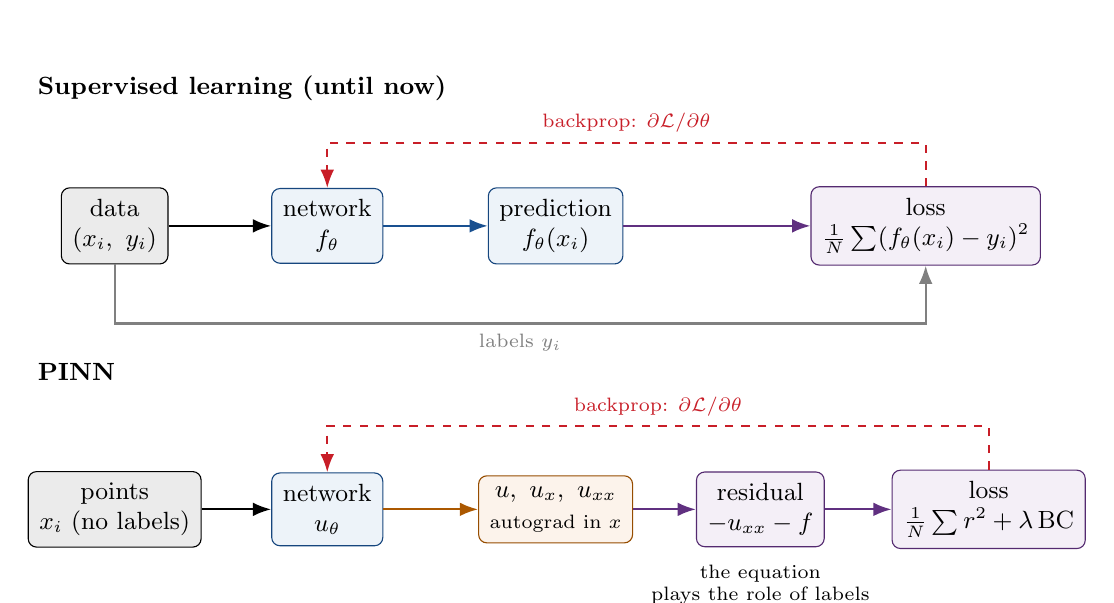
\begin{tikzpicture}[node distance=5mm]
% supervised learning
\node[font=\small\bfseries,anchor=west] at (-0.2,1.75) {Supervised learning (until now)};
\node[box=black] (d1) at (0.9,0) {data\\$(x_i,\ y_i)$};
\node[box=fwd]   (n1) at (3.6,0) {network\\$f_\theta$};
\node[box=fwd]   (p1) at (6.5,0) {prediction\\$f_\theta(x_i)$};
\node[box=lossc] (l1) at (11.2,0) {loss\\$\frac1N\sum(f_\theta(x_i)-y_i)^2$};
\draw[eg=black] (d1) -- (n1); \draw[eg=fwd] (n1) -- (p1); \draw[eg=lossc] (p1) -- (l1);
\draw[->,thick,black!50]   (d1.south) |- ++(0,-0.75) -| node[pos=0.25,below,font=\scriptsize] {labels $y_i$} (l1.south);
\draw[->,thick,dashed,bwd] (l1.north) -- ++(0,0.55)  -| node[pos=0.25,above,font=\scriptsize] {backprop: $\partial\loss/\partial\theta$} (n1.north);
% PINN
\begin{scope}[yshift=-3.6cm]
\node[font=\small\bfseries,anchor=west] at (-0.2,1.75) {PINN};
\node[box=black] (d2) at (0.9,0) {points\\$x_i$ (no labels)};
\node[box=fwd]   (n2) at (3.6,0) {network\\$u_\theta$};
\node[box=der]   (p2) at (6.5,0) {$u,\ u_x,\ u_{xx}$\\{\scriptsize autograd in $x$}};
\node[box=lossc] (r2) at (9.1,0) {residual\\$-u_{xx}-f$};
\node[box=lossc] (l2) at (12.0,0) {loss\\$\frac1N\sum r^2+\lambda\,\mathrm{BC}$};
\draw[eg=black] (d2) -- (n2); \draw[eg=der] (n2) -- (p2); \draw[eg=lossc] (p2) -- (r2); \draw[eg=lossc] (r2) -- (l2);
\node[font=\scriptsize,below=1mm of r2,align=center] {the equation\\plays the role of labels};
\draw[->,thick,dashed,bwd] (l2.north) -- ++(0,0.55) -| node[pos=0.25,above,font=\scriptsize] {backprop: $\partial\loss/\partial\theta$} (n2.north);
\end{scope}
\end{tikzpicture}

\small 지도학습과 PINN. 바뀐 것은 \textbf{loss를 만드는 방법}뿐이다. 정답 대신 방정식이 신경망을 평가한다.
학습 (역전파와 optimizer)은 지금까지와 똑같다.
\end{center}

\subsection{방정식이 주는 정보}

같은 신경망 (\ref{sec:poisson}절)을 세 가지 loss로 학습시킨다 (\texttt{data\_vs\_physics.py}).
\begin{enumerate}[label=(\Alph*),leftmargin=2em]
\item \textbf{데이터만}: $[0,0.4]$에서 측정한 $u^*$의 값 $8$개에 대한 최소제곱 (보통의 회귀).
\item \textbf{방정식만}: 식 \eqref{eq:pinnloss}.
\item \textbf{데이터 + 방정식}: 두 loss의 합.
\end{enumerate}

\begin{center}
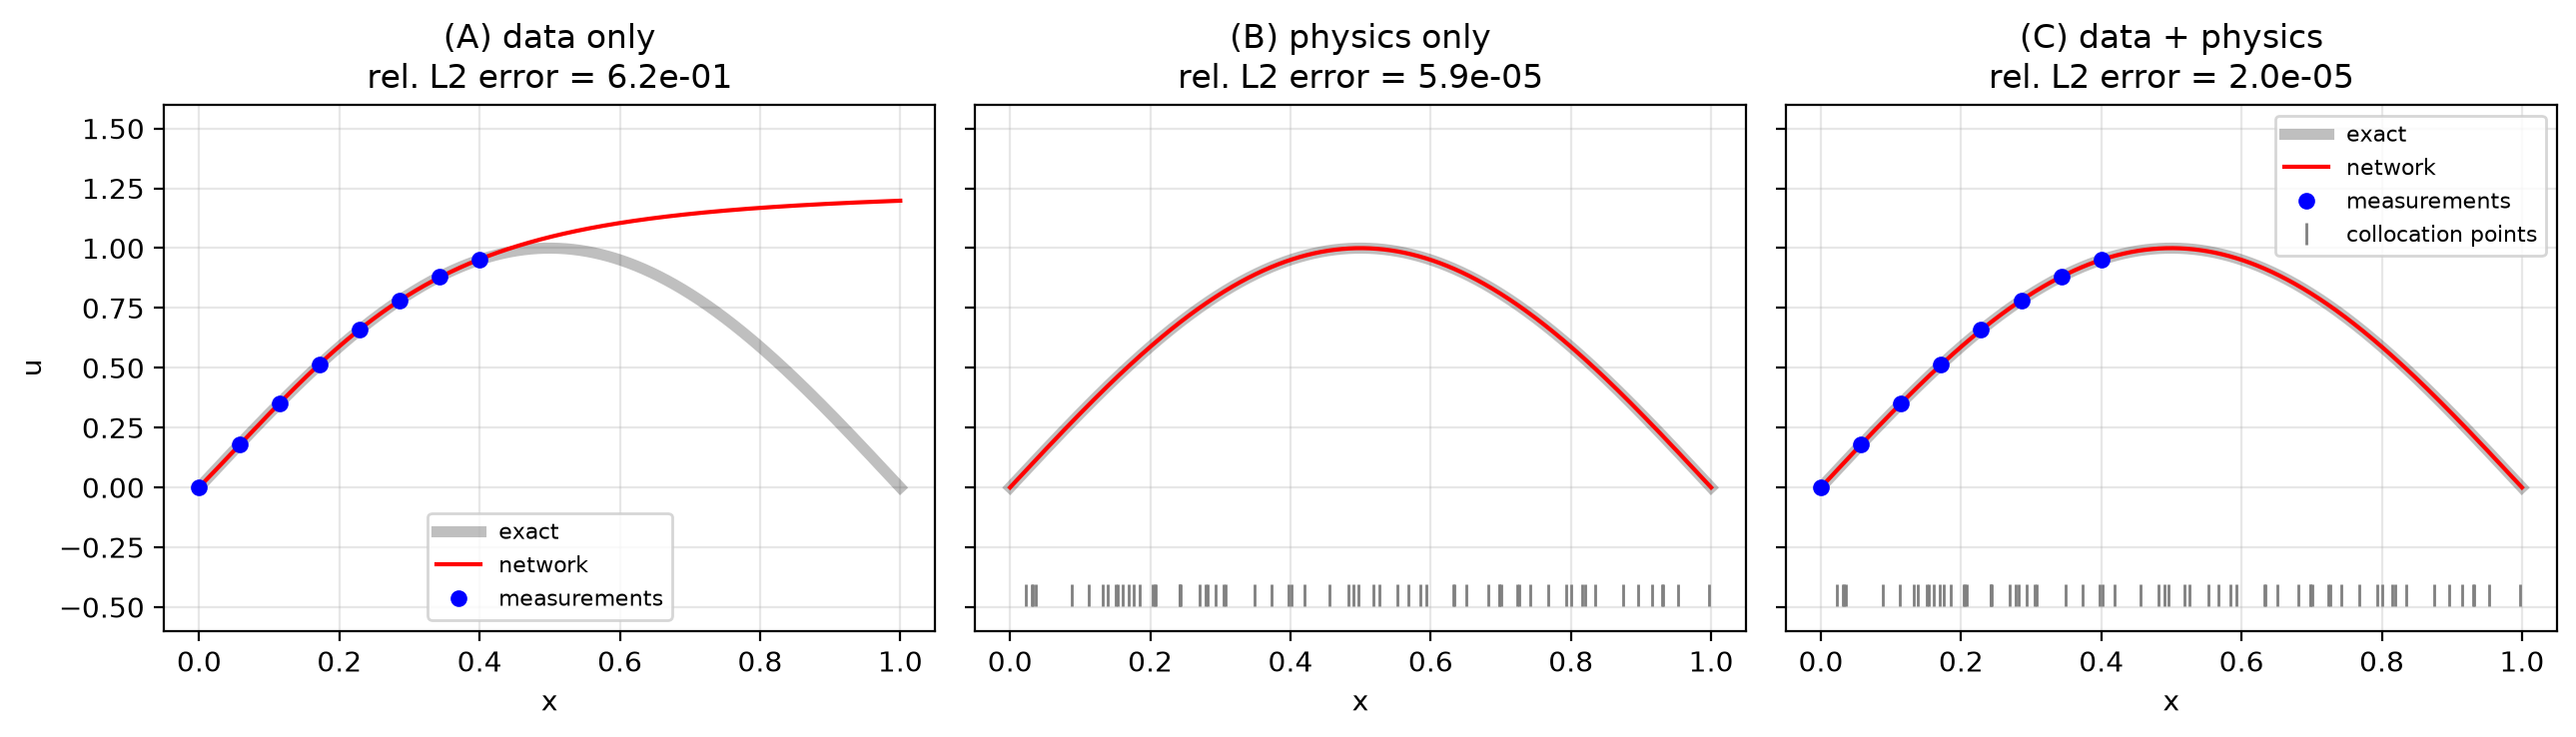
\includegraphics[width=\textwidth]{figures/data_vs_physics.png}

\small 측정값이 $[0,0.4]$에만 있을 때. (A)는 측정값이 없는 곳에서 엉뚱한 곡선을 그린다. (B)는 측정값 없이도 해를 찾는다.
\end{center}

해의 정확도는 \textbf{상대 $L^2$ 오차} (relative $L^2$ error)로 잰다. 시험점 $z_1,\dots,z_M$에서
\begin{equation}\label{eq:relerr}
\frac{\|u_\theta-u^*\|_2}{\|u^*\|_2}
=\left(\frac{\sum_{m=1}^M\big(u_\theta(z_m)-u^*(z_m)\big)^2}{\sum_{m=1}^M u^*(z_m)^2}\right)^{1/2}
\end{equation}
이고, 이는 $\int(u_\theta-u^*)^2$과 $\int(u^*)^2$을 점들의 합으로 근사한 비의 제곱근이다.
앞으로 해를 비교하는 상대오차는 모두 식 \eqref{eq:relerr}이다. 1차원 PINN의 시험점은 $[0,1]$의 등간격 $M=1001$개 점이다.

\begin{itemize}[leftmargin=1.5em]
\item (A) 상대오차 $0.62$. 측정값이 없는 $x>0.4$에서 해를 결정할 정보가 loss에 없다.
\item (B) 상대오차 $5.9\times10^{-5}$. 경계값 문제 \eqref{eq:poisson}의 해는 유일하므로, loss가 $0$인 함수는 $u^*$뿐이다.
\item (C) 상대오차 $2.0\times10^{-5}$. 방정식은 측정값이 없는 영역을, 측정값은 방정식에 없는 정보 (예: 미지의 계수, \ref{sec:inverse}절)를 준다.
\end{itemize}

\begin{remarkbox}[PINN의 역사]
신경망으로 미분방정식을 푸는 방법은 Lagaris, Likas, Fotiadis (1998)까지 거슬러 올라간다. 당시에는 $u_\theta''$의 식을 손으로 유도해 구현했다.
Raissi, Perdikaris, Karniadakis (2019)는 이 과정을 \textbf{자동미분}으로 일반화하고 ``Physics-Informed Neural Networks''라는 이름을 붙였다.
\end{remarkbox}

% =================================================
\section{신경망은 입력의 함수이다}\label{sec:smooth}
% =================================================

\subsection{두 종류의 미분}

신경망 $u_\theta(x)$는 입력 $x$와 매개변수 $\theta$의 함수이다.
학습에 쓰는 미분은 \textbf{매개변수에 대한 loss의 미분} $\partial\loss/\partial\theta$이고,
residual을 만드는 데 쓰는 미분은 \textbf{입력에 대한 출력의 미분} $\partial u_\theta/\partial x$이다.

\begin{center}
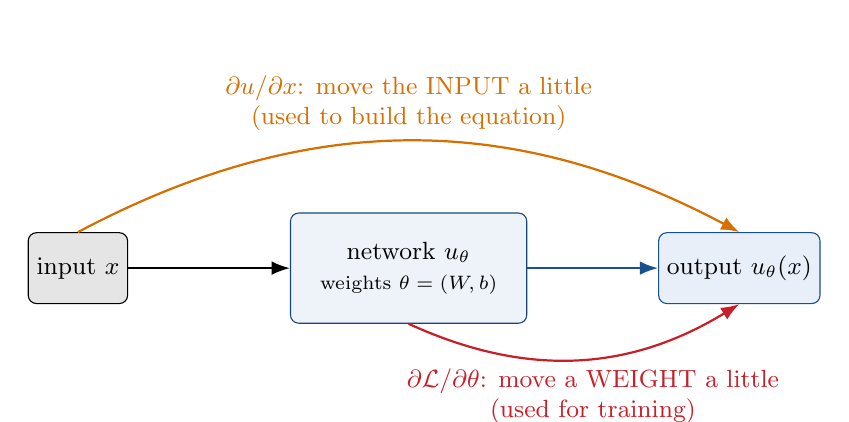
\begin{tikzpicture}
\node[box=fwd,minimum width=30mm,minimum height=14mm] (net) at (0,0) {network $u_\theta$\\{\scriptsize weights $\theta=(W,b)$}};
\node[val=black] (x) at (-4.2,0) {input $x$};
\node[val=fwd] (u) at (4.2,0) {output $u_\theta(x)$};
\draw[eg=black] (x) -- (net); \draw[eg=fwd] (net) -- (u);
\draw[->,thick,der,bend left=28] (x.north) to node[above,font=\small,align=center] {$\partial u/\partial x$: move the INPUT a little\\(used to build the equation)} (u.north);
\draw[->,thick,bwd,bend right=28] (net.south) to node[below,font=\small,align=center,pos=0.55] {$\partial \loss/\partial\theta$: move a WEIGHT a little\\(used for training)} (u.south);
\end{tikzpicture}
\end{center}

\begin{center}
\begin{tabular}{@{}lll@{}}
\toprule
& $\partial\loss/\partial\theta$ & $\partial u_\theta/\partial x$ \\
\midrule
무엇을 움직이는가 & 가중치 $\theta$ & 입력 $x$ (가중치는 고정) \\
어디에 쓰는가 & 경사하강법으로 학습 & 방정식 (residual)을 만들 때 \\
PyTorch & \texttt{loss.backward()} & \texttt{torch.autograd.grad(u, x, ...)} \\
결과의 모양 & 가중치와 같은 모양 & 입력과 같은 모양 $(N,1)$ \\
\bottomrule
\end{tabular}
\end{center}

두 미분 모두 계산 그래프 위의 연쇄법칙이다. 자동미분에게 입력 $x$는 가중치와 같은 \textbf{잎(leaf) 노드}이고, 미분하는 잎 노드가 다를 뿐이다.

\subsection{활성화 함수는 매끄러워야 한다: tanh와 ReLU}

식 \eqref{eq:poisson}의 residual에는 $u_\theta''$가 들어가므로 $u_\theta$는 두 번 미분 가능해야 한다.
은닉층이 하나이면
\[
u_\theta(x)=\sum_{j} v_j\,\sigma(w_jx+b_j)+c
\quad\Longrightarrow\quad
u_\theta''(x)=\sum_j v_j\,w_j^2\,\sigma''(w_jx+b_j).
\]
즉 $u_\theta''$는 $\sigma''$의 선형결합이다.

\begin{itemize}[leftmargin=1.5em]
\item $\tanh\in C^\infty$: $\tanh'(a)=1-\tanh^2(a)$, $\ \tanh''(a)=-2\tanh(a)\big(1-\tanh^2(a)\big)$.
\item ReLU는 구간별 일차함수이다. $a\ne0$에서 $\mathrm{ReLU}''(a)=0$이므로 ReLU 신경망은 \textbf{거의 모든 $x$에서 $u_\theta''=0$}이다.
\end{itemize}

\begin{center}
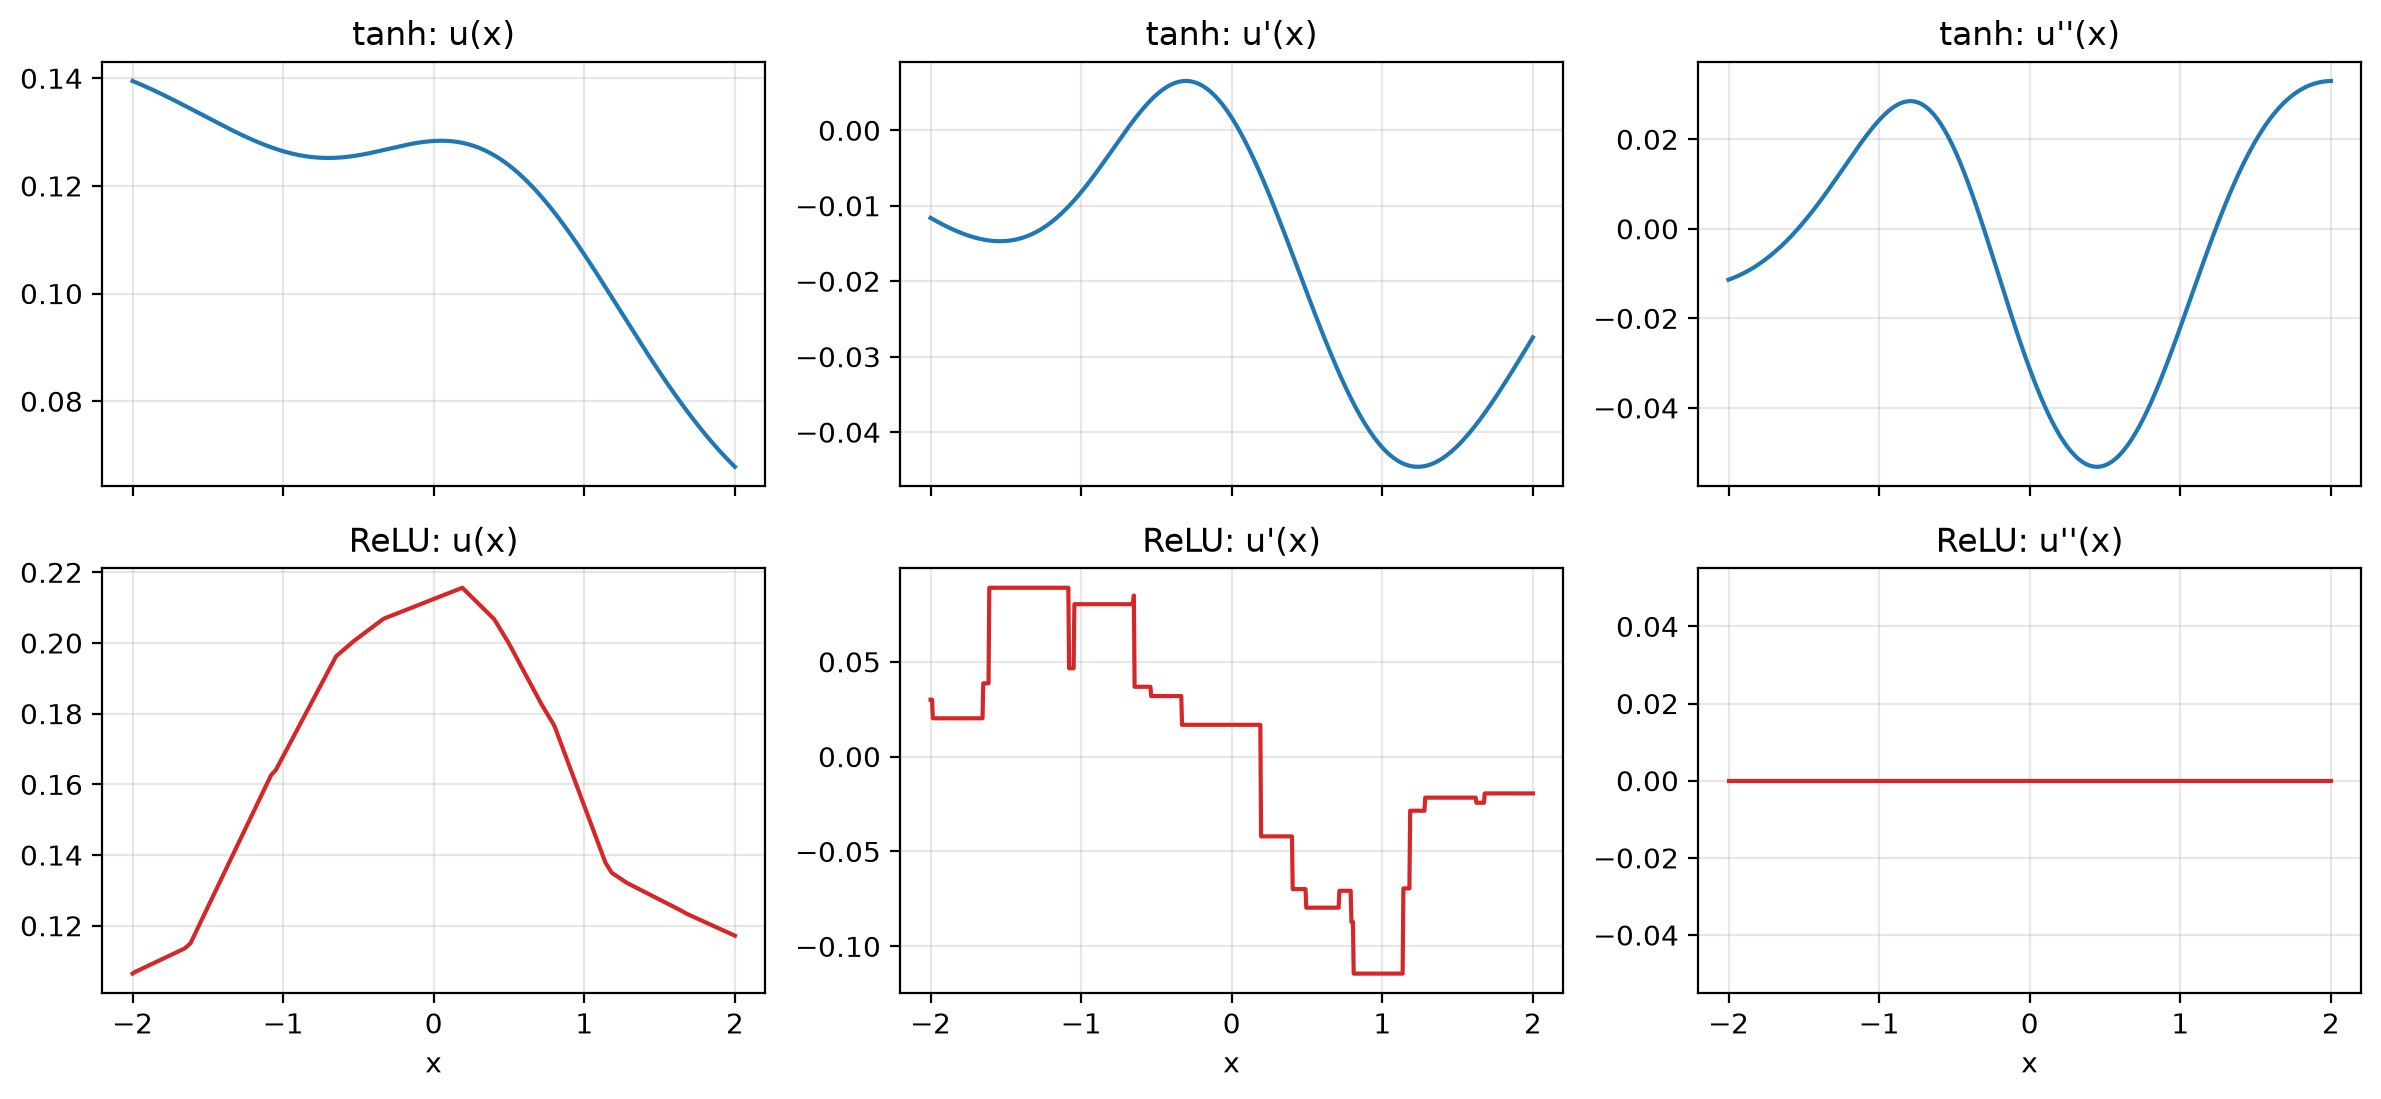
\includegraphics[width=\textwidth]{figures/tanh_vs_relu.png}

\small 무작위 가중치를 가진 두 신경망 ($1\to16\to16\to1$)과 그 도함수 (\texttt{tanh\_vs\_relu.py}). 모두 autograd로 계산하였다.
ReLU 신경망은 꺾은선이고, $u'$는 계단, $u''$는 정확히 $0$이다.
\end{center}

\begin{thinkbox}[ReLU로 PINN을 만들면 오류가 나는가?]
나지 않는다. autograd는 ReLU의 2계 도함수를 $0$으로 계산한다
(\texttt{tanh\_vs\_relu.py}의 출력: \texttt{ReLU: max |u\_xx| on [-2, 2] = 0.000e+00}).
그러면 $r=-f$가 $\theta$와 무관해져 PDE 항의 gradient가 $0$이 되고, 학습은 오류 없이 실패한다.
PINN에는 $\tanh$, $\sin$, softplus, SiLU처럼 매끄러운 활성화 함수를 쓴다.
\end{thinkbox}

% =================================================
\section{계산 그래프로 끝까지 따라가기}\label{sec:graph}
% =================================================

PINN 학습 한 step의 계산을 은닉 뉴런 하나짜리 신경망에서 노드 단위로 따라간다.
숫자는 \texttt{autograd\_tiny.py}의 출력이며, 손계산과 소수점 다섯째 자리까지 일치한다.

\subsection{가장 작은 신경망과 그 계산 그래프}\label{sec:tiny}

입력 $1$개, 은닉 뉴런 $1$개, 출력 $1$개인 신경망
\[
u(x)=w_2\tanh(w_1x+b_1)+b_2
\]
을 생각하자. 가중치는 $w_1=0.8$, $b_1=-0.2$, $w_2=1.5$, $b_2=0.3$이고, 입력은 $x=1$이다.
중간값에 이름을 붙이면
\[
a=w_1x+b_1=0.6,\qquad h=\tanh(a)=0.53705,\qquad u=w_2h+b_2=1.10557.
\]

\begin{center}
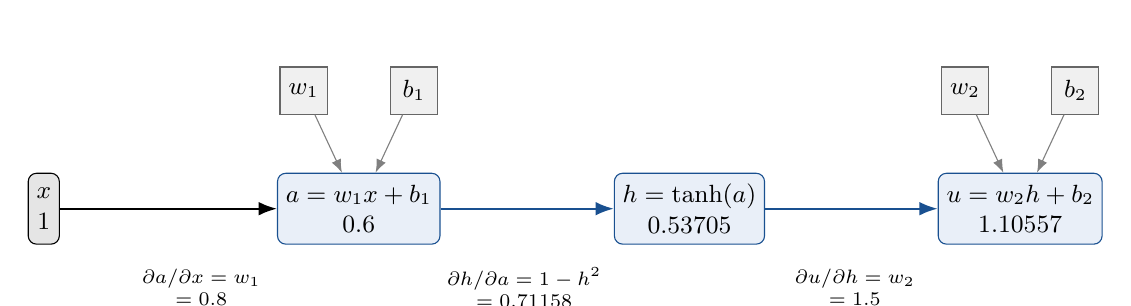
\begin{tikzpicture}
\node[val=black] (x) at (0,0) {$x$\\$1$};
\node[val=fwd] (a) at (4.0,0) {$a=w_1x+b_1$\\$0.6$};
\node[val=fwd] (h) at (8.2,0) {$h=\tanh(a)$\\$0.53705$};
\node[val=fwd] (u) at (12.4,0) {$u=w_2h+b_2$\\$1.10557$};
\node[par] (w1) at (3.3,1.5) {$w_1$}; \node[par] (b1) at (4.7,1.5) {$b_1$};
\node[par] (w2) at (11.7,1.5) {$w_2$}; \node[par] (b2) at (13.1,1.5) {$b_2$};
\draw[eg=black] (x) -- (a);
\draw[eg=fwd] (a) -- (h);
\draw[eg=fwd] (h) -- (u);
\node[font=\scriptsize,align=center] at (2.0,-1.0) {$\partial a/\partial x=w_1$\\$=0.8$};
\node[font=\scriptsize,align=center] at (6.1,-1.0) {$\partial h/\partial a=1-h^2$\\$=0.71158$};
\node[font=\scriptsize,align=center] at (10.3,-1.0) {$\partial u/\partial h=w_2$\\$=1.5$};
\foreach \p/\q in {w1/a,b1/a,w2/u,b2/u} \draw[->,black!50] (\p) -- (\q);
\end{tikzpicture}

\small 원래 계산 그래프 (forward). 둥근 상자는 중간값, 네모는 가중치 (잎 노드)이다.
화살표 아래에는 그 화살표의 \textbf{국소 미분} (앞 노드가 조금 변할 때 뒤 노드가 변하는 비율)을 적었다.
\end{center}

\subsection{입력에 대한 미분: 미분 그래프가 새로 생긴다}\label{sec:ux}

연쇄법칙에 따라 $u_x=\partial u/\partial x$는 $x$에서 $u$까지 가는 경로 위의 국소 미분을 모두 곱한 것이다.
\[
u_x=\pd{u}{h}\,\pd{h}{a}\,\pd{a}{x}=w_2\cdot(1-h^2)\cdot w_1=1.5\times0.71158\times0.8=0.85389.
\]
여기서 $s=1-h^2$로 둔다.

\begin{keybox}[관찰 1: $u_x$는 숫자가 아니라 새로운 계산이다]
$u_x=w_2\,s\,w_1$, $s=1-h^2$. $u_x$를 계산하려면 원래 그래프의 노드 $h$와 가중치 $w_1,w_2$로부터 새 연산을 해야 한다.
이 연산들이 \textbf{미분 그래프}를 이루며, 미분 그래프는 원래 그래프의 노드를 입력으로 \textbf{공유}한다.
\end{keybox}

\begin{center}
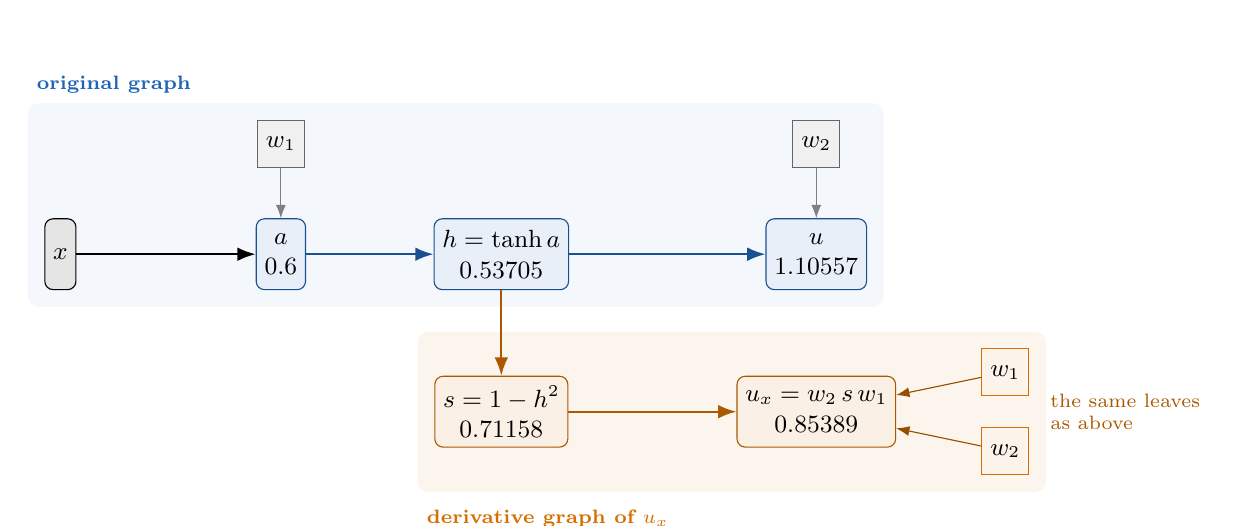
\begin{tikzpicture}
% forward row
\node[val=black] (x) at (0,0) {$x$};
\node[val=fwd] (a) at (2.8,0) {$a$\\$0.6$};
\node[val=fwd] (h) at (5.6,0) {$h=\tanh a$\\$0.53705$};
\node[val=fwd] (u) at (9.6,0) {$u$\\$1.10557$};
\node[par] (w1) at (2.8,1.4) {$w_1$};
\node[par] (w2) at (9.6,1.4) {$w_2$};
\draw[eg=black] (x) -- (a); \draw[eg=fwd] (a) -- (h); \draw[eg=fwd] (h) -- (u);
\draw[->,black!50] (w1) -- (a); \draw[->,black!50] (w2) -- (u);
% derivative row
\node[val=der] (s) at (5.6,-2.0) {$s=1-h^2$\\$0.71158$};
\node[val=der] (ux) at (9.6,-2.0) {$u_x=w_2\,s\,w_1$\\$0.85389$};
\draw[eg=der] (h) -- (s);
\draw[eg=der] (s) -- (ux);
\node[par,draw=der,fill=der!8] (w1c) at (12.0,-1.5) {$w_1$};
\node[par,draw=der,fill=der!8] (w2c) at (12.0,-2.5) {$w_2$};
\draw[->,der!70!black] (w1c) -- (ux); \draw[->,der!70!black] (w2c) -- (ux);
\node[font=\scriptsize,der!80!black,align=left,anchor=west] at (12.45,-2.0) {the same leaves\\as above};
\begin{scope}[on background layer]
\node[fill=fwd!5,rounded corners,fit=(x)(a)(h)(u)(w1)(w2),inner sep=6pt] (F) {};
\node[fill=der!7,rounded corners,fit=(s)(ux)(w1c)(w2c),inner sep=6pt] (D) {};
\end{scope}
\node[font=\scriptsize\bfseries,fwd,anchor=south west] at (F.north west) {original graph};
\node[font=\scriptsize\bfseries,der,anchor=north west] at ([yshift=-1mm]D.south west) {derivative graph of $u_x$};
\end{tikzpicture}

\small 파란색은 원래 그래프, 주황색은 $u_x$를 계산하는 미분 그래프이다.
미분 그래프는 원래 그래프의 노드 $h$와 가중치 $w_1$, $w_2$를 재료로 쓴다.
\end{center}

PyTorch의 그래프로 확인하자. \texttt{autograd\_tiny.py}의 5번 셀은 \texttt{grad\_fn}을 따라가며 그래프를 출력한다
(들여쓰기가 깊을수록 입력 쪽, 이름의 뜻은 \ref{sec:nodes}절). $u$의 그래프:
\begin{lstlisting}[language={},numbers=none]
AddBackward0                          u = (w2 * h) + b2
  MulBackward0                        w2 * h
    AccumulateGrad  (leaf: w2)
    TanhBackward0                     h = tanh(a)
      AddBackward0                    a = (w1 * x) + b1
        MulBackward0                  w1 * x
          AccumulateGrad  (leaf: w1)
          AccumulateGrad  (leaf: x)
        AccumulateGrad  (leaf: b1)
  AccumulateGrad  (leaf: b2)
\end{lstlisting}
\texttt{torch.autograd.grad(u, x, create\_graph=True)}로 얻은 $u_x$의 그래프:
\begin{lstlisting}[language={},numbers=none]
MulBackward0                          u_x = [tanh'(a) * w2] * w1
  TanhBackwardBackward0               tanh'(a) * w2 = (1 - h^2) * w2   <- a NEW node
    MulBackward0                      (the incoming gradient du/du * w2 = w2)
      AccumulateGrad  (leaf: w2)
    TanhBackward0                     <- the node h of the ORIGINAL graph, reused
      AddBackward0
        MulBackward0
          AccumulateGrad  (leaf: w1)
          AccumulateGrad  (leaf: x)
        AccumulateGrad  (leaf: b1)
  AccumulateGrad  (leaf: w1)
\end{lstlisting}
오른쪽 주석은 우리가 붙인 것이다. \texttt{TanhBackwardBackward0}은 tanh의 역전파 연산 $(1-h^2)\times w_2$를 미분 가능한 노드로 기록한 것이고,
그 아래에서 원래 그래프의 \texttt{TanhBackward0} ($h$)가 재사용된다. 위 그림의 주황색 부분이다.

\subsection{한 번 더 미분하기: $u_{xx}$}\label{sec:uxx}

$u_x=w_2\,w_1\,s$를 $x$로 한 번 더 미분하자. $w_1,w_2$는 $x$와 무관하고, $s=1-h^2$는 $a$를 통해 $x$에 의존한다.
\[
\pd{s}{a}=-2h\,\pd{h}{a}=-2hs,\qquad
u_{xx}=w_2\,w_1\,\pd{s}{a}\,\pd{a}{x}=w_2\,w_1^2\,(-2hs).
\]
숫자를 넣으면 $-2hs=-0.76431$, $u_{xx}=1.5\times0.64\times(-0.76431)=-0.73373$이다.
미분 그래프가 한 층 더 자란다. \texttt{autograd\_tiny.py}가 센 그래프의 노드 수 (잎 노드 포함)는 다음과 같다.
\begin{center}
\begin{tabular}{@{}lcccc@{}}
\toprule
텐서 & $u$ & $u_x$ & $u_{xx}$ & $\loss$ \\
\midrule
그래프의 노드 수 & $10$ & $10$ & $14$ & $19$ \\
\bottomrule
\end{tabular}
\end{center}
$u_x$의 그래프는 $u$의 그래프를 공유하며 노드를 더하고, $u_{xx}$는 다시 그 위에 노드를 더한다.
미분할 때마다 그래프가 커지므로, PINN 한 step의 계산량과 메모리는 같은 신경망의 보통 학습보다 크다.

\subsection{원래 그래프와 미분 그래프가 만나는 곳: residual과 loss}\label{sec:loss}

원래 그래프와 미분 그래프가 모두 residual에 들어가도록 상미분방정식 $u''+u=0$을 예로 든다.
점 $x=1$에서
\[
r=u_{xx}+u=-0.73373+1.10557=0.37184,\qquad \loss=r^2=0.13827.
\]
$r$에서 원래 그래프의 출력 $u$와 미분 그래프의 출력 $u_{xx}$가 \textbf{만난다}. 전체 그래프는 다음과 같다.

\begin{center}
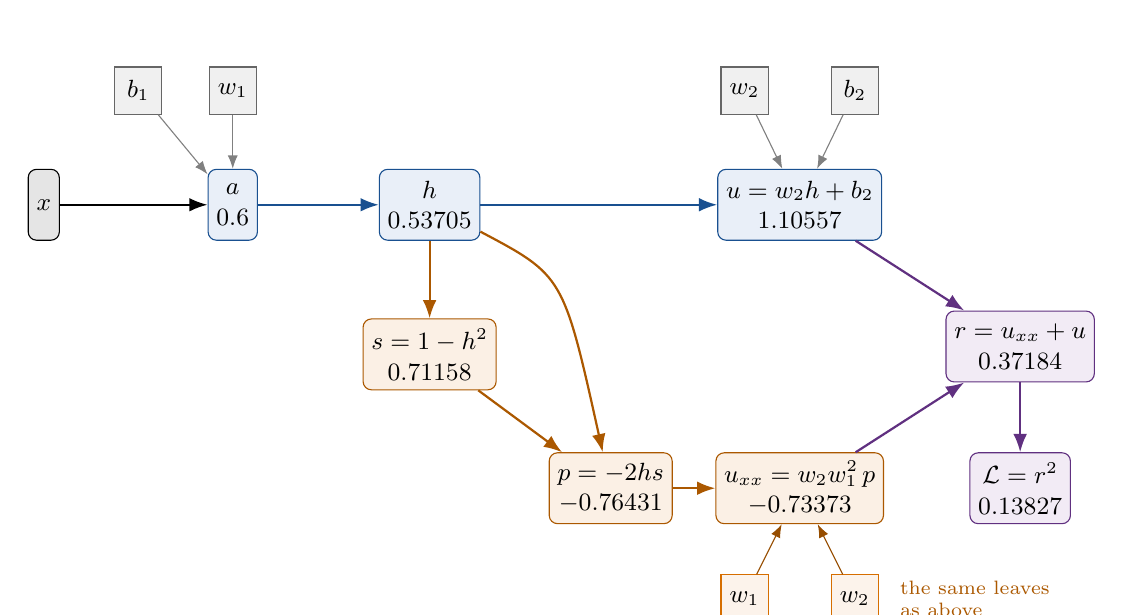
\begin{tikzpicture}
% forward row
\node[val=black] (x) at (0,0) {$x$};
\node[val=fwd] (a) at (2.4,0) {$a$\\$0.6$};
\node[val=fwd] (h) at (4.9,0) {$h$\\$0.53705$};
\node[val=fwd] (u) at (9.6,0) {$u=w_2h+b_2$\\$1.10557$};
\node[par] (w1) at (2.4,1.45) {$w_1$}; \node[par] (b1) at (1.2,1.45) {$b_1$};
\node[par] (w2) at (8.9,1.45) {$w_2$}; \node[par] (b2) at (10.3,1.45) {$b_2$};
\draw[eg=black] (x) -- (a); \draw[eg=fwd] (a) -- (h); \draw[eg=fwd] (h) -- (u);
\draw[->,black!50] (w1) -- (a); \draw[->,black!50] (b1) -- (a);
\draw[->,black!50] (w2) -- (u); \draw[->,black!50] (b2) -- (u);
% derivative rows
\node[val=der] (s) at (4.9,-1.9) {$s=1-h^2$\\$0.71158$};
\node[val=der] (p) at (7.2,-3.6) {$p=-2hs$\\$-0.76431$};
\node[val=der] (uxx) at (9.6,-3.6) {$u_{xx}=w_2w_1^2\,p$\\$-0.73373$};
\draw[eg=der] (h) -- (s);
\draw[eg=der] (s) -- (p);
\draw[eg=der] (h) .. controls (6.6,-0.9) .. (p);
\draw[eg=der] (p) -- (uxx);
\node[par,draw=der,fill=der!8] (w1c) at (8.9,-5.0) {$w_1$}; \node[par,draw=der,fill=der!8] (w2c) at (10.3,-5.0) {$w_2$};
\draw[->,der!70!black] (w1c) -- (uxx); \draw[->,der!70!black] (w2c) -- (uxx);
\node[font=\scriptsize,der!80!black,align=left,anchor=west] at (10.75,-5.0) {the same leaves\\as above};
% residual and loss
\node[val=lossc] (r) at (12.4,-1.8) {$r=u_{xx}+u$\\$0.37184$};
\node[val=lossc] (L) at (12.4,-3.6) {$\loss=r^2$\\$0.13827$};
\draw[eg=lossc] (u) -- (r); \draw[eg=lossc] (uxx) -- (r); \draw[eg=lossc] (r) -- (L);
\end{tikzpicture}

\small 학습 한 step의 전체 그래프. 파란색: 원래 그래프, 주황색: 미분 그래프 ($u_x$의 노드는 $u_{xx}$로 정리하여 생략),
보라색: residual과 loss. $w_1$, $w_2$는 원래 그래프와 미분 그래프 \textbf{양쪽에} 들어간다.
\end{center}

\begin{keybox}[관찰 2: loss는 하나의 큰 그래프의 출력이다]
residual $r$에서 원래 그래프와 미분 그래프는 \textbf{하나의 그래프}가 된다.
PyTorch에게 미분 그래프는 특별한 것이 아니다. 덧셈, 곱셈, tanh 노드로 이루어진 그래프이고 그 끝에 스칼라 $\loss$가 있다.
따라서 \texttt{loss.backward()}는 보통의 역전파와 같다.
\end{keybox}

\subsection{역전파: gradient는 여러 경로를 거쳐 더해진다}\label{sec:backward}

\texttt{loss.backward()}는 $\loss$에서 그래프를 거꾸로 따라가며 $\partial\loss/\partial\theta$를 구한다.
한 가중치가 그래프의 여러 곳에 나타나면, 다변수 연쇄법칙에 따라 \textbf{경로별 기여를 더한다}.

$\loss=r^2$이므로 $\partial\loss/\partial\theta=2r\cdot\partial r/\partial\theta$이고, $2r=0.74368$이다.
$r=u_{xx}+u=w_2w_1^2\,p+w_2h+b_2$를 각 가중치로 미분하자.

\paragraph{$b_2$:} $b_2$는 $u$에만 있다. 경로가 하나이므로 $\partial r/\partial b_2=1$.

\paragraph{$w_2$:} $w_2$는 $u$와 $u_{xx}$ 두 곳에 있다.
\[
\pd{r}{w_2}=\underbrace{h}_{\text{via }u}+\underbrace{w_1^2\,p}_{\text{via }u_{xx}}=0.53705+(-0.48916)=0.04789.
\]

\paragraph{$w_1$:} $w_1$에서 $r$로 가는 경로는 \textbf{세 개}이다.
\begin{center}
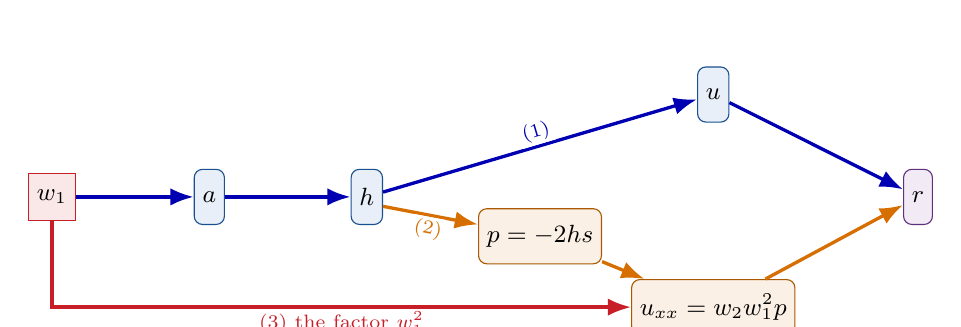
\begin{tikzpicture}[val/.style={draw=#1!80!black,fill=#1!10,rounded corners=3pt,align=center,font=\small,inner sep=3pt,minimum height=7mm}]
\node[par,fill=bwd!10,draw=bwd] (w1) at (0,0) {$w_1$};
\node[val=fwd] (a) at (2.0,0) {$a$};
\node[val=fwd] (h) at (4.0,0) {$h$};
\node[val=fwd] (u) at (8.4,1.3) {$u$};
\node[val=der] (p) at (6.2,-0.5) {$p=-2hs$};
\node[val=der] (uxx) at (8.4,-1.4) {$u_{xx}=w_2w_1^2p$};
\node[val=lossc] (r) at (11.0,0) {$r$};
\draw[->,very thick,blue!70!black] (w1) -- (a);
\draw[->,very thick,blue!70!black] (a) -- (h);
\draw[->,very thick,blue!70!black] (h) -- node[elab,above,sloped] {(1)} (u);
\draw[->,very thick,blue!70!black] (u) -- (r);
\draw[->,very thick,der] ([yshift=-1.2mm]h.east) -- node[elab,below,sloped] {(2)} (p);
\draw[->,very thick,der] (p) -- (uxx);
\draw[->,very thick,der] (uxx) -- (r);
\draw[->,very thick,bwd] (w1.south) |- node[elab,pos=0.75,below] {(3) the factor $w_1^2$} (uxx.west);
\end{tikzpicture}
\end{center}
\begin{align*}
\pd{r}{w_1}
&=\underbrace{w_2\,s\,x}_{(1)\ w_1\to a\to h\to u}
+\underbrace{w_2\,w_1^2\,\pd{p}{a}\,x}_{(2)\ w_1\to a\to h\to p\to u_{xx}}
+\underbrace{w_2\cdot2w_1\cdot p}_{(3)\ w_1\to u_{xx}}\\
&=1.06737+(-0.18408)+(-1.83433)=-0.95104.
\end{align*}
여기서 $\partial p/\partial a=\partial(-2hs)/\partial a=-2s(1-3h^2)=-0.19175$이다.
경로 (1)은 보통의 역전파 경로이고, (2), (3)은 미분 그래프를 지나는 경로이다.
이 예에서는 (2)+(3)의 기여 $-2.02$가 (1)의 $1.07$보다 크고 부호가 반대이다.

\paragraph{$b_1$:} $b_1$은 $a$에만 있지만, $a$에서 $r$로 가는 경로가 (1)과 (2) 두 개이다.
$\partial r/\partial b_1=w_2s+w_2w_1^2\,\partial p/\partial a=1.06737-0.18408=0.88329$.

\begin{center}
\begin{tabular}{@{}lcccc@{}}
\toprule
& $w_1$ & $b_1$ & $w_2$ & $b_2$ \\
\midrule
손계산 $2r\cdot\partial r/\partial\theta$ & $-0.70727$ & $0.65689$ & $0.03562$ & $0.74368$ \\
autograd (\texttt{.grad}) & $-0.70727$ & $0.65689$ & $0.03562$ & $0.74368$ \\
\bottomrule
\end{tabular}
\end{center}

\begin{thinkbox}[활성화 함수는 몇 번 미분 가능해야 하는가]
경로 (2)의 $\partial p/\partial a$는 $\tanh$의 \textbf{3계 도함수}이다. loss의 $u_{xx}$를 다시 가중치로 미분하기 때문이다.
일반적으로 residual에 $k$계 도함수가 있으면 역전파에는 활성화 함수의 $(k+1)$계 도함수가 필요하다.
PyTorch는 이것도 그래프로 처리한다 (\texttt{TanhBackwardBackward0}을 미분하는 노드가 생긴다).
\end{thinkbox}

\subsection{학습 한 step에서 일어나는 일}\label{sec:onestep}

학습 한 step을 정리하면 다음과 같다.
\begin{center}
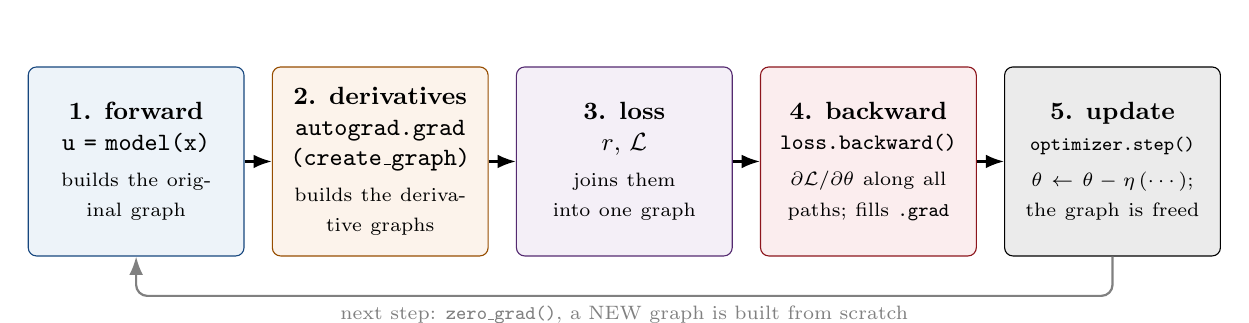
\begin{tikzpicture}[st/.style={draw=#1!70!black,fill=#1!8,rounded corners=3pt,align=center,font=\small,text width=26mm,minimum height=24mm,inner sep=2pt}]
\node[st=fwd] (s1) at (0,0) {\textbf{1. forward}\\\texttt{u = model(x)}\\[2pt]{\scriptsize builds the original graph}};
\node[st=der] (s2) at (3.1,0) {\textbf{2. derivatives}\\\texttt{autograd.grad}\\\texttt{(create\_graph)}\\[2pt]{\scriptsize builds the derivative graphs}};
\node[st=lossc] (s3) at (6.2,0) {\textbf{3. loss}\\$r$, $\loss$\\[2pt]{\scriptsize joins them into one graph}};
\node[st=bwd] (s4) at (9.3,0) {\textbf{4. backward}\\{\footnotesize\texttt{loss.backward()}}\\[2pt]{\scriptsize $\partial\loss/\partial\theta$ along all paths; fills \texttt{.grad}}};
\node[st=black] (s5) at (12.4,0) {\textbf{5. update}\\{\scriptsize\texttt{optimizer.step()}}\\[2pt]{\scriptsize $\theta\leftarrow\theta-\eta\,(\cdots)$; the graph is freed}};
\foreach \i/\j in {s1/s2,s2/s3,s3/s4,s4/s5} \draw[->,thick] (\i) -- (\j);
\draw[->,thick,black!50,rounded corners] (s5.south) -- ++(0,-0.5) -| node[pos=0.25,below,font=\scriptsize] {next step: \texttt{zero\_grad()}, a NEW graph is built from scratch} (s1.south);
\end{tikzpicture}
\end{center}
\begin{itemize}[leftmargin=1.5em]
\item 1--3단계에서 그래프가 만들어진다. 2단계의 미분은 값을 계산하면서 그 계산을 그래프에 기록한다.
\item 4단계는 그래프를 거꾸로 한 번 지나간다. 보통의 역전파와 다른 것은 그래프의 크기뿐이다.
\item 5단계의 optimizer는 \texttt{.grad}만 사용하며, 2단계와 무관하다.
\item 그래프는 step마다 새로 만들어지고 \texttt{backward()} 후에 해제된다.
\end{itemize}

\begin{keybox}[PINN 학습 한 step의 세 가지 미분]
\begin{enumerate}[leftmargin=1.5em]
\item \texttt{torch.autograd.grad(u, x, create\_graph=True)}: \textbf{입력}에 대한 미분 $u_x$, $u_{xx}$. 결과를 돌려주고, 계산 과정을 그래프에 \textbf{추가}한다.
\item \texttt{loss.backward()}: \textbf{가중치}에 대한 미분 $\partial\loss/\partial\theta$. 원래 그래프와 미분 그래프의 모든 경로를 거쳐 더한 값을 각 가중치의 \texttt{.grad}에 넣는다.
\item \texttt{optimizer.step()}: 미분이 아니라 \textbf{갱신}. \texttt{.grad}를 이용해 가중치를 바꾼다.
\end{enumerate}
\end{keybox}

% =================================================
\section{PyTorch에서 입력으로 미분하기}\label{sec:torch}
% =================================================

코드를 읽는 데 필요한 세부 사항이다. \texttt{autograd\_tiny.py}를 셀 단위로 실행하며 읽자.

\subsection{그래프의 노드는 연산이다}\label{sec:nodes}

\ref{sec:ux}절의 출력에 나온 \texttt{AddBackward0}, \texttt{grad\_fn} 같은 이름의 뜻을 정리한다.
이 절의 출력은 모두 \texttt{autograd\_tiny.py}의 8번 셀에서 나온 것이다.

\ref{sec:graph}절의 그림에서는 값 $h$, $u$를 노드로 그렸다. PyTorch가 저장하는 노드는 \textbf{연산}이고, 텐서는 노드 사이를 흐른다.
중간값 하나를 만드는 연산은 정확히 하나이므로 두 표기는 일대일로 대응한다. 그림의 노드 $h$는 PyTorch의 \texttt{TanhBackward0}이다.

forward 계산은 실행되고 지나갈 뿐, forward 그래프가 따로 저장되지는 않는다.
PyTorch는 연산을 실행할 때마다 그 연산을 거꾸로 미분하는 \textbf{역방향 노드}를 하나 만들어, 입력 쪽의 노드에 연결한다.
\begin{lstlisting}
m = w1 * x          # m.grad_fn = MulBackward0
a = m + b1          # a.grad_fn = AddBackward0
h = torch.tanh(a)   # h.grad_fn = TanhBackward0
p = w2 * h          # p.grad_fn = MulBackward0
u = p + b2          # u.grad_fn = AddBackward0
\end{lstlisting}
\texttt{grad\_fn}은 gradient function의 줄임말이다. 텐서의 속성이고, 그 텐서를 만든 연산의 역방향 노드를 가리킨다.
\texttt{AddBackward0}, \texttt{MulBackward0}, \texttt{TanhBackward0}은 덧셈, 곱셈, $\tanh$의 역방향 노드의 이름이다.
\texttt{AccumulateGrad}는 잎 텐서 전용의 종착 노드로, 도착한 값을 그 텐서의 \texttt{.grad}에 더한다.

\begin{center}
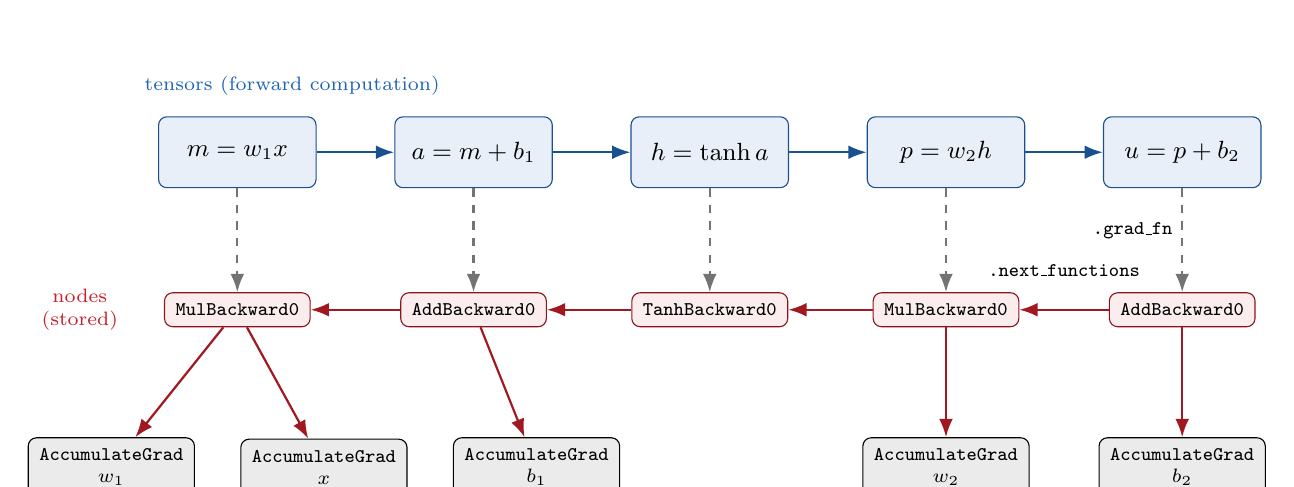
\begin{tikzpicture}
\foreach \n/\xx/\lab in {m/1/{$m=w_1x$}, a/4/{$a=m+b_1$}, h/7/{$h=\tanh a$}, p/10/{$p=w_2h$}, u/13/{$u=p+b_2$}}
  \node[val=fwd,minimum width=20mm] (t\n) at (\xx,0) {\lab};
\foreach \n/\xx/\lab in {m/1/MulBackward0, a/4/AddBackward0, h/7/TanhBackward0, p/10/MulBackward0, u/13/AddBackward0}
  \node[box=bwd,font=\scriptsize\ttfamily] (n\n) at (\xx,-2) {\lab};
\foreach \n/\xx/\lab in {wa/-0.6/$w_1$, x/2.1/$x$, b/4.8/$b_1$, wb/10/$w_2$, bb/13/$b_2$}
  \node[box=black,font=\scriptsize] (l\n) at (\xx,-4) {\texttt{AccumulateGrad}\\\lab};
\foreach \i/\j in {m/a,a/h,h/p,p/u} \draw[eg=fwd] (t\i) -- (t\j);
\foreach \n in {m,a,h,p,u} \draw[->,thick,dashed,black!55] (t\n) -- (n\n);
\foreach \i/\j in {u/p,p/h,h/a,a/m} \draw[eg=bwd] (n\i) -- (n\j);
\foreach \i/\j in {m/wa,m/x,a/b,p/wb,u/bb} \draw[eg=bwd] (n\i) -- (l\j);
\node[font=\scriptsize\ttfamily,left] at (13,-1.0) {.grad\_fn};
\node[font=\scriptsize\ttfamily] at (11.5,-1.5) {.next\_functions};
\node[font=\scriptsize,fwd,anchor=west] at (-0.3,0.85) {tensors (forward computation)};
\node[font=\scriptsize,bwd,align=center] at (-1,-2) {nodes\\(stored)};
\end{tikzpicture}

\small 위: 계산되는 텐서. 가운데와 아래: 저장되는 역방향 그래프. 텐서는 \texttt{grad\_fn}으로 자기를 만든 노드 하나만 가리키고, 그 뒤의 연결은 노드들끼리 \texttt{next\_functions}로 이어진다.
\end{center}

그래프는 코드가 실행되는 그 순간에 만들어지므로 (define-by-run), \texttt{if}나 \texttt{for}로 실행한 연산이 곧 그래프의 모양이다.
\texttt{nn.Module} 객체는 그래프가 아니다. 가중치와 \texttt{forward} 코드만 갖고 있고, 그래프는 \texttt{model(x)}를 실행할 때 생긴다.

\subsection{텐서의 속성과 메서드}

텐서는 \texttt{torch.Tensor} 클래스의 객체이고, 값 외에 다음을 갖는다. 괄호 없이 읽으면 \textbf{속성} (attribute), 괄호를 붙여 호출하면 \textbf{메서드} (method)이다.
\begin{center}
\begin{tabular}{@{}lp{112mm}@{}}
\toprule
속성 & 내용 \\
\midrule
\texttt{.grad} & 역전파로 쌓인 gradient. 텐서와 모양이 같고, 기본적으로 잎 텐서에만 채워진다 \\
\texttt{.grad\_fn} & 이 텐서를 만든 노드. 잎이면 \texttt{None} \\
\texttt{.requires\_grad} & 미분을 추적하는가 \\
\texttt{.is\_leaf} & 잎 텐서인가 \\
\texttt{.shape}, \texttt{.ndim} & 모양, 차원 수 \\
\texttt{.dtype} & \texttt{float32} 등의 자료형 \\
\texttt{.device} & \texttt{cpu}, \texttt{cuda:0} \\
\texttt{.T} & 전치 \\
\bottomrule
\end{tabular}

\vspace{0.6em}
\begin{tabular}{@{}lp{112mm}@{}}
\toprule
메서드 & 하는 일 \\
\midrule
\texttt{.backward()} & 역전파 실행 \\
\texttt{.requires\_grad\_(True)} & 추적을 켠다 (끝의 밑줄은 제자리 변경이라는 관례) \\
\texttt{.detach()} & 값은 같고 그래프에서 떼어낸 텐서 \\
\texttt{.retain\_grad()} & 중간 텐서의 \texttt{.grad}도 남긴다 \\
\texttt{.clone()} & 복사 (그래프는 연결된 채로) \\
\texttt{.item()}, \texttt{.numpy()} & 파이썬 숫자, NumPy 배열로 변환 \\
\texttt{.to(device)}, \texttt{.cpu()} & 장치 이동 \\
\bottomrule
\end{tabular}
\end{center}

\texttt{.grad\_fn}은 추적되는 연산의 결과에만 채워진다.
입력 중 하나 이상이 \texttt{requires\_grad=True}이고 \texttt{torch.no\_grad()} 안이 아니어야 한다.
\begin{lstlisting}[language={},numbers=none]
x: requires_grad=True, is_leaf=True, grad_fn=NoneType
m: requires_grad=True, is_leaf=False, grad_fn=MulBackward0
u: requires_grad=True, is_leaf=False, grad_fn=AddBackward0
inside no_grad: (w1 * x).grad_fn = None
m.detach().grad_fn = None
\end{lstlisting}
\begin{center}
\begin{tabular}{@{}>{\raggedright\arraybackslash}p{48mm}lll@{}}
\toprule
텐서 & \texttt{requires\_grad} & \texttt{grad\_fn} & \\
\midrule
그냥 만든 데이터 & \texttt{False} & \texttt{None} & 그래프에 들어가지 않는다 \\
\texttt{requires\_grad=True}로 직접 만든 것 & \texttt{True} & \texttt{None} & 잎. 역전파의 종착점 \\
위의 것으로 계산한 결과 & \texttt{True} & 연산 노드 & 중간 텐서 \\
\bottomrule
\end{tabular}
\end{center}
\texttt{requires\_grad}는 ``이 텐서까지 미분을 추적하라''는 표시이고, \texttt{grad\_fn}은 ``이 텐서를 만든 연산''이다.
신경망의 가중치는 \texttt{requires\_grad=True}이므로 입력이 평범한 텐서여도 \texttt{model(x)}의 출력에는 \texttt{grad\_fn}이 있다. 다만 그 그래프에 \texttt{x}로 가는 길은 없다.

\subsection{노드의 속성: 역전파의 경로가 저장되는 곳}

\begin{center}
\begin{tabular}{@{}p{50mm}p{104mm}@{}}
\toprule
노드 (\texttt{grad\_fn})의 속성 & 내용 \\
\midrule
\texttt{.next\_functions} & 입력 쪽 노드들. \texttt{(노드, 번호)}의 튜플 \\
\texttt{.variable} & 연결된 잎 텐서 (\texttt{AccumulateGrad}에만 있다) \\
\texttt{.\_saved\_self}, \texttt{.\_saved\_other}, \texttt{.\_saved\_result} 등 & 역전파 공식에 쓰려고 저장해 둔 값. 연산마다 다르다 \\
\texttt{.name()} & 노드의 이름을 돌려주는 메서드 \\
\bottomrule
\end{tabular}
\end{center}

\texttt{next\_functions}가 역전파의 경로이다. 튜플의 번호는 그 노드의 몇 번째 출력인지를 뜻한다.
$u=p+b_2$의 첫째 입력 $p$는 곱셈 노드에서, 둘째 입력 $b_2$는 잎에서 온다.
\begin{lstlisting}[language={},numbers=none]
u.grad_fn.next_functions: [('MulBackward0', 0), ('AccumulateGrad', 0)]
saved in m.grad_fn: ['_saved_other', '_saved_self']     (x = 1.0, w1 = 0.8)
saved in h.grad_fn: ['_saved_result']                   (h = 0.53705)
(2 * x).grad_fn.next_functions: ['AccumulateGrad', 'NoneType']
\end{lstlisting}
곱셈의 역전파 공식에는 두 입력이, $\tanh$의 공식 $1-h^2$에는 결과 $h$가 쓰이므로 그 값을 저장한다.
상수는 노드가 되지 않는다. $2x$의 둘째 입력은 \texttt{None}이다.

노드는 호출할 수 있는 객체이다. $m=w_1x$의 노드에 $\bar m=1$을 넣으면 $\partial m/\partial w_1=x$와 $\partial m/\partial x=w_1$을 돌려준다.
\begin{lstlisting}[language={},numbers=none]
m.grad_fn(1.0) = (tensor(1.), tensor(0.8))
\end{lstlisting}
즉 \texttt{grad\_fn}은 도함수의 식 전체가 아니라, \textbf{마지막 연산 하나}의 역방향 규칙만 아는 객체이다.

\subsection{그래프가 펼쳐지는 규칙}\label{sec:localrule}

전체 그래프를 펼치는 특별한 법칙은 없다. $\bar c=\partial u/\partial c$라 하면, 연산마다 다음의 국소 공식이 정해져 있다.
\begin{center}
\begin{tabular}{@{}ll@{}}
\toprule
연산 & 입력 쪽으로 넘기는 값 \\
\midrule
$c=a+b$ & $\bar a=\bar c$,\quad $\bar b=\bar c$ \\
$c=ab$ & $\bar a=\bar c\,b$,\quad $\bar b=\bar c\,a$ \\
$h=\tanh a$ & $\bar a=\bar h\,(1-h^2)$ \\
\bottomrule
\end{tabular}
\end{center}
autograd 엔진은 이 공식을 출력에서 입력 쪽으로, 노드마다 한 번씩 적용한다. 경로가 합쳐지는 곳에서는 더한다.
\begin{lstlisting}[language={},numbers=none]
bar[output] = 1
for node c, from the output toward the inputs (each node once):
    for each input a of c:
        bar[a] += (local formula of c)
\end{lstlisting}
연쇄법칙과 곱의 미분법은 따로 구현된 것이 아니라 이 반복에서 저절로 나온다.
$u$에서 \texttt{backward()}를 호출하면 (\texttt{retain\_grad()}로 중간값을 남겨 확인):
\begin{center}
\begin{tabular}{@{}lll@{}}
\toprule
방문하는 노드 & 공식 & 값 \\
\midrule
$u=p+b_2$ & $\bar p=\bar u$ & $1$ \\
$p=w_2h$ & $\bar h=\bar p\,w_2$ & $1.5$ \\
$h=\tanh a$ & $\bar a=\bar h\,(1-h^2)$ & $1.06737$ \\
$a=m+b_1$ & $\bar m=\bar a$ & $1.06737$ \\
$m=w_1x$ & $\bar x=\bar m\,w_1$ & $0.85389$ \\
\bottomrule
\end{tabular}
\end{center}
마지막 값이 $u_x$이다.

\texttt{create\_graph=True}이면 이 계산 자체가 기록된다. 즉 미분 그래프는 위 공식들이 실행된 기록이다.
$\tanh$ 노드에 도착하면 공식이 $h$를 필요로 하므로, 새 노드 (\texttt{TanhBackwardBackward0})가 원래 그래프의 $h$를 가리키게 된다.
이것이 \ref{sec:ux}절 그림에서 주황색 부분이 파란색 부분에서 갈라져 나오는 이유이다.
그림의 $s=1-h^2$는 풀어 쓴 표현이고, PyTorch는 $\bar h\,(1-h^2)$ 전체를 노드 하나로 기록한다.

각 노드를 한 번씩만 방문하고 노드마다 새로 생기는 것이 몇 개로 정해져 있으므로, 경로마다 펼치는 트리처럼 커지지 않는다.
폭 $16$인 $\tanh$ 신경망에서 고유 노드의 수를 세면:
\begin{center}
\begin{tabular}{@{}ccccc@{}}
\toprule
은닉층 & $u$ & $u_x$ & $u_{xx}$ & $u_{xxx}$ \\
\midrule
$1$ & $10$ & $13$ & $19$ & $30$ \\
$2$ & $15$ & $21$ & $37$ & $76$ \\
$4$ & $25$ & $37$ & $73$ & $176$ \\
$8$ & $45$ & $69$ & $145$ & $376$ \\
\midrule
층당 증가 & $5$ & $8$ & $18$ & $50$ \\
\bottomrule
\end{tabular}
\end{center}
노드 수는 깊이에 대해 선형이고, 미분 차수를 올리면 층당 증가량이 커진다. 노드 하나는 행렬 연산 하나이므로 실제 계산량은 여기에 텐서의 크기가 곱해진다.

\begin{keybox}[정리]
\begin{itemize}[leftmargin=1.5em]
\item 연산이 실행될 때마다 역방향 노드가 하나 생기고, 결과 텐서의 \texttt{.grad\_fn}이 그 노드를 가리킨다.
\item 노드는 \texttt{.next\_functions}로 입력 쪽 노드에 이어져 있고, 공식에 필요한 값을 \texttt{.\_saved\_...}에 갖고 있다. 이 연결이 역전파의 경로이다.
\item \texttt{backward()}는 이 연결을 따라가며 노드마다 국소 공식을 적용하고, \texttt{AccumulateGrad}가 잎 텐서의 \texttt{.grad}에 더한다. 그래서 step마다 \texttt{zero\_grad()}가 필요하다.
\item 역전파가 끝나면 저장된 값은 지워진다. 같은 그래프로 \texttt{backward()}를 다시 호출하면 \texttt{RuntimeError}가 난다.
\item 엔진은 공식이 있는 torch 연산만 미분한다. \texttt{.item()}, \texttt{.numpy()}, \texttt{.detach()}, \texttt{math.sin}을 거치면 그래프가 끊긴다.
\end{itemize}
\end{keybox}

\subsection{\texttt{x}도 추적해야 한다: \texttt{requires\_grad}}

PyTorch는 \texttt{requires\_grad=True}인 텐서에서 시작된 연산만 그래프에 기록한다.
\texttt{nn.Linear}의 가중치는 기본값이 \texttt{True}이고 입력은 \texttt{False}이므로, $x$로 미분하려면 직접 켜야 한다.
\begin{lstlisting}
x_f = torch.rand(N_f, 1)          # collocation points, shape (64, 1)
x_f.requires_grad_(True)          # now u = model(x_f) remembers how it depends on x_f
\end{lstlisting}
이때 \texttt{loss.backward()}는 \texttt{x\_f.grad}도 채우지만 (\texttt{autograd\_tiny.py}에서 \texttt{x.grad = 0.52551}) 이 값은 쓰지 않는다.

\subsection{\texttt{torch.autograd.grad}와 \texttt{create\_graph}}

미분을 계산하는 함수는 두 가지이다.
\begin{itemize}[leftmargin=1.5em]
\item \texttt{loss.backward()}: 결과를 각 잎 노드의 \texttt{.grad}에 \textbf{더해 넣고}, 아무것도 돌려주지 않는다.
\item \texttt{torch.autograd.grad(y, x)}: $\partial y/\partial x$를 \textbf{돌려주고}, \texttt{.grad}는 건드리지 않는다.
\end{itemize}
입력에 대한 미분은 loss의 재료이므로 값을 돌려받는 \texttt{autograd.grad}를 쓴다. 반환값은 튜플이다 (\texttt{[0]}으로 꺼낸다).
\texttt{create\_graph=True}이면 미분 계산 자체가 그래프에 기록된다.
\begin{center}
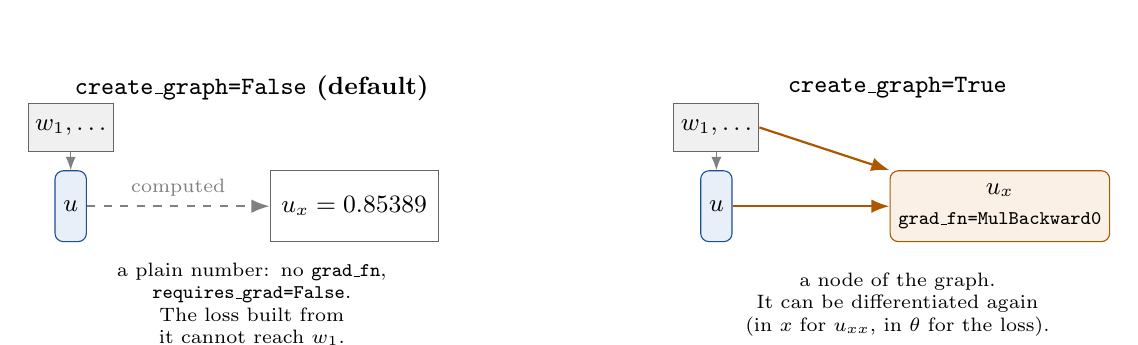
\begin{tikzpicture}
\begin{scope}
\node[font=\small\bfseries] at (2.3,1.5) {\texttt{create\_graph=False} (default)};
\node[val=fwd] (u) at (0,0) {$u$};
\node[par] (w) at (0,1.0) {$w_1,\ldots$};
\draw[->,black!50] (w) -- (u);
\node[draw=black!60,fill=white,font=\small,minimum height=9mm,inner sep=4pt] (ux) at (3.6,0) {$u_x=0.85389$};
\draw[->,thick,dashed,black!50] (u) -- node[above,font=\scriptsize] {computed} (ux);
\node[font=\scriptsize,align=center,text width=44mm] at (2.3,-1.25) {a plain number: no \texttt{grad\_fn},\\\texttt{requires\_grad=False}.\\The loss built from it cannot reach $w_1$.};
\end{scope}
\begin{scope}[xshift=8.2cm]
\node[font=\small\bfseries] at (2.3,1.5) {\texttt{create\_graph=True}};
\node[val=fwd] (u) at (0,0) {$u$};
\node[par] (w) at (0,1.0) {$w_1,\ldots$};
\draw[->,black!50] (w) -- (u);
\node[val=der] (ux) at (3.6,0) {$u_x$\\{\scriptsize \texttt{grad\_fn=MulBackward0}}};
\draw[eg=der] (u) -- (ux);
\draw[eg=der] (w.east) -- (ux.north west);
\node[font=\scriptsize,align=center,text width=44mm] at (2.3,-1.25) {a node of the graph.\\It can be differentiated again\\(in $x$ for $u_{xx}$, in $\theta$ for the loss).};
\end{scope}
\end{tikzpicture}
\end{center}
\texttt{create\_graph}가 없으면 $u_x$는 그래프와 끊긴 텐서이고, 이를 다시 미분하면
\begin{lstlisting}[language={},numbers=none]
RuntimeError: element 0 of tensors does not require grad and does not have a grad_fn
\end{lstlisting}
오류가 난다 (\texttt{autograd\_tiny.py}의 6번 셀).

\subsection{점이 여러 개일 때: \texttt{grad\_outputs=torch.ones\_like(u)}}

collocation point $N$개를 한 번에 넣으면 \texttt{x}와 \texttt{u}의 모양은 $(N,1)$이다.
\texttt{u}가 벡터이면 \texttt{grad\_outputs=v}를 주어야 하고, 이때 \texttt{autograd.grad}는 \textbf{벡터--야코비 곱} $\vect v\T J$, $J_{ij}=\partial u_i/\partial x_j$를 계산한다.

각 샘플은 독립적으로 계산되므로 $u_i$는 $x_i$에만 의존한다. 즉 $J$는 대각행렬이고, $\vect v=(1,\ldots,1)$이면
\[
(\vect v\T J)_j=\sum_i \pd{u_i}{x_j}=\pd{u_j}{x_j},
\]
점마다의 도함수가 된다. \texttt{autograd\_tiny.py}의 7번 셀에서 점 $3$개로 확인한 결과:
\begin{center}
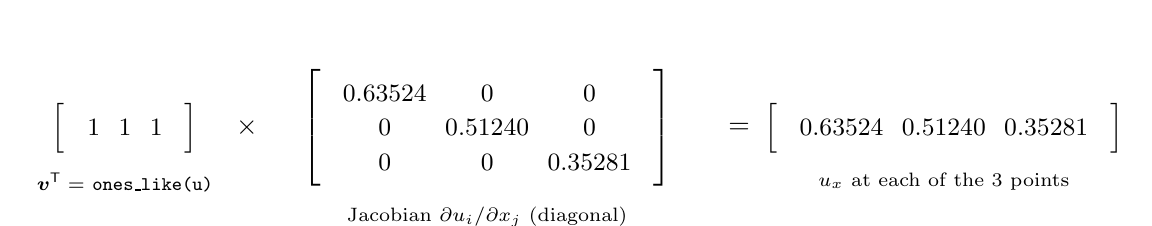
\begin{tikzpicture}
\matrix (v) [matrix of math nodes,left delimiter={[},right delimiter={]},nodes={font=\small}] at (0,0) {1 & 1 & 1\\};
\matrix (J) [matrix of math nodes,left delimiter={[},right delimiter={]},nodes={font=\small,minimum width=13mm}] at (4.6,0)
{0.63524 & 0 & 0\\ 0 & 0.51240 & 0\\ 0 & 0 & 0.35281\\};
\node at (1.55,0) {$\times$};
\node at (7.8,0) {$=$};
\matrix (r) [matrix of math nodes,left delimiter={[},right delimiter={]},nodes={font=\small}] at (10.4,0) {0.63524 & 0.51240 & 0.35281\\};
\node[font=\scriptsize,below=1mm of v] {$\vect v\T=$ \texttt{ones\_like(u)}};
\node[font=\scriptsize,below=1mm of J] {Jacobian $\partial u_i/\partial x_j$ (diagonal)};
\node[font=\scriptsize,below=1mm of r] {$u_x$ at each of the 3 points};
\end{tikzpicture}
\end{center}
따라서 PINN 코드에는 다음 함수가 쓰인다.
\begin{lstlisting}
def derivative(y, x):
    return torch.autograd.grad(y, x, grad_outputs=torch.ones_like(y), create_graph=True)[0]
\end{lstlisting}

\begin{thinkbox}[이 방법이 틀리는 경우]
BatchNorm처럼 미니배치의 샘플을 섞는 층이 있으면 $J$가 대각이 아니고, 위의 합은 $\partial u_j/\partial x_j$가 아니다.
PINN에 BatchNorm을 쓰지 않는 이유 중 하나이다.
\end{thinkbox}

% =================================================
\section{첫 번째 PINN: 1차원 Poisson 방정식}\label{sec:poisson}
% =================================================

식 \eqref{eq:poisson}을 푼다 (\texttt{pinn\_poisson\_1d.py}).

\subsection{구조}

\begin{center}
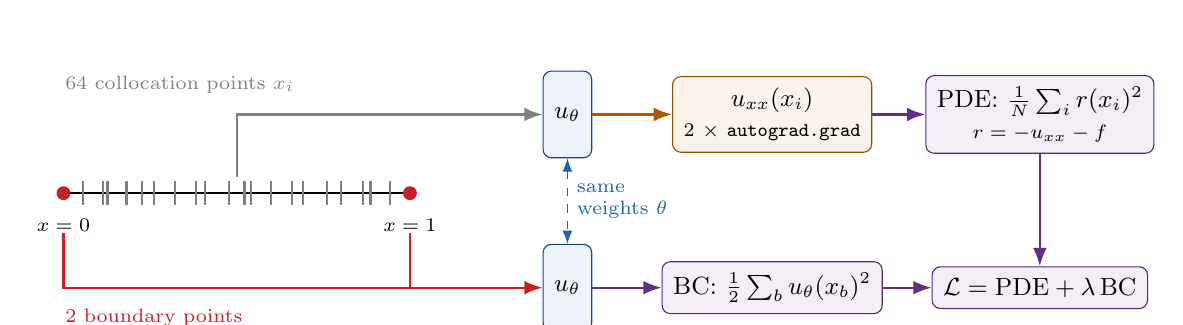
\begin{tikzpicture}
% the interval
\draw[thick] (0,0) -- (4.4,0);
\foreach \t in {0.25,0.5,0.56,0.8,1.0,1.15,1.42,1.68,1.8,2.1,2.3,2.38,2.64,2.9,3.04,3.35,3.52,3.8,3.9,4.15} \draw[gray,thick] (\t,-0.15) -- (\t,0.15);
\fill[bwd] (0,0) circle (2.5pt); \fill[bwd] (4.4,0) circle (2.5pt);
\node[below,font=\scriptsize] at (0,-0.2) {$x=0$}; \node[below,font=\scriptsize] at (4.4,-0.2) {$x=1$};
\node[font=\scriptsize,gray,anchor=south west] at (-0.1,1.15) {64 collocation points $x_i$};
\node[font=\scriptsize,bwd,anchor=north west] at (-0.1,-1.35) {2 boundary points};
% one network, two kinds of inputs
\node[box=fwd,minimum height=11mm] (n1) at (6.4,1.0) {$u_\theta$};
\node[box=fwd,minimum height=11mm] (n2) at (6.4,-1.2) {$u_\theta$};
\draw[<->,dashed,fwd] (n1) -- node[right,font=\scriptsize,align=left] {same\\weights $\theta$} (n2);
\draw[->,thick,gray] (2.2,0.2) |- (n1.west);
\draw[->,thick,bwd] (0,-0.5) |- (n2.west);
\draw[thick,bwd] (4.4,-0.5) -- (4.4,-1.2);
\node[box=der] (d) at (9.0,1.0) {$u_{xx}(x_i)$\\{\scriptsize 2 $\times$ \texttt{autograd.grad}}};
\node[box=lossc] (lp) at (12.4,1.0) {PDE: $\frac1N\sum_i r(x_i)^2$\\{\scriptsize $r=-u_{xx}-f$}};
\node[box=lossc] (lb) at (9.0,-1.2) {BC: $\frac12\sum_{b}u_\theta(x_b)^2$};
\node[box=lossc] (L) at (12.4,-1.2) {$\loss=\text{PDE}+\lambda\,\text{BC}$};
\draw[eg=der] (n1) -- (d); \draw[eg=lossc] (d) -- (lp);
\draw[eg=lossc] (n2) -- (lb);
\draw[eg=lossc] (lp) -- (L);
\draw[eg=lossc] (lb) -- (L);
\end{tikzpicture}

\small 같은 신경망 (같은 가중치)에 두 종류의 점을 넣는다. collocation point에서는 미분 그래프를 거쳐 residual을, 경계에서는 값 자체를 본다.
\end{center}

\subsection{최소한의 코드}

PINN으로 1차원 poisson 문제를 푸는 코드는 다음과 같다 (\texttt{pinn\_poisson\_1d\_simple.py}).
\begin{lstlisting}
torch.manual_seed(0)
device = "cuda" if torch.cuda.is_available() else "cpu"

# network u_theta: R -> R, smooth activation (tanh) so that u'' exists
model = nn.Sequential(nn.Linear(1, 32),
                      nn.Tanh(),
                      nn.Linear(32, 32),
                      nn.Tanh(),
                      nn.Linear(32, 32),
                      nn.Tanh(),
                      nn.Linear(32, 1)).to(device)

# training points: locations only, no labels
x_f = torch.rand(64, 1, device=device, requires_grad=True)     # collocation points in (0, 1): (64, 1)
x_b = torch.tensor([[0.0], [1.0]], device=device)              # boundary points: (2, 1)

optimizer = torch.optim.Adam(model.parameters(), lr=1e-3)
for step in range(5000):
    u    = model(x_f)                                                                              
    u_x  = torch.autograd.grad(u,   x_f, grad_outputs=torch.ones_like(u),   create_graph=True)[0]  
    u_xx = torch.autograd.grad(u_x, x_f, grad_outputs=torch.ones_like(u_x), create_graph=True)[0]  
    r    = -u_xx - math.pi**2 * torch.sin(math.pi * x_f)                                          

    loss = torch.mean(r**2) + torch.mean(model(x_b)**2)        # PDE term + boundary term (u(0) = u(1) = 0)

    optimizer.zero_grad()
    loss.backward()            # d(loss)/d(theta), through the original and the derivative graphs
    optimizer.step()

# compare with the exact solution (used only here, never in training)
x = torch.linspace(0, 1, 1001, device=device).reshape(-1, 1)
with torch.no_grad():
    u_pred = model(x)
u_true = torch.sin(math.pi * x)
print("relative L2 error:", (torch.norm(u_pred - u_true) / torch.norm(u_true)).item())
\end{lstlisting}
학습 루프의 처음 네 줄이 \ref{sec:onestep}절의 1--2단계 (forward와 입력에 대한 미분)이고, \texttt{loss}가 3단계,
\texttt{loss.backward()}와 \texttt{optimizer.step()}이 4--5단계이다. 정확한 해 $u^*$는 마지막 오차 계산에만 쓰인다.
상대오차는 $6.1\times10^{-5}$이다.

\subsection{기능을 더한 코드}

\texttt{pinn\_poisson\_1d.py}는 위 코드와 같은 계산을 한다 (seed와 설정이 같아 상대오차도 $6.128\times10^{-5}$로 같다).
네 부분으로 나누어 읽는다 (유한차분법과 비교하는 182--193줄은 생략). 줄 번호는 파일의 줄 번호이다.

\paragraph{설정, 문제, 신경망, 학습에 쓸 점 (1--58줄).}
\lstinputlisting[firstline=1,lastline=58,firstnumber=1]{code/pinn_poisson_1d.py}
23줄은 GPU가 있으면 GPU를 쓴다. 27--31줄은 우변 $f$와, 오차를 잴 때만 쓰는 정확한 해 $u^*$이다.
33--46줄의 \texttt{MLP}는 최소한의 코드의 \texttt{nn.Sequential}과 같은 신경망 (은닉층 $3$개, 각 $32$개 뉴런, $\tanh$, 매개변수 $2209$개)을
\texttt{depth}와 \texttt{width}로 만든다.
\texttt{requires\_grad}는 collocation point \texttt{x\_f}에만 켠다 (55줄). 경계점 \texttt{x\_b} (56줄)에서는 미분하지 않는다.

\paragraph{residual, loss, 학습 (59--121줄).}
\lstinputlisting[firstline=59,lastline=121,firstnumber=59]{code/pinn_poisson_1d.py}
60--64줄의 \texttt{derivative}는 \texttt{autograd.grad} 한 줄을 함수로 묶은 것이고,
66--70줄의 \texttt{residual}은 \ref{sec:graph}절의 그래프 (원래 그래프 $\to u_x\to u_{xx}\to r$)를 그대로 따른다.
75--79줄의 \texttt{loss\_terms}는 식 \eqref{eq:pinnloss}의 두 항을 따로 돌려준다. 경계 항은 평균이므로 $\frac12(u(0)^2+u(1)^2)$이고, 73줄의 \texttt{lam\_b}가 $\lambda$이다.
학습 루프 (97--118줄)에서 104--108줄은 최소한의 코드의 루프와 같다. \ref{sec:onestep}절의 1--3단계가 105--106줄 (\texttt{loss\_terms} 안), 4단계가 107줄, 5단계가 108줄이다.
나머지는 기록이다. 98--100줄은 \texttt{snap\_steps}의 step에서 해를 저장하고 (아래 학습 중의 해 그림), 110--115줄은 $50$ step마다 loss의 각 항과 상대오차 (83--87줄)를 기록한다.

\paragraph{그림 (122--165줄).}
\lstinputlisting[firstline=122,lastline=165,firstnumber=122]{code/pinn_poisson_1d.py}
127--128줄은 collocation point가 아닌 $1001$개 점에서 residual을 계산한다 (결과 그림 (d)). 이 점들로 다시 미분하므로 \texttt{requires\_grad}를 켠다.

\paragraph{L-BFGS (166--180줄).}
\lstinputlisting[firstline=166,lastline=180,firstnumber=166]{code/pinn_poisson_1d.py}
Adam으로 학습한 신경망을 L-BFGS로 이어서 학습한다. L-BFGS는 한 step에 loss를 여러 번 계산하므로 169--174줄의 \texttt{closure}를 넘긴다.

\subsection{결과}

Adam으로 $5000$ step 학습하는 데 GPU (RTX 3050)에서 약 $40$초가 걸렸다.

\begin{center}
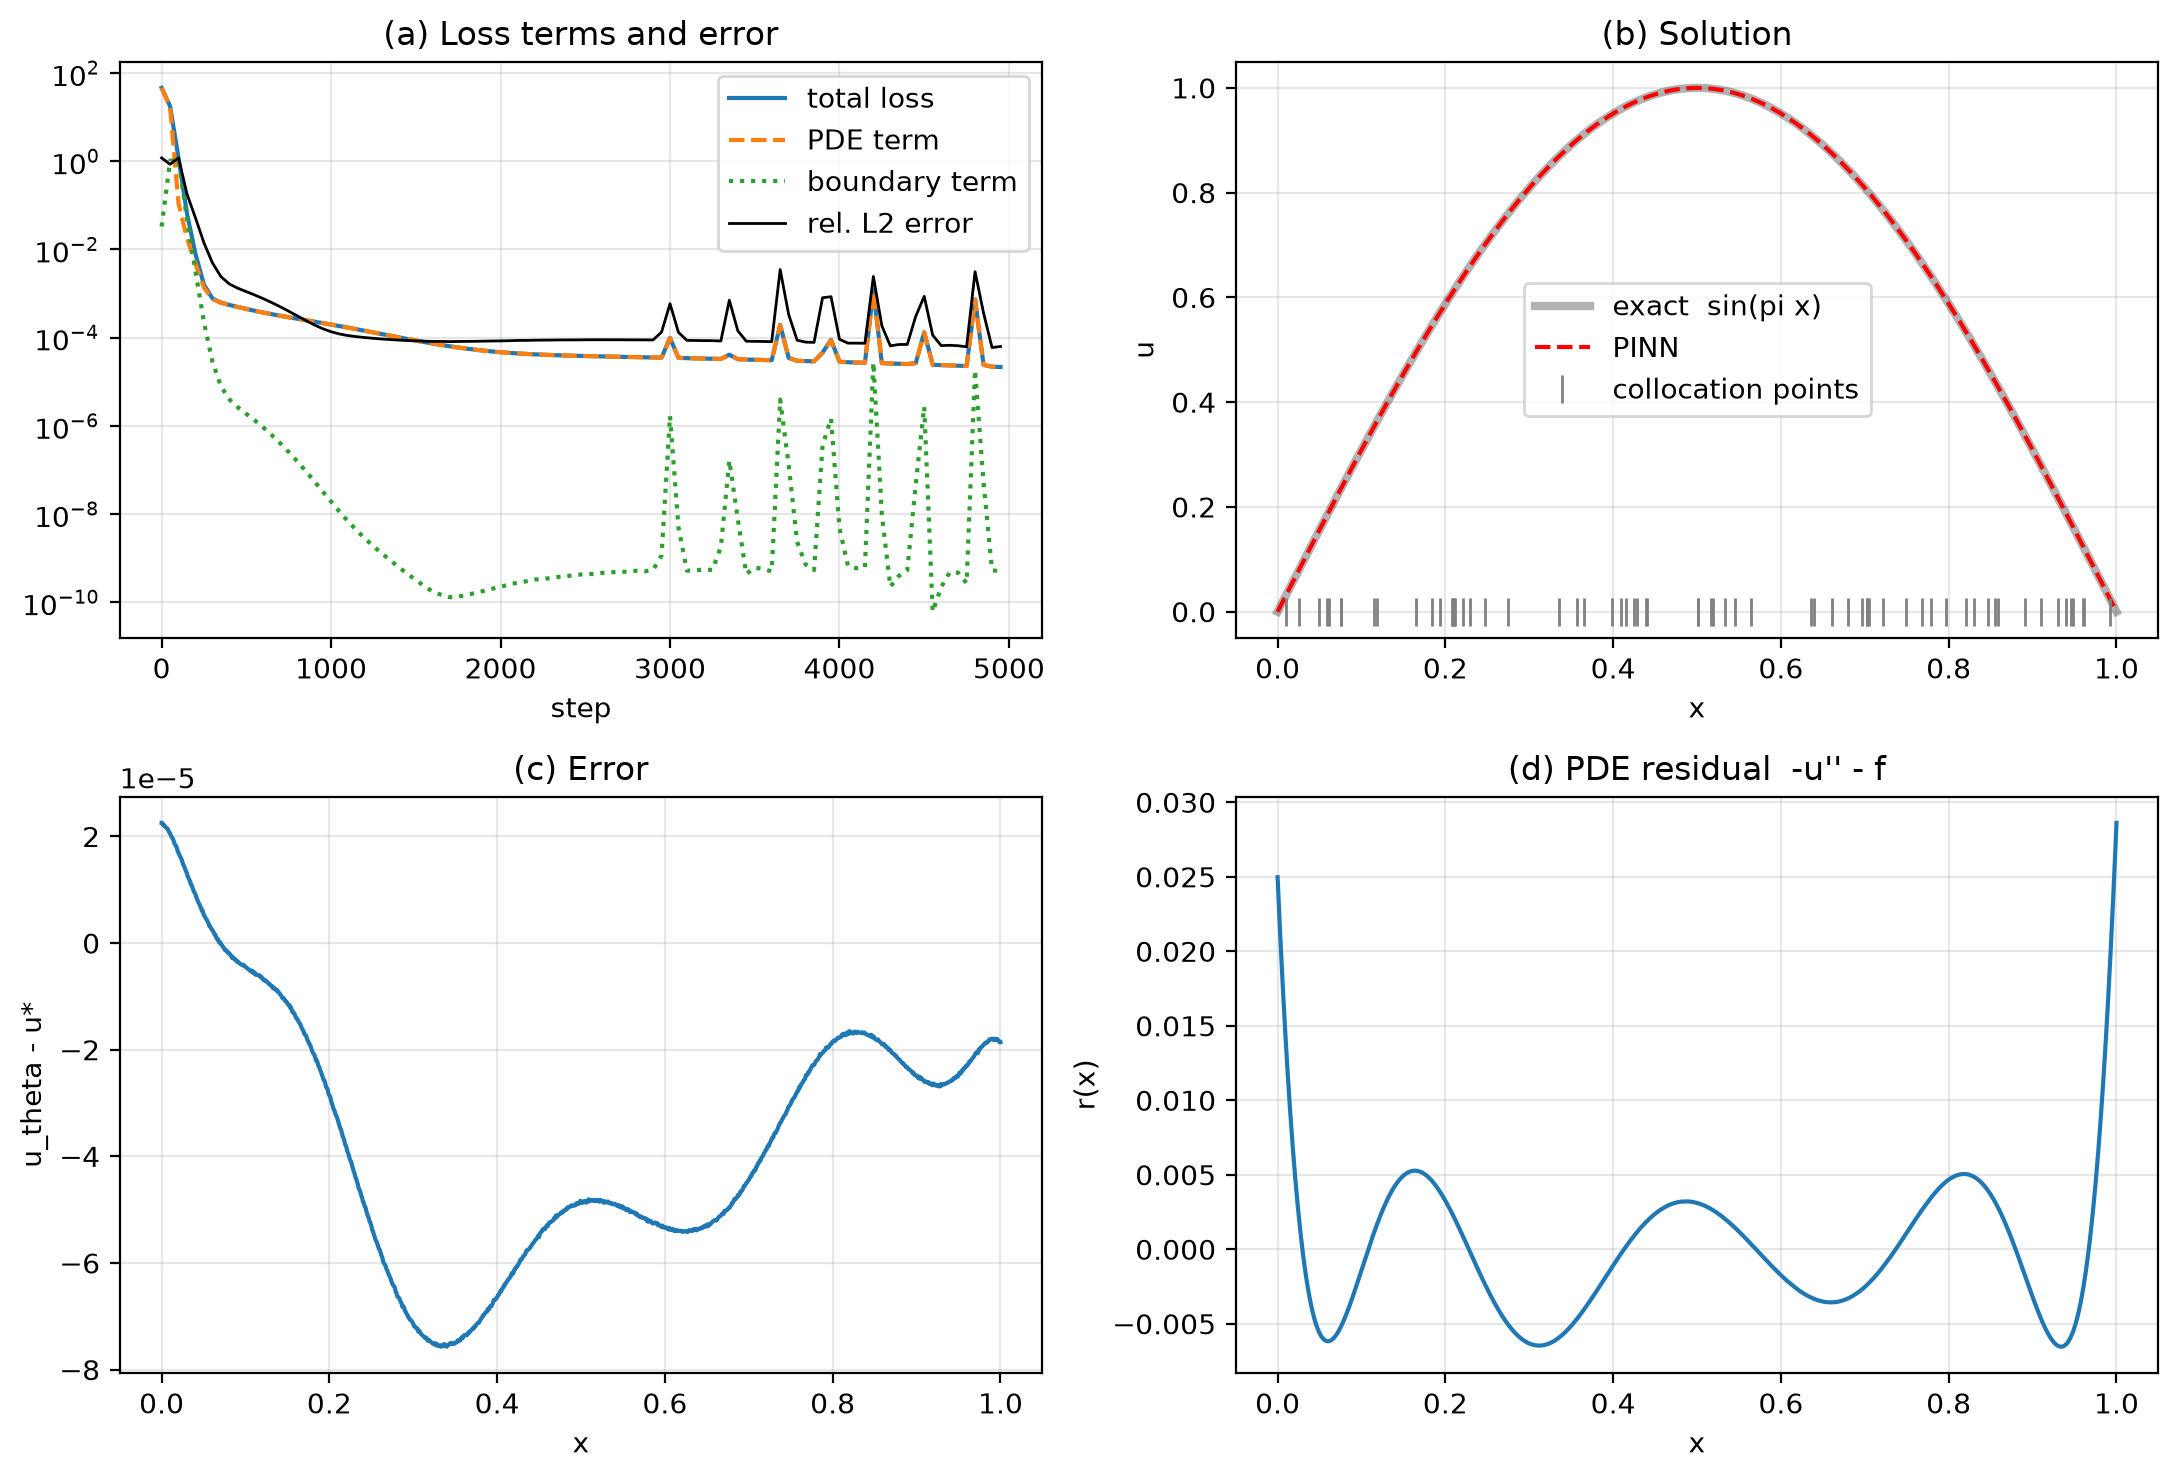
\includegraphics[width=\textwidth]{figures/poisson_result.png}

\small (a) loss의 각 항과 상대오차, (b) PINN의 해와 정확한 해, (c) 오차 $u_\theta-u^*$, (d) $[0,1]$ 전체에서 계산한 residual.
\end{center}

\begin{itemize}[leftmargin=1.5em]
\item 처음 loss $46.2$는 거의 PDE 항이다. 초기 신경망은 거의 상수여서 $u''\approx0$, $r\approx-f$이고,
PDE 항은 $\int_0^1f^2\,dx=\pi^4/2\approx48.7$에 가깝다.
\item 상대오차는 $1000$ step에서 $1.4\times10^{-4}$, $5000$ step에서 $6.1\times10^{-5}$이다.
(a)처럼 $3000$ step 이후 loss가 간헐적으로 튄다 (Adam에서 흔하다).
\item (b)에서 두 해는 구별되지 않으며, (c)의 오차는 $10^{-5}$ 크기이다.
\item (d)는 $[0,1]$의 $1001$개 점에서 계산한 residual이다. loss에는 collocation point $64$개의 residual만 들어가므로 그 사이의 residual은 보장되지 않지만,
여기서는 전 구간에서 $0.03$ 이하이며 양 끝 근처에서 가장 크다.
\end{itemize}

\begin{center}
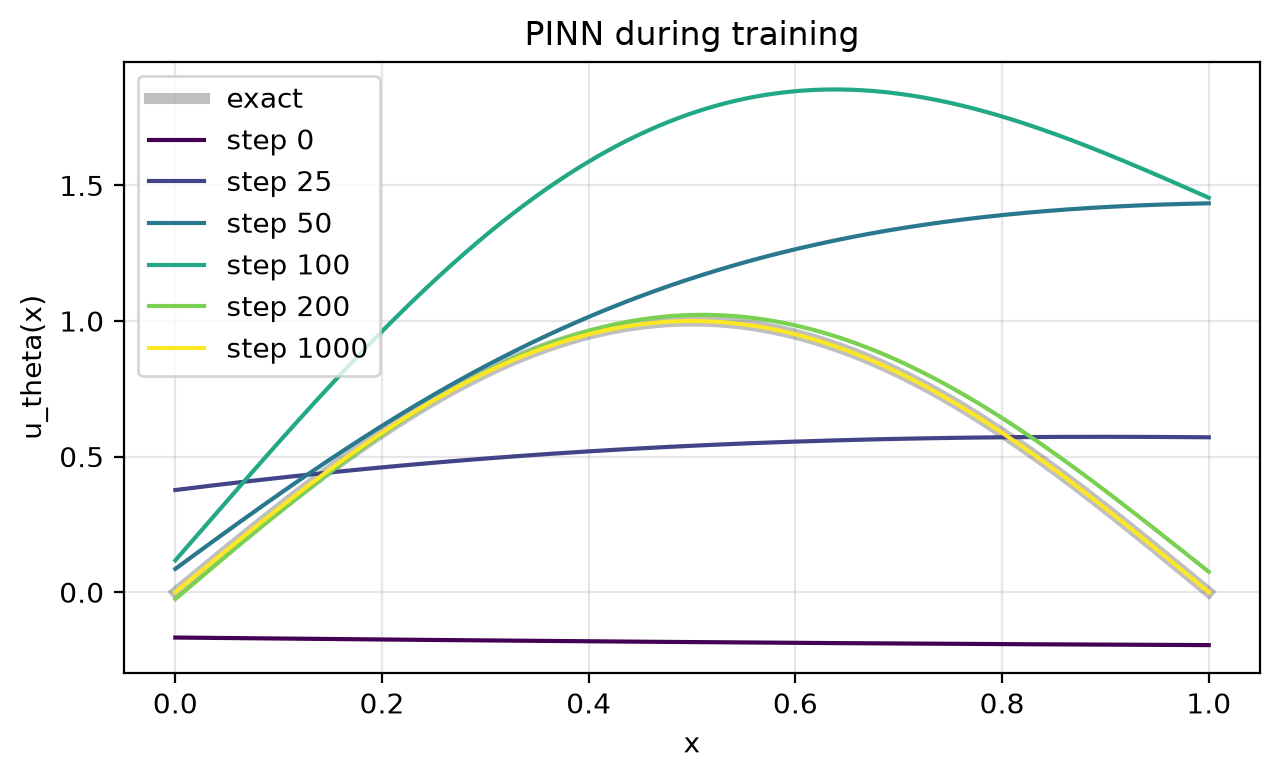
\includegraphics[width=0.72\textwidth]{figures/poisson_snapshots.png}

\small 학습 중의 $u_\theta(x)$. 곡률 (모양)이 먼저 맞고, 경계값은 나중에 맞는다.
\end{center}

$100$ step의 곡선은 위로 볼록하지만 기울어져 있어 $u(1)\approx1.45$이고, $200$ step에서 양 끝이 $0$ 근처로 내려온다.
$-u''=f$의 일반해는 특수해에 $c_0+c_1x$를 더한 것이므로, PDE 항은 $c_0$, $c_1$을 정하지 못한다. 이 두 자유도는 경계 항이 정한다.
초기에는 PDE 항이 훨씬 크므로 곡률이 먼저 맞고, $c_0$, $c_1$은 나중에 맞는다.

\begin{remarkbox}[L-BFGS로 마무리하기]
PINN에서는 Adam 뒤에 \textbf{L-BFGS}로 마무리하는 경우가 많다.
L-BFGS는 Newton 방법의 Hessian을 최근 gradient들로 근사하는 준-Newton 방법으로, 최솟값 근처에서 빠르게 수렴한다.
미니배치가 없어 loss가 결정적인 PINN에 적합하다. 166--180줄에서 L-BFGS를 이어서 돌리면 $1$초 이내에 loss가 $2.1\times10^{-6}$,
상대오차가 $1.5\times10^{-5}$로 줄었다. L-BFGS는 한 step에 loss를 여러 번 계산하므로 \texttt{closure}를 넘긴다.
\end{remarkbox}

\begin{keybox}[중간 정리]
\begin{itemize}[leftmargin=1.5em]
\item PINN은 신경망 $u_\theta$를 해의 후보로 두고, 방정식의 residual과 경계조건의 오차를 loss로 최소화한다. 정답 데이터가 필요 없다.
\item $u_x$, $u_{xx}$는 \texttt{torch.autograd.grad(..., create\_graph=True)}로 구한다. 이 계산은 원래 그래프의 노드를 재료로 쓰는 \textbf{미분 그래프}를 만든다.
\item residual이 원래 그래프와 미분 그래프를 하나로 잇고, \texttt{loss.backward()}는 그 전체를 거꾸로 지나간다.
한 가중치가 여러 곳에 있으면 경로마다의 기여가 \textbf{더해진다}.
\item 활성화 함수는 매끄러워야 한다 ($\tanh$). ReLU는 $u''=0$이 되어 조용히 실패한다.
\item \texttt{grad\_outputs=ones\_like(u)}는 샘플끼리 독립이어서 야코비가 대각이기 때문에 점마다의 도함수를 준다.
\end{itemize}
\end{keybox}

% =================================================
\section{시간이 있는 문제: 열 방정식}\label{sec:heat}
% =================================================

\subsection{편미분방정식과 열 방정식}

미지 함수가 둘 이상의 변수의 함수이고 방정식에 편도함수가 들어가면 \textbf{편미분방정식 (PDE)}이라 한다.
길이 $1$인 막대의 온도 $u(x,t)$ (위치 $x$, 시각 $t$)는 1차원 \textbf{열 방정식}을 만족한다.
\begin{equation}\label{eq:heat}
u_t=\kappa\,u_{xx}\quad(0<x<1,\ 0<t<1),\qquad u(x,0)=\sin(\pi x),\qquad u(0,t)=u(1,t)=0.
\end{equation}
$u_t=\partial u/\partial t$, $u_{xx}=\partial^2u/\partial x^2$이고, $\kappa>0$은 열확산계수이다 (여기서는 $\kappa=0.1$).
해를 정하려면 $t=0$에서의 \textbf{초기조건}과 양 끝의 \textbf{경계조건}이 모두 필요하다.
$u=X(x)T(t)$를 대입하면 $T'/(\kappa T)=X''/X$이고, 양변이 상수 $-\pi^2$일 때 초기조건과 경계조건을 만족한다. 따라서
\[
u^*(x,t)=e^{-\kappa\pi^2t}\sin(\pi x).
\]
공간 모양은 그대로이고 진폭이 지수적으로 감소한다 ($t=1$에서 $e^{-0.1\pi^2}\approx0.37$배).

PINN에서 Poisson 문제와 다른 점은 두 가지이다.
\begin{enumerate}[leftmargin=1.8em]
\item 신경망의 입력이 $(x,t)$ \textbf{두 개}이다: $u_\theta:\R^2\to\R$.
\item 조건이 세 종류이다: 방정식 (내부), \textbf{초기조건} ($t=0$), 경계조건 ($x=0,1$). 그래서 loss의 항도 세 개이다.
\end{enumerate}

\subsection{입력이 두 개일 때의 미분}\label{sec:twoinputs}

입력을 한 텐서 \texttt{X}에 모아 모양 $(N,2)$로 만든다. 첫 번째 열이 $x$, 두 번째 열이 $t$이다.
\texttt{u}를 \texttt{X}로 미분하면 결과는 \texttt{X}와 같은 모양 $(N,2)$이며, 각 행은 그 점에서의 기울기 $(u_x,u_t)$이다.
$u_{xx}$를 얻으려면 $u_x$ 열을 다시 \texttt{X}로 미분하고 첫 번째 열을 가져온다.

\begin{center}
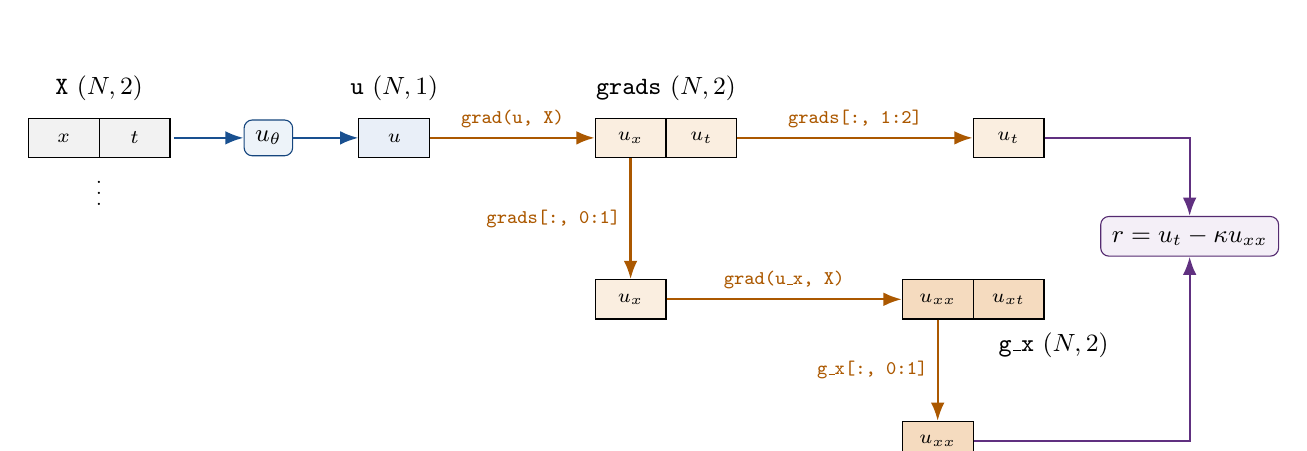
\begin{tikzpicture}[mat/.style={draw,minimum width=9mm,minimum height=5mm,font=\scriptsize,inner sep=1pt}]
% X
\node[mat,fill=black!5] (X1) at (0,0.25) {$x$}; \node[mat,fill=black!5] (X2) at (0.9,0.25) {$t$};
\node[font=\scriptsize] at (0.45,-0.35) {$\vdots$};
\node[font=\small,above] at (0.45,0.6) {\texttt{X} $(N,2)$};
% network
\node[box=fwd] (n) at (2.6,0.25) {$u_\theta$};
\draw[eg=fwd] (1.4,0.25) -- (n);
\node[mat,fill=fwd!10] (u) at (4.2,0.25) {$u$};
\node[font=\small,above] at (4.2,0.6) {\texttt{u} $(N,1)$};
\draw[eg=fwd] (n) -- (u);
% grad
\node[mat,fill=der!12] (g1) at (7.2,0.25) {$u_x$}; \node[mat,fill=der!12] (g2) at (8.1,0.25) {$u_t$};
\node[font=\small,above] at (7.65,0.6) {\texttt{grads} $(N,2)$};
\draw[eg=der] (u) -- node[above,font=\scriptsize] {\texttt{grad(u, X)}} (g1);
% split
\node[mat,fill=der!12] (ux) at (7.2,-1.8) {$u_x$};
\node[mat,fill=der!12] (ut) at (12.0,0.25) {$u_t$};
\draw[eg=der] (g1.south) -- node[left,font=\scriptsize] {\texttt{grads[:, 0:1]}} (ux.north);
\draw[eg=der] (g2.east) -- node[above,font=\scriptsize] {\texttt{grads[:, 1:2]}} (ut.west);
% second derivative
\node[mat,fill=der!25] (h1) at (11.1,-1.8) {$u_{xx}$}; \node[mat,fill=der!25] (h2) at (12.0,-1.8) {$u_{xt}$};
\node[font=\small,anchor=north west] at (11.75,-2.1) {\texttt{g\_x} $(N,2)$};
\draw[eg=der] (ux.east) -- node[above,font=\scriptsize] {\texttt{grad(u\_x, X)}} (h1.west);
\node[mat,fill=der!25] (uxx) at (11.1,-3.6) {$u_{xx}$};
\draw[eg=der] (h1.south) -- node[left,font=\scriptsize] {\texttt{g\_x[:, 0:1]}} (uxx.north);
\node[box=lossc] (r) at (14.3,-1.0) {$r=u_t-\kappa u_{xx}$};
\draw[eg=lossc] (ut.east) -| (r.north);
\draw[eg=lossc] (uxx.east) -| (r.south);
\end{tikzpicture}

\small 입력이 $(x,t)$일 때. \texttt{grad}는 입력 텐서와 같은 모양을 돌려주므로, 필요한 열을 잘라 쓴다.
$u_{xt}$도 함께 계산되지만 쓰지 않는다.
\end{center}

\begin{lstlisting}
def residual(model, X):
    u = model(X)                                     # (N, 1)
    # derivative with respect to both inputs: (N, 2), the columns are [u_x, u_t]
    grads = torch.autograd.grad(u, X, torch.ones_like(u), create_graph=True)[0]
    u_x, u_t = grads[:, 0:1], grads[:, 1:2]          # (N, 1) each
    # differentiate u_x again: (N, 2) = [u_xx, u_xt]; keep the first column
    g_x = torch.autograd.grad(u_x, X, torch.ones_like(u_x), create_graph=True)[0]
    u_xx = g_x[:, 0:1]
    return u_t - kappa * u_xx
\end{lstlisting}
\texttt{grads[:, 0]} 대신 \texttt{grads[:, 0:1]}로 쓰는 이유는 모양을 $(N,)$이 아닌 $(N,1)$로 유지하기 위해서이다.
\texttt{u\_t}와 \texttt{u\_xx}의 모양이 같아야 \texttt{u\_t - kappa * u\_xx}가 의도대로 계산된다.
($(N,)$과 $(N,1)$을 빼면 broadcasting 때문에 $(N,N)$ 행렬이 되어 버린다.)

\subsection{세 종류의 점과 세 개의 loss 항}

\begin{center}
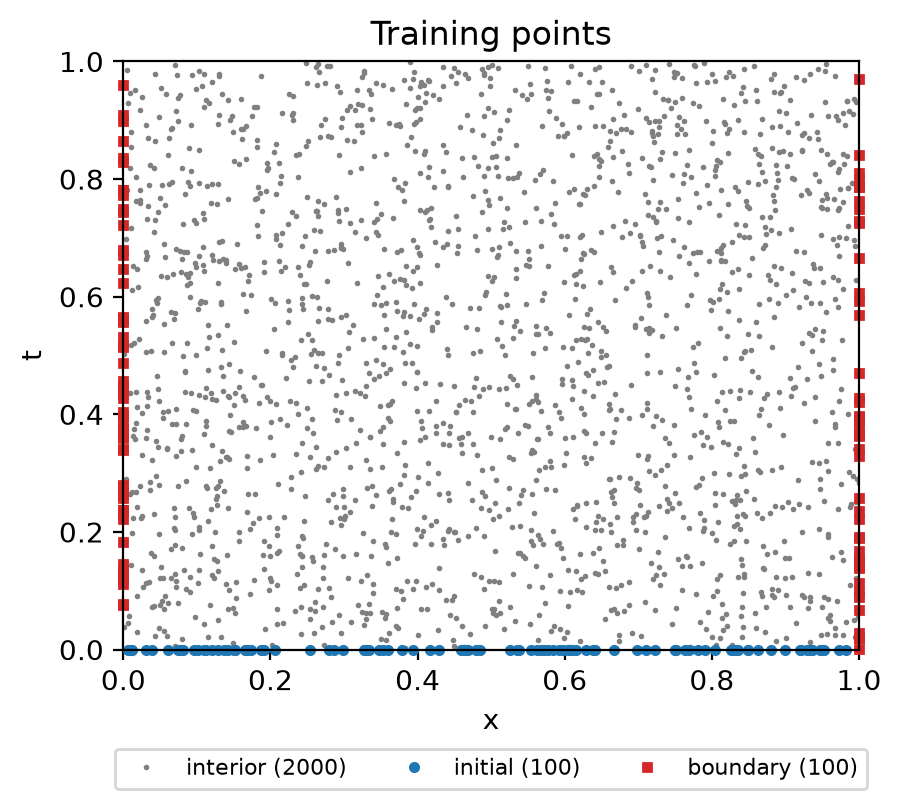
\includegraphics[width=0.45\textwidth]{figures/heat_points.png}

\small 학습에 쓰는 점. 내부 점 $N_f=2000$개, 초기선 ($t=0$) 위의 점 $N_0=100$개, 경계선 ($x=0$, $x=1$) 위의 점 $N_b=100$개를 무작위로 뽑는다.
\end{center}
\[
\loss=\underbrace{\frac1{N_f}\sum_i r(x_i,t_i)^2}_{\text{PDE, interior}}
+\underbrace{\frac1{N_0}\sum_j\big(u_\theta(x_j,0)-\sin\pi x_j\big)^2}_{\text{initial}}
+\underbrace{\frac1{N_b}\sum_k u_\theta(x_k,t_k)^2}_{\text{boundary},\ x_k\in\{0,1\}}
\]
세 항의 가중치는 모두 $1$이다.
세 종류의 점은 같은 신경망을 지난다. PDE 항만 미분 그래프를 거치고, 초기·경계 항은 $u_\theta$의 값만 쓴다.
역전파는 세 항의 gradient를 각 가중치에서 더한다.

\begin{lstlisting}
def loss_terms(model):
    loss_pde = torch.mean(residual(model, X_f)**2)
    loss_ic  = torch.mean((model(X_0) - u_0)**2)
    loss_bc  = torch.mean((model(X_b) - u_b)**2)
    return loss_pde, loss_ic, loss_bc
\end{lstlisting}

\subsection{결과}

신경망은 입력이 $2$개인 것만 빼고 Poisson 문제의 신경망과 같다 ($2\to32\to32\to32\to1$, $\tanh$, 매개변수 $2241$개).
Adam $5000$ step에 GPU (RTX 3050)에서 약 $2$분이 걸렸고, $101\times101$ 격자에서 잰 상대오차는 $1.7\times10^{-3}$,
최대 절대오차는 $6.5\times10^{-3}$이었다.

\begin{center}
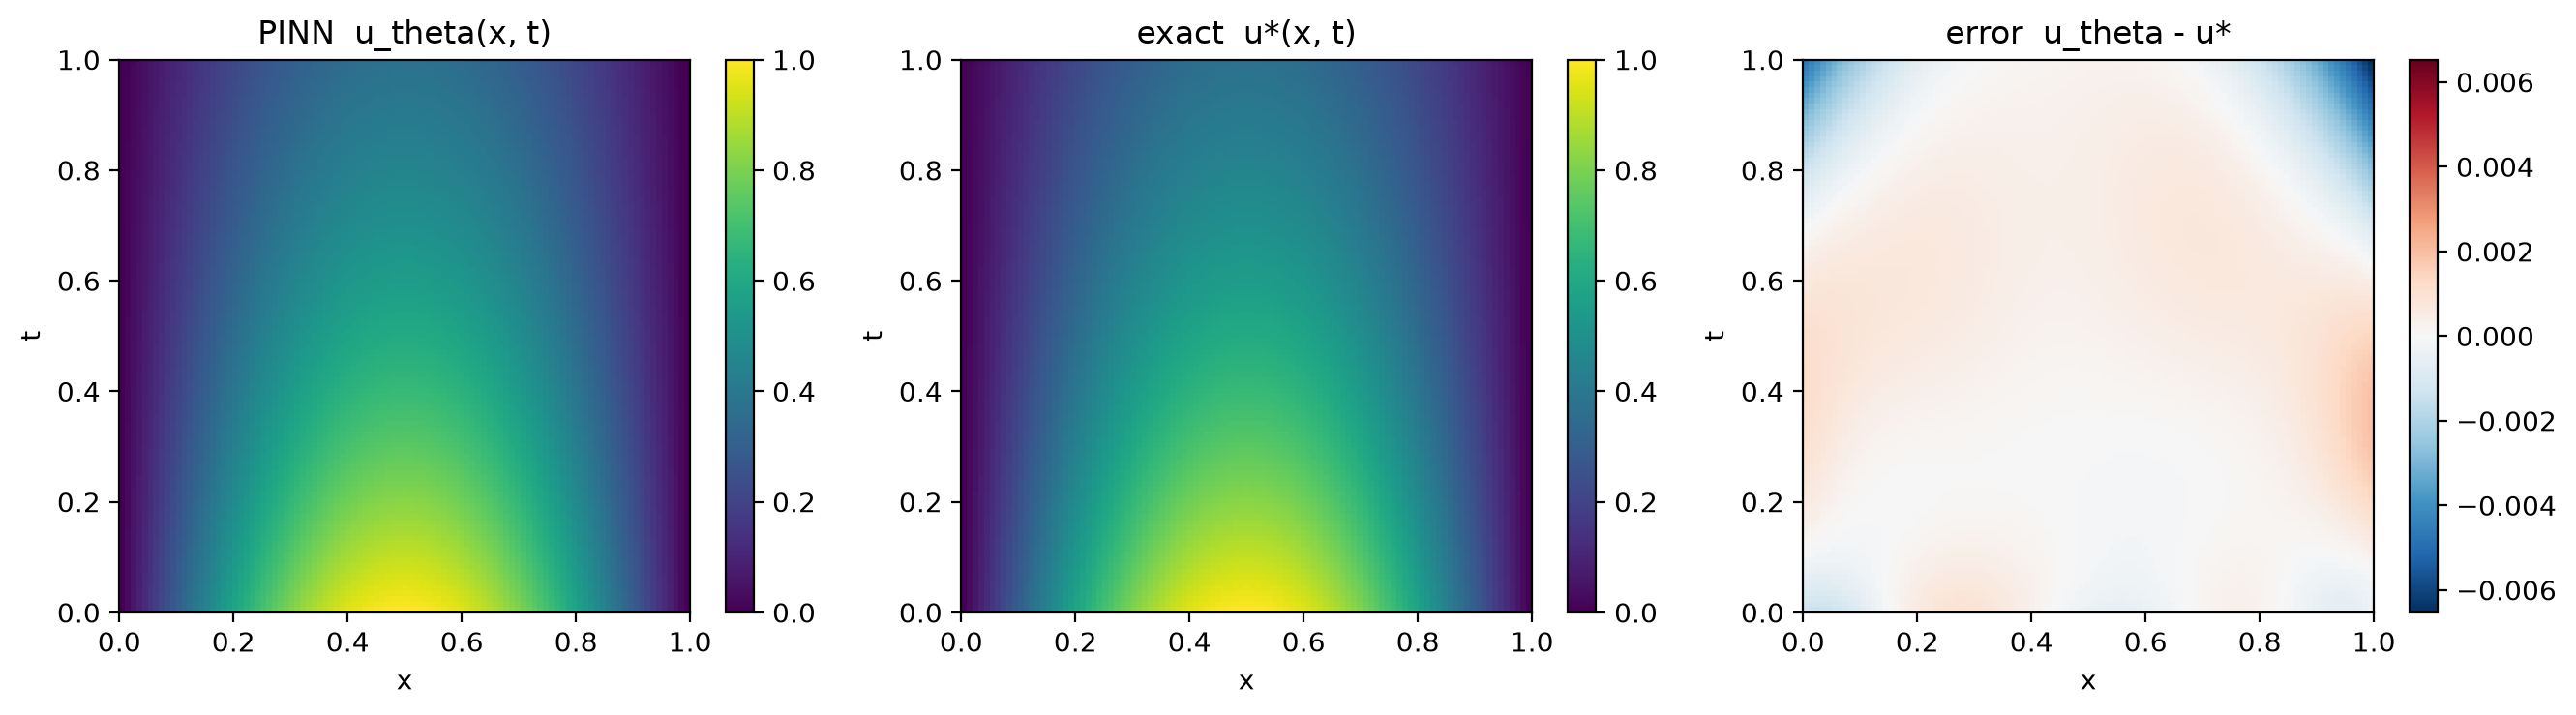
\includegraphics[width=\textwidth]{figures/heat_field.png}

\small 왼쪽부터 PINN의 해, 정확한 해, 오차. 가로축이 $x$, 세로축이 시간 $t$이다.
\end{center}

\begin{center}
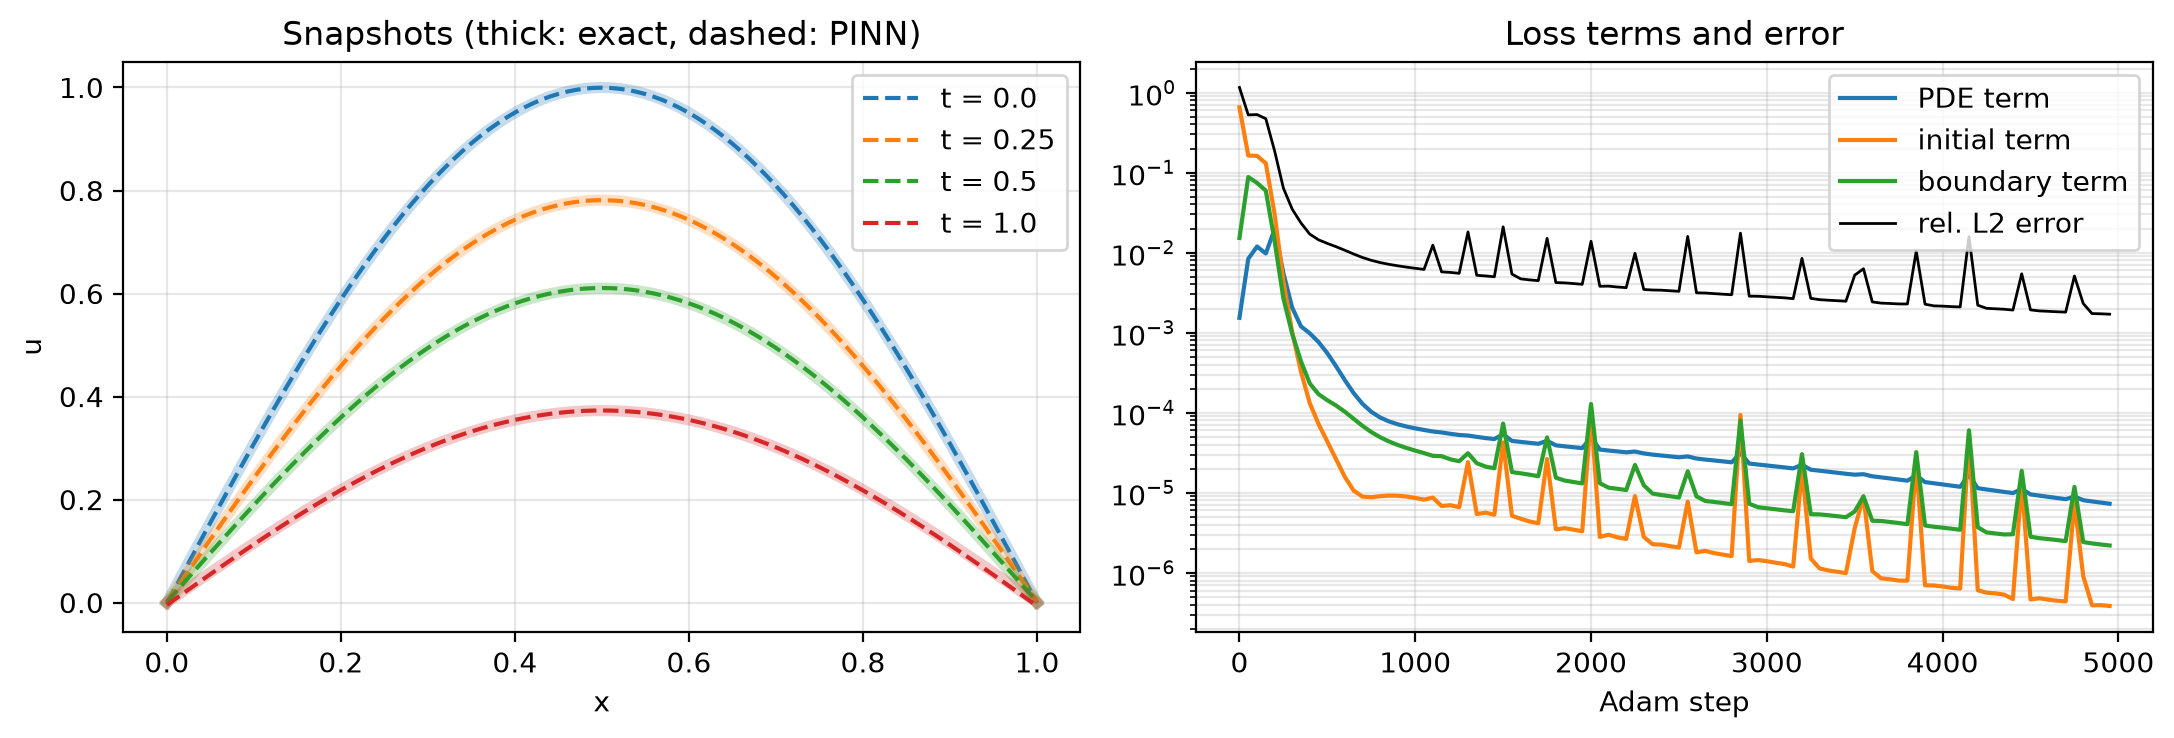
\includegraphics[width=\textwidth]{figures/heat_snapshots.png}

\small 왼쪽: 네 시각에서의 단면 (굵은 선: 정확한 해, 점선: PINN). 오른쪽: loss의 세 항과 상대오차.
\end{center}

\begin{itemize}[leftmargin=1.5em]
\item 처음에 PDE 항은 $1.5\times10^{-3}$, 초기조건 항은 $0.65$이다. 초기 신경망은 거의 상수이고, \textbf{상수 함수는 열 방정식의 해이다} ($u_t=0=\kappa u_{xx}$).
PDE만으로는 해가 유일하지 않으며, 초기조건과 경계조건이 해를 하나로 정한다.
\item 오차는 $t=1$ 근처의 두 모서리 ($x\approx0$, $x\approx1$)에서 가장 크다.
\item Adam의 loss가 주기적으로 튀는 현상은 Poisson 문제에서와 같다.
\end{itemize}

% =================================================
\section{역문제: 측정값에서 계수 찾기}\label{sec:inverse}
% =================================================

\subsection{순문제와 역문제}

방정식, 계수 $\kappa$, 초기·경계조건이 주어졌을 때 해 $u$를 구하는 문제를 \textbf{순문제(forward problem)}라 한다.
반대로 $u$의 측정값으로부터 $\kappa$를 구하는 문제를 \textbf{역문제(inverse problem)}라 한다.

\begin{center}
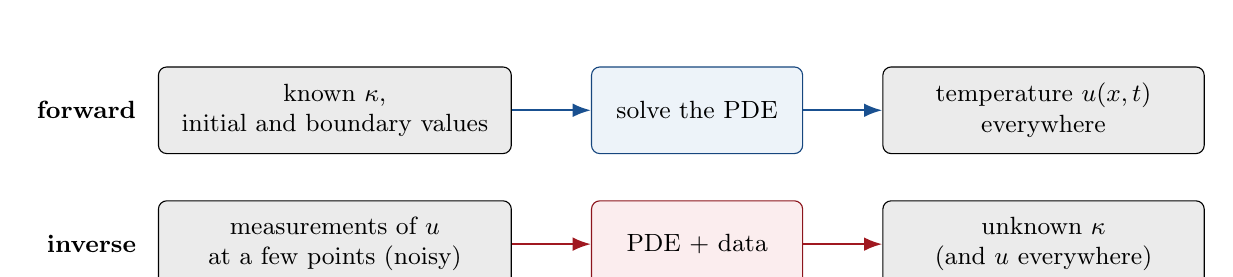
\begin{tikzpicture}
\node[box=black,text width=42mm,minimum height=11mm] (k1) at (0,0) {known $\kappa$,\\initial and boundary values};
\node[box=fwd,text width=24mm,minimum height=11mm] (s1) at (4.6,0) {solve the PDE};
\node[box=black,text width=38mm,minimum height=11mm] (u1) at (9.0,0) {temperature $u(x,t)$\\everywhere};
\draw[eg=fwd] (k1) -- (s1); \draw[eg=fwd] (s1) -- (u1);
\node[font=\small\bfseries,anchor=east] at (-2.4,0) {forward};
\node[box=black,text width=42mm,minimum height=11mm] (u2) at (0,-1.7) {measurements of $u$\\at a few points (noisy)};
\node[box=bwd,text width=24mm,minimum height=11mm] (s2) at (4.6,-1.7) {PDE + data};
\node[box=black,text width=38mm,minimum height=11mm] (k2) at (9.0,-1.7) {unknown $\kappa$\\(and $u$ everywhere)};
\draw[eg=bwd] (u2) -- (s2); \draw[eg=bwd] (s2) -- (k2);
\node[font=\small\bfseries,anchor=east] at (-2.4,-1.7) {inverse};
\end{tikzpicture}
\end{center}

역문제는 CT, 전기 임피던스 단층촬영 (EIT: 경계에서 측정한 전압으로 내부의 전기전도도 분포를 구한다; \ref{sec:eit}절), 지하 탐사, 비파괴 검사 등에서 나타난다.
고전적으로는 $\kappa$를 바꾸어 가며 순문제를 반복해서 푼다. PINN에서는 \textbf{$\kappa$를 신경망의 매개변수와 함께 학습}시킨다.

\subsection{$\kappa$를 학습 가능한 매개변수로}

\begin{lstlisting}
kappa = nn.Parameter(torch.tensor(kappa_init, device=device))   # trainable, like a weight
optimizer = torch.optim.Adam(list(model.parameters()) + [kappa], lr=1e-3)
\end{lstlisting}
초깃값은 참값 $0.1$의 다섯 배인 $0.5$이다.
\texttt{nn.Parameter}는 \texttt{requires\_grad=True}인 텐서이고, optimizer에 넘기면 가중치와 같이 갱신된다.
loss는 측정값 항과 PDE 항이다. 초기·경계조건은 모른다고 가정하여 쓰지 않는다.
\[
\loss(\theta,\kappa)=\underbrace{\frac1{N_d}\sum_{j}\big(u_\theta(x_j,t_j)-u^{\text{obs}}_j\big)^2}_{\text{data}}
+\underbrace{\frac1{N_f}\sum_i\big(u_t-\kappa\,u_{xx}\big)^2\Big|_{(x_i,t_i)}}_{\text{PDE}}.
\]

\begin{center}
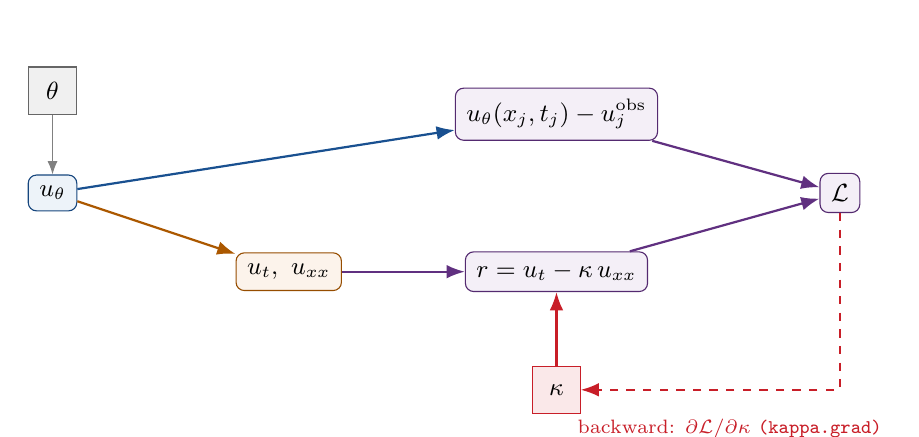
\begin{tikzpicture}
\node[box=fwd] (net) at (0,0) {$u_\theta$};
\node[box=der] (d) at (3.0,-1.0) {$u_t,\ u_{xx}$};
\node[box=lossc] (r) at (6.4,-1.0) {$r=u_t-\kappa\,u_{xx}$};
\node[box=lossc] (dat) at (6.4,1.0) {$u_\theta(x_j,t_j)-u^{\text{obs}}_j$};
\node[box=lossc] (L) at (10.0,0) {$\loss$};
\node[par,fill=bwd!10,draw=bwd] (k) at (6.4,-2.5) {$\kappa$};
\node[par] (th) at (0,1.3) {$\theta$};
\draw[->,black!50] (th) -- (net);
\draw[eg=der] (net) -- (d); \draw[eg=lossc] (d) -- (r); \draw[eg=fwd] (net) -- (dat);
\draw[->,thick,bwd] (k) -- (r);
\draw[eg=lossc] (r) -- (L); \draw[eg=lossc] (dat) -- (L);
\draw[->,dashed,thick,bwd] (L.south) |- (k.east);
\node[font=\scriptsize,bwd,anchor=north] at (8.6,-2.75) {backward: $\partial\loss/\partial\kappa$ \texttt{(kappa.grad)}};
\end{tikzpicture}

\small $\kappa$는 residual에만 들어가는 잎 노드이다. 역전파가 \texttt{kappa.grad}를 채우는 경로는 하나뿐이다.
\end{center}

$\kappa$의 gradient를 손으로 쓰면
\[
\pd{\loss}{\kappa}=\frac{2}{N_f}\sum_i r_i\,\pd{r_i}{\kappa}=\frac{2}{N_f}\sum_i r_i\,(-u_{xx,i}).
\]
측정값 항은 $u_\theta$를 측정값에 맞추고, PDE 항은 그 $u_\theta$가 만족하는 열 방정식의 $\kappa$를 정한다.
$u_\theta$를 고정하면 PDE 항은 $\kappa$의 이차함수이고, $\partial\loss/\partial\kappa=0$에서
\[
\kappa=\frac{\sum_i u_{t,i}\,u_{xx,i}}{\sum_i u_{xx,i}^2},
\]
즉 $u_t$를 $u_{xx}$에 최소제곱으로 회귀한 기울기이다.

\subsection{결과}

측정값 $N_d=200$개, collocation point $N_f=2000$개, Adam $5000$ step이다.
측정값은 $u^*$에 잡음 $\mathcal N(0,\sigma^2)$을 더한 것이고 ($\max u^*=1$이므로 $\sigma=0.05$는 약 $5\%$), 한 번 학습에 GPU (RTX 3050)로 약 $2.5$--$3$분이 걸렸다.

\begin{center}
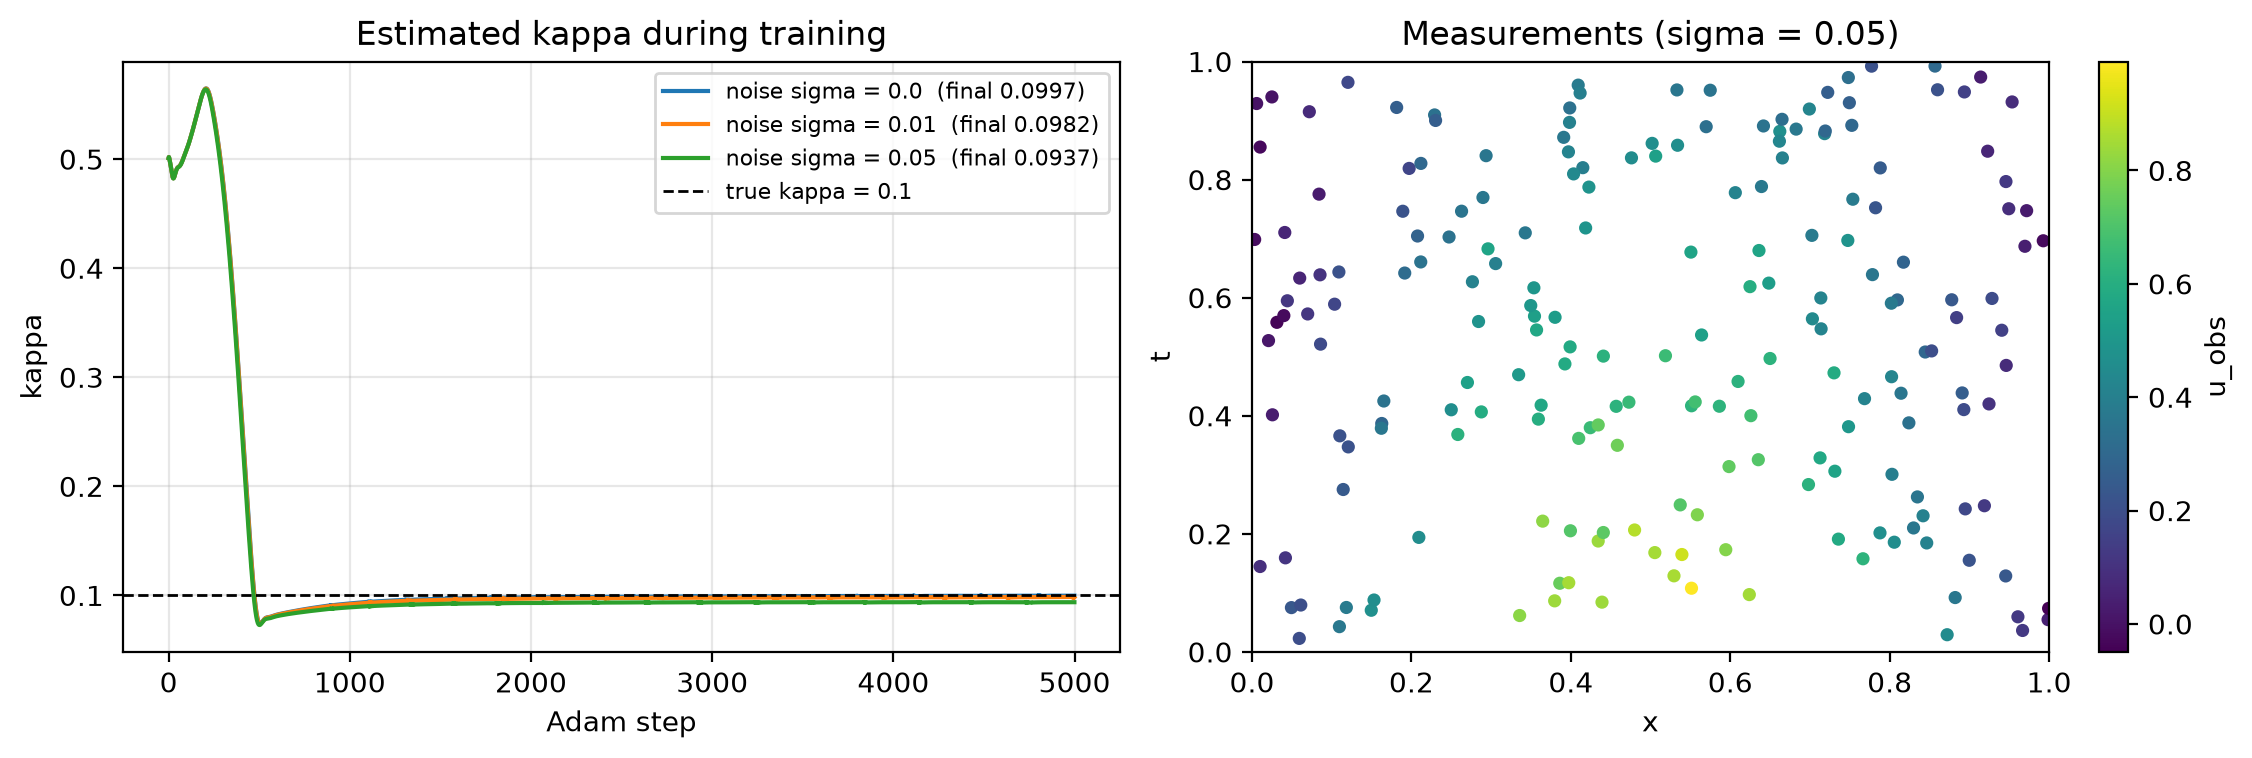
\includegraphics[width=\textwidth]{figures/inverse_kappa.png}

\small 왼쪽: 학습 중 $\kappa$의 변화 (세 곡선이 거의 겹친다). 오른쪽: $\sigma=0.05$일 때의 측정값 $200$개.
\end{center}

\begin{center}
\begin{tabular}{@{}lccc@{}}
\toprule
잡음 $\sigma$ & $0$ & $0.01$ & $0.05$ \\
\midrule
추정한 $\kappa$ (참값 $0.1$) & $0.09975$ & $0.09822$ & $0.09375$ \\
상대오차 $|\kappa_{\text{추정}}-0.1|/0.1$ & $0.25\%$ & $1.8\%$ & $6.3\%$ \\
\bottomrule
\end{tabular}
\end{center}

\begin{itemize}[leftmargin=1.5em]
\item $\kappa$는 처음 $200$ step 동안 $0.56$까지 오른 뒤 $300$--$500$ step 사이에 급격히 내려온다.
초기의 $u_\theta$는 측정값과 맞지 않으므로 그 $u_t$, $u_{xx}$로 정한 $\kappa$도 의미가 없다. $u_\theta$가 측정값에 맞은 뒤에 $\kappa$가 수렴한다.
\item 잡음이 없으면 오차는 $0.25\%$이고, 잡음이 커질수록 오차가 커진다. 이 실험에서는 모두 참값보다 작게 추정되었다.
\item 측정 오차가 추정값에서 증폭되는 것은 역문제의 일반적인 성질 (ill-posedness)이며, 정칙화 등으로 다룬다.
\end{itemize}

% =================================================
\section{2차원 타원형 방정식}\label{sec:elliptic}
% =================================================

\subsection{문제}

단위 원판 $\Omega=\{(x,y):x^2+y^2<1\}$에서 다음 경계값 문제를 푼다.
\begin{equation}\label{eq:elliptic}
\nabla\cdot\big(\sigma(x,y)\,\nabla u\big)=0\quad\text{in }\Omega,\qquad u=\cos\theta\quad\text{on }\partial\Omega.
\end{equation}
$\nabla u=(u_x,u_y)$이고 $\nabla\cdot(\sigma\nabla u)=(\sigma u_x)_x+(\sigma u_y)_y$이다.
$\sigma>0$이면 이 방정식은 \textbf{타원형}이고, Dirichlet 경계조건 하나로 해가 유일하게 정해진다.
$u$는 전위, $\sigma$는 전기전도도로 볼 수 있다: 전류밀도 $-\sigma\nabla u$가 내부에서 생기거나 사라지지 않는다는 식이다.
$\sigma$는 배경값 $1$에 가우스 함수 모양의 덩어리 둘을 더한 것이다.
\[
\sigma(x,y)=1+1.5\,e^{-\frac{(x-0.35)^2+(y-0.2)^2}{2\cdot0.15^2}}-0.5\,e^{-\frac{(x+0.35)^2+(y+0.25)^2}{2\cdot0.18^2}}.
\]
$\sigma$가 상수가 아니므로 정확한 해를 식으로 쓸 수 없어서,
기준 해를 \texttt{fem\_disk.py}의 유한요소법으로 구한다. 삼각형 요소의 노드는 $31731$개이고,
$\sigma=1$일 때 정확한 해와의 오차는 $10^{-5}$ 정도이다.

\subsection{residual: 발산을 자동미분으로}

입력은 \texttt{X} $=(x,y)$, 모양 $(N,2)$이다. $\nabla\cdot(\sigma\nabla u)$는 자동미분 세 번으로 계산한다.
\begin{lstlisting}
def residual(X):
    u = model(X)                                     # (N, 1)
    s = sigma(X[:, 0:1], X[:, 1:2])                  # (N, 1)
    flux = s * grad(u, X)                            # (N, 2) = sigma * (u_x, u_y)
    div = grad(flux[:, 0:1], X)[:, 0:1] + grad(flux[:, 1:2], X)[:, 1:2]   # (sigma u_x)_x + (sigma u_y)_y
    return div
\end{lstlisting}
\texttt{grad(u, X)}는 $(u_x,u_y)$를 한 번에 준다. 플럭스의 첫 열 $\sigma u_x$를 \texttt{X}로 미분한 결과에서 첫 열 ($x$ 미분)을,
둘째 열 $\sigma u_y$를 미분한 결과에서 둘째 열 ($y$ 미분)을 가져와 더한다 (\ref{sec:twoinputs}절과 같은 방법).
$\sigma$의 도함수는 따로 계산하지 않는다. $\sigma$가 \texttt{X}로부터 계산된 텐서이므로 곱의 미분 $(\sigma u_x)_x=\sigma_xu_x+\sigma u_{xx}$를 autograd가 처리한다.

\subsection{점과 loss}

내부 점 $20000$개를 원판에 균일하게 뽑아 두고 ($r=\sqrt{U}$, $\theta=2\pi V$, $U,V\sim\mathcal U(0,1)$), 매 step $1000$개를 미니배치로 쓴다
(\ref{sec:freq}절).
경계점은 $2000$개를 뽑아 두고 매 step $256$개를 쓴다. loss는
\[
\loss=\frac1{1000}\sum_{i}\big(\nabla\cdot(\sigma\nabla u_\theta)\big)^2\Big|_{X_i}+10\cdot\frac1{256}\sum_k\big(u_\theta(X_k)-\cos\theta_k\big)^2
\]
이다. 신경망은 $2\to64\to64\to64\to1$ ($\tanh$), Adam $5000$ step이며, 학습률은 $1667$ step마다 $0.3$배로 줄인다
(\texttt{torch.optim.lr\_scheduler.StepLR}).

\subsection{결과}

GPU (RTX 4070)에서 약 $110$초가 걸렸다. 유한요소 해의 노드 $31731$개에서 잰 상대오차는 $2.9\times10^{-3}$, 최대 절대오차는 $6.3\times10^{-3}$이다.

\begin{center}
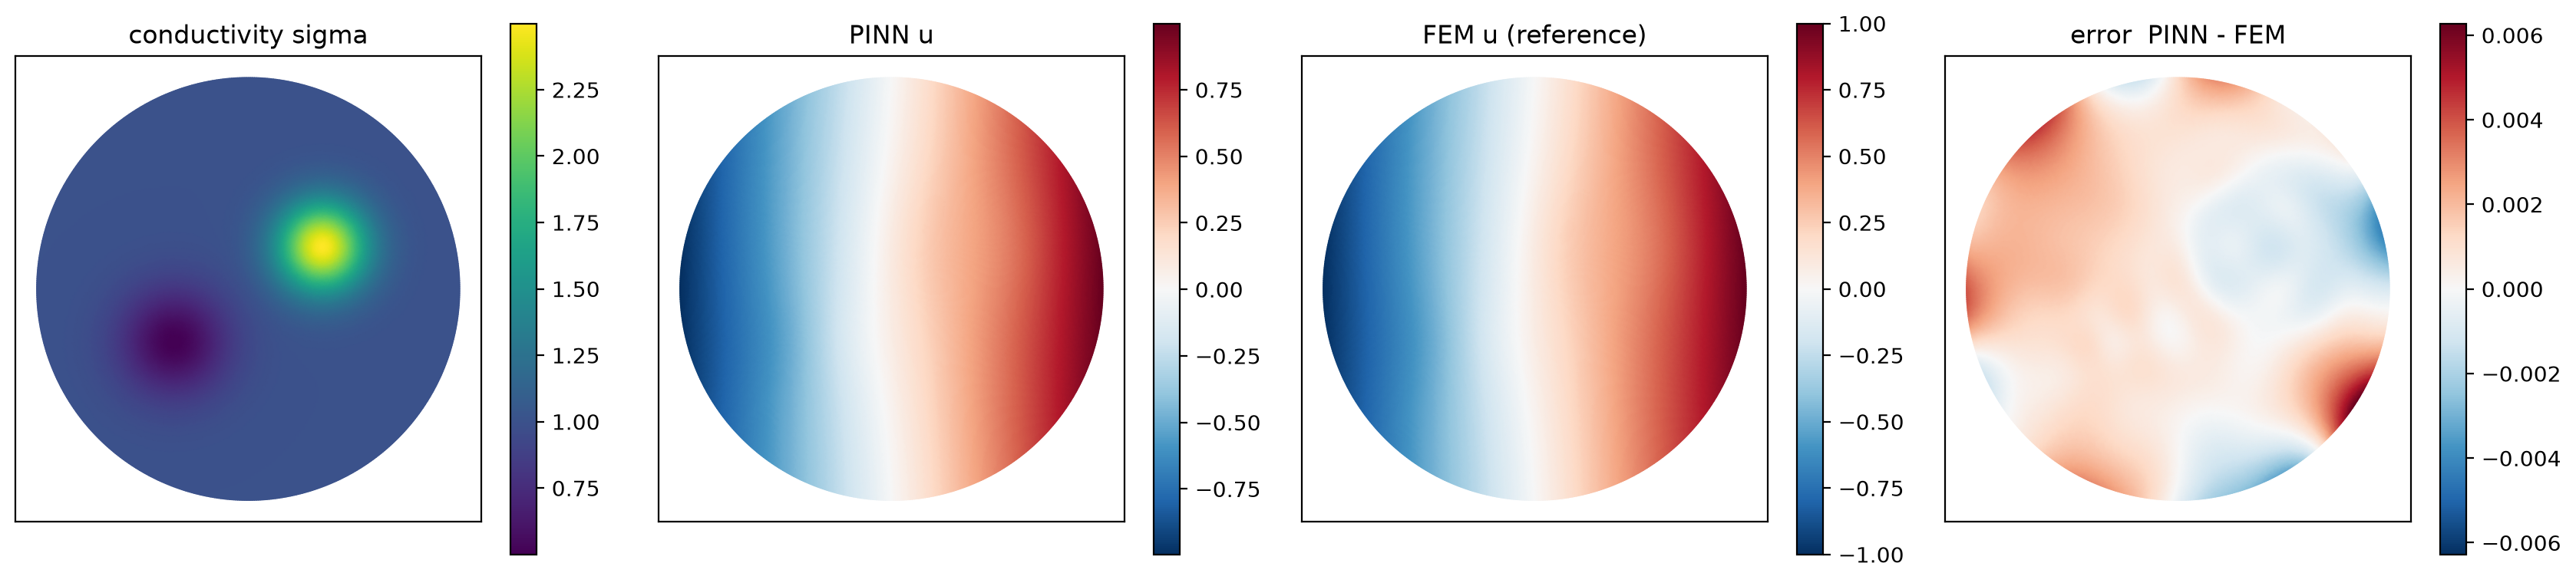
\includegraphics[width=\textwidth]{figures/elliptic_field.png}

\small 왼쪽부터 $\sigma$, PINN의 해, 유한요소 해, 오차.
\end{center}

\begin{center}
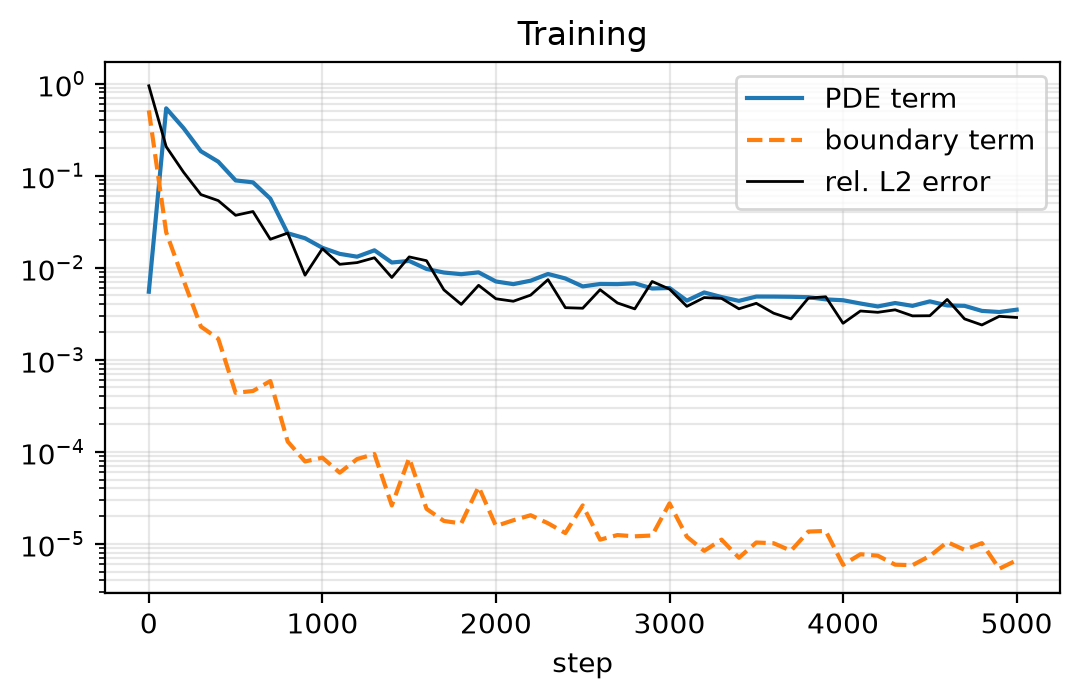
\includegraphics[width=0.55\textwidth]{figures/elliptic_loss.png}

\small loss의 두 항과 상대오차.
\end{center}

\begin{itemize}[leftmargin=1.5em]
\item 해의 등위선이 $\sigma$가 큰 곳 (오른쪽 위)에서는 벌어지고 작은 곳 (왼쪽 아래)에서는 좁아진다. 전도도가 큰 곳에서는 작은 전위차로도 같은 전류가 흐르기 때문이다.
\item 처음 PDE 항은 $5\times10^{-3}$으로 작고 경계 항이 $0.5$로 크다. 초기 신경망은 거의 상수이고, 상수 함수는 방정식 \eqref{eq:elliptic}을 만족한다 (\ref{sec:heat}절과 같은 현상).
\item 오차가 가장 큰 곳은 경계 근처이다.
\end{itemize}

% =================================================
\section{역문제 2: 전기 임피던스 단층촬영 (EIT)}\label{sec:eit}
% =================================================

\subsection{문제}

\ref{sec:elliptic}절의 방정식에서 이번에는 $\sigma$를 모른다. 대신 경계에서 전류와 전압을 측정한다.
경계에 전류 $g_j$를 흘려 넣으면 내부의 전위 $u_j$는
\begin{equation}\label{eq:eit}
\nabla\cdot(\sigma\nabla u_j)=0\quad\text{in }\Omega,\qquad \sigma\,\partial_nu_j=g_j\quad\text{on }\partial\Omega
\end{equation}
를 만족하고, 경계의 전압 $f_j=u_j|_{\partial\Omega}$를 측정할 수 있다 ($\partial_n$은 바깥 법선 방향의 미분).
전류--전압 쌍 $(g_j,f_j)$ 여러 개로부터 내부의 전도도 $\sigma$를 찾는 문제가 \textbf{전기 임피던스 단층촬영} (EIT)이다.
여기서는 전극을 따로 생각하지 않고, 경계 전체에서 전압을 측정한다고 둔다.

\begin{itemize}[leftmargin=1.5em]
\item 전류: $g_j=\cos n\theta,\ \sin n\theta$ ($n=1,\dots,4$), 모두 $J=8$쌍.
\item 전압: 참값 $\sigma$ (\ref{sec:elliptic}절의 것)로 유한요소법을 풀어 만든 $f_j$를 경계의 $4096$개 점에서 준다. PINN은 참값 $\sigma$를 모른다.
\end{itemize}

데이터 한 쌍을 그려 보자 (\texttt{eit\_boundary\_data.py}).
첫 번째 쌍 $j=1$은 전류 $g_1=\cos\theta$를 흘려 넣고 전압 $f_1$을 잰 것이다.
$\sigma\equiv1$이면 $u=r\cos\theta$이므로 전압은 정확히 $\cos\theta$이다.
실제 전압과 $\cos\theta$의 차이는 최대 $0.053$ (약 $5\%$)이고, 내부의 $\sigma$에 대한 정보는 이 작은 차이에만 들어 있다.

\begin{center}
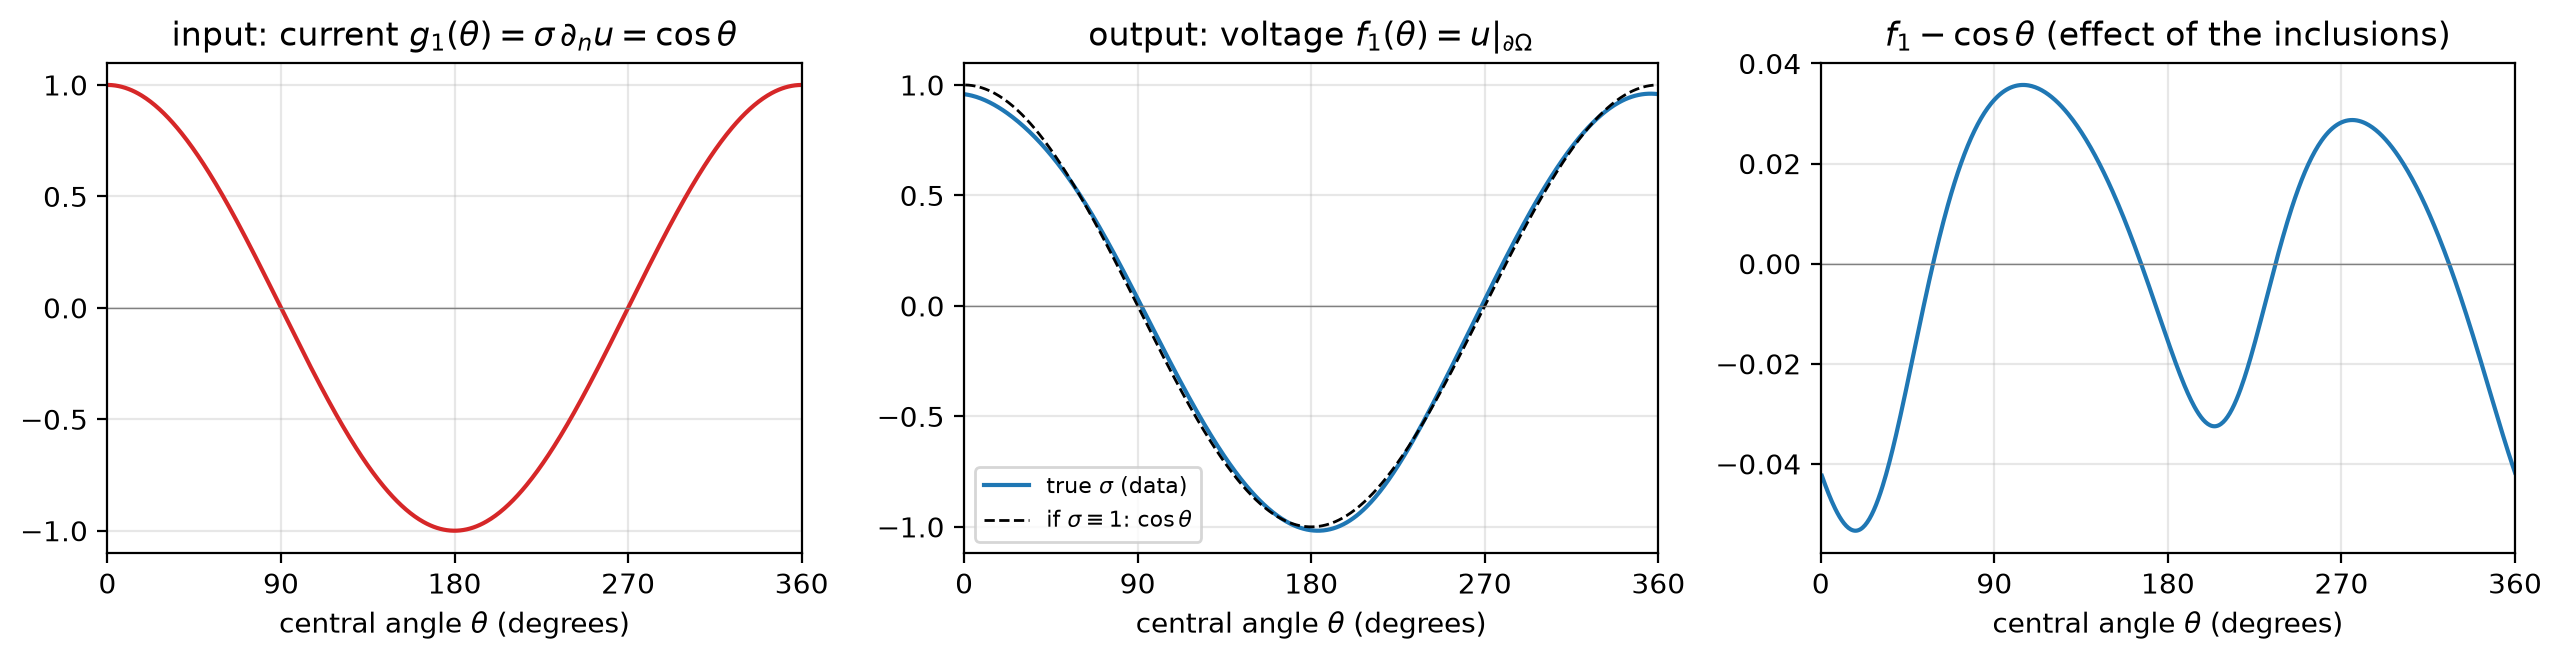
\includegraphics[width=\textwidth]{figures/eit_data_theta.png}

\small 중심각 $\theta$에 대한 첫 번째 쌍. 왼쪽: 입력 전류 $g_1$. 가운데: 측정한 전압 $f_1$ (점선은 $\sigma\equiv1$일 때의 $\cos\theta$). 오른쪽: 둘의 차이.
\end{center}

\begin{center}
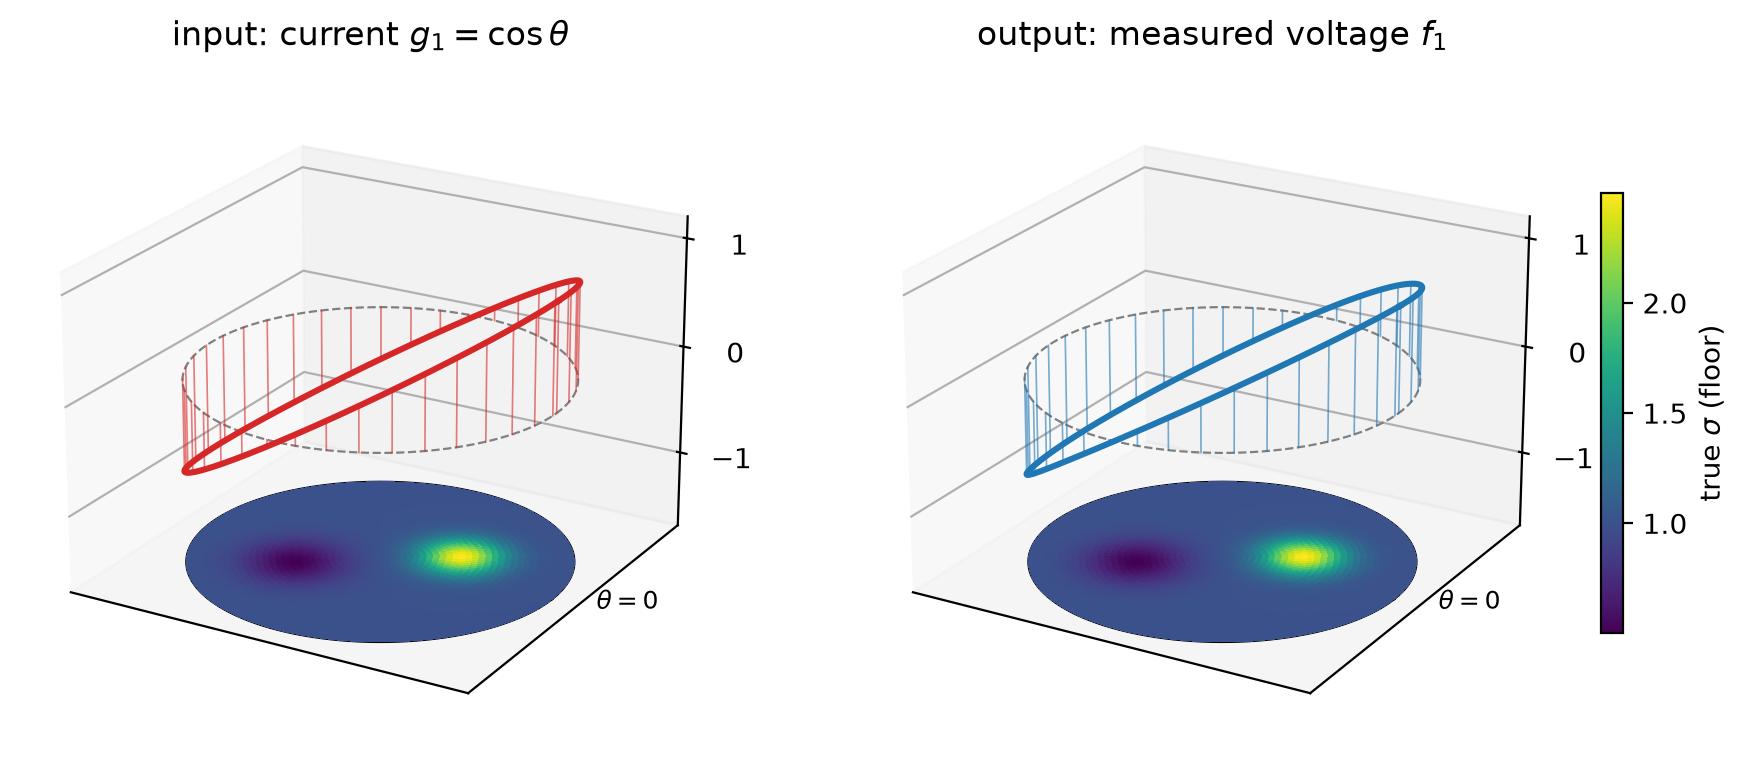
\includegraphics[width=0.8\textwidth]{figures/eit_data_3d.png}

\small 같은 쌍을 원판의 둘레에 그린 것. 바닥은 참값 $\sigma$ (PINN은 모른다), 왼쪽은 전류 $g_1$, 오른쪽은 전압 $f_1$이다.
두 곡선은 거의 같아 보인다. 경계에서 잰 값이 내부의 $\sigma$에 둔감하다는 것이 EIT가 어려운 (ill-posed) 이유이다.
\end{center}

이런 쌍 $J=8$개가 PINN이 보는 데이터의 전부이다.

\subsection{두 개의 신경망}

미지수는 $\sigma$와 $u_1,\dots,u_J$이다. 각각을 신경망으로 둔다.
\[
\sigma(x,y)=s_\phi(x,y),\qquad \big(u_1,\dots,u_J\big)(x,y)=u_\theta(x,y).
\]
$u_\theta$는 입력 $2$개, 출력 $J$개인 신경망 하나이고, $s_\phi$는 입력 $2$개, 출력 $1$개인 신경망이다.
loss는 내부의 residual, 경계의 전압 오차, 경계의 전류 오차의 합이다.
\[
\loss(\theta,\phi)=\frac1J\sum_{j}\frac1{B}\sum_i\big(\nabla\cdot(\sigma\nabla u_j)\big)^2\Big|_{X_i}
+\lambda\,\frac1J\sum_j\frac1{N_b}\sum_k\Big[\big(u_j-f_j\big)^2+\big(\sigma\,\partial_nu_j-g_j\big)^2\Big]\Big|_{X_k}.
\]
\begin{lstlisting}
def loss_terms():
    X = X_f[torch.randint(0, N_f, (batch,), device=device)].clone().requires_grad_(True)
    U, S = u_net(X), s_net(X)
    loss_pde = 0.0
    for j in range(J):
        flux = S * grad(U[:, j:j+1], X)
        div = grad(flux[:, 0:1], X)[:, 0:1] + grad(flux[:, 1:2], X)[:, 1:2]
        loss_pde = loss_pde + torch.mean(div**2) / J
    Xb = X_b.clone().requires_grad_(True)
    Ub, Sb = u_net(Xb), s_net(Xb)
    dudn = torch.cat([(grad(Ub[:, j:j+1], Xb) * Xb).sum(dim=1, keepdim=True)
                      for j in range(J)], dim=1)
    loss_D = torch.mean((Ub - f_b)**2)            # voltage data
    loss_N = torch.mean((Sb * dudn - g_b)**2)     # current data
    return loss_pde, loss_D, loss_N
\end{lstlisting}
residual은 \ref{sec:elliptic}절과 같은 계산을 $J$번 한다.
원판의 경계에서 바깥 법선은 위치 벡터 $(x,y)$ 자체이므로, $\partial_nu=\nabla u\cdot(x,y)$는 \texttt{(grad(...) * Xb).sum(1)}이다.
역전파는 두 신경망의 매개변수 $\theta$, $\phi$ 모두에 gradient를 준다.

\subsection{결과}

$\sigma$의 정확도는 식 \eqref{eq:relerr}에서 분모만 바꾼
\[
\frac{\|s_\phi-\sigma\|_2}{\|\sigma-1\|_2}
\]
로 잰다. 시험점은 $[-1,1]^2$의 $101\times101$ 격자 중 원판 안의 점이다.
분모가 배경값 $1$과의 차이이므로, 경계 데이터를 쓰지 않고 $\sigma\equiv1$로 답하면 이 값은 $1$이다.

전류--전압 쌍은 $J=8$개, 경계점은 $N_b=4096$개, 내부의 collocation point는 $N_f=20000$개이고, 매 step $2000$개를 미니배치로 뽑는다.
가중치는 $\lambda=100$이다. $u_\theta$는 은닉층 $4$개, $s_\phi$는 은닉층 $3$개이고 폭은 모두 $64$, 활성화 함수는 $\tanh$이다.
Adam으로 $150000$ step을 학습하였다. 학습률은 $10^{-3}$에서 시작해 $50000$ step마다 $0.3$배로 줄인다.
GPU (RTX 4070)에서 약 $3.8$시간이 걸렸다.

상대오차는 $0.573$이고, 복원한 $\sigma$의 범위는 $[0.73,\,1.48]$이다 (참값 $[0.50,\,2.50]$).

\begin{center}
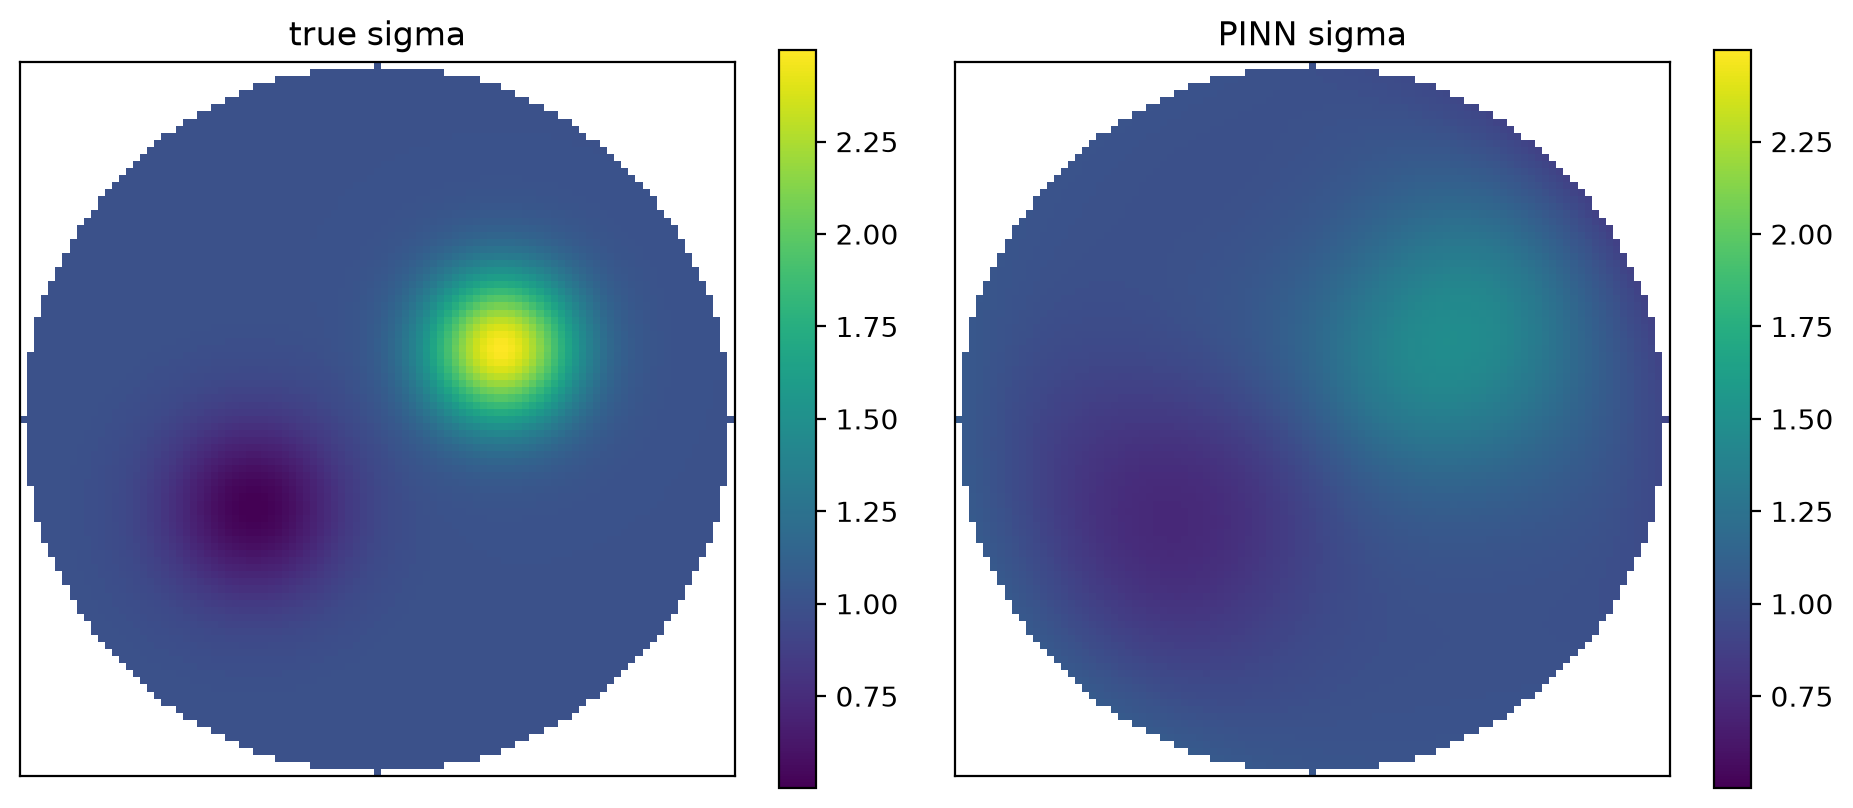
\includegraphics[width=0.85\textwidth]{figures/eit_sigma.png}

\small 왼쪽: 참값 $\sigma$. 오른쪽: PINN이 경계의 전류--전압 쌍 $8$개에서 복원한 $\sigma=s_\phi$. 색의 범위는 같다.
\end{center}

\begin{center}
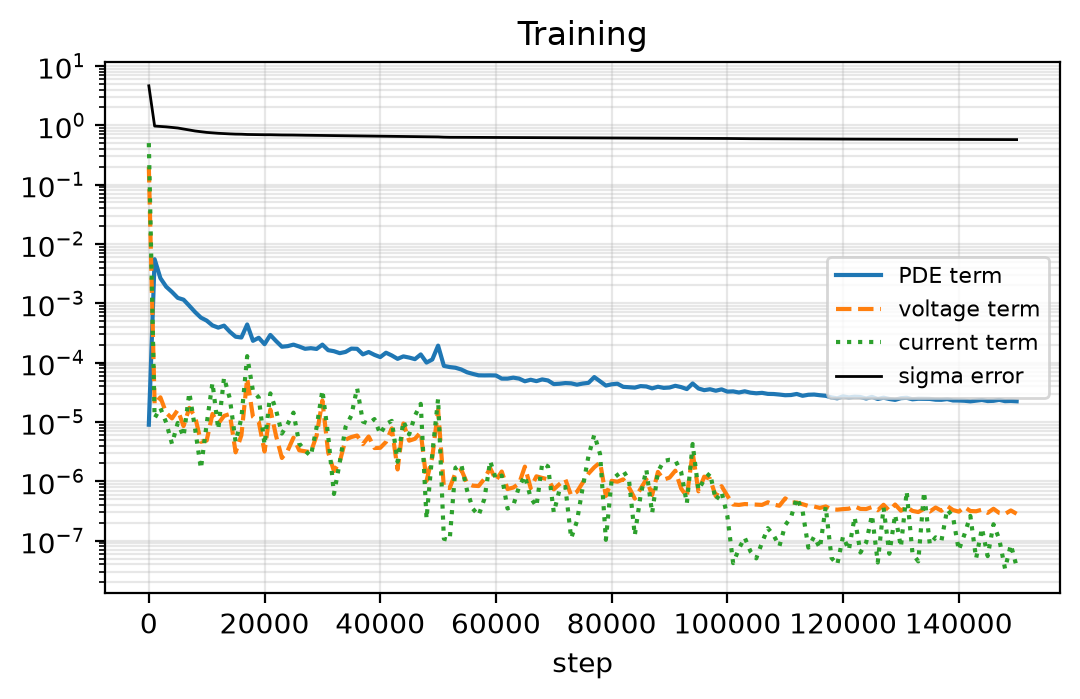
\includegraphics[width=0.62\textwidth]{figures/eit_loss.png}

\small loss의 세 항과 $\sigma$의 상대오차.
\end{center}

\begin{itemize}[leftmargin=1.5em]
\item $\sigma>1$인 덩어리와 $\sigma<1$인 덩어리의 위치를 찾았다. 신경망에게 $\sigma$의 값을 직접 알려 준 적은 없다.
\item 복원한 덩어리는 참값보다 넓게 퍼져 있고 진폭이 작다.
\item 마지막 step에서 PDE 항은 $2.2\times10^{-5}$, 전압 항은 $2.8\times10^{-7}$, 전류 항은 $3.7\times10^{-8}$이다. loss가 이렇게 작아도 $\sigma$의 오차는 $0.573$이다. 경계 측정값을 거의 맞추어도 내부의 $\sigma$까지 정확한 것은 아니다. EIT는 ill-posed 문제이다.
\end{itemize}

\begin{remarkbox}[학습에 영향을 주는 것들]
역문제의 결과는 다음 값들에 크게 좌우되므로 여러 값을 시험해 보아야 한다.
\begin{itemize}[leftmargin=1.5em]
\item 전류--전압 쌍의 수, 경계점과 내부 collocation point의 수, 미니배치 크기.
\item loss 항들의 가중치 $\lambda$.
\item step 수, 학습률 schedule, 두 신경망의 크기.
\item 경계 데이터의 잡음.
\end{itemize}
\end{remarkbox}

% =================================================
\section{PINN의 한계와 요령}\label{sec:limits}
% =================================================

\subsection{높은 주파수와 collocation point의 수}\label{sec:freq}

\texttt{pinn\_frequency.py}의 셀 1은 \ref{sec:poisson}절과 같은 신경망, 같은 점 $64$개, 같은 Adam $5000$ step으로 다음 문제를 푼다.
\[
-u''=(k\pi)^2\sin(k\pi x),\qquad u(0)=u(1)=0,\qquad k=1,2,4,8.
\]
정확한 해는 $\sin(k\pi x)$이다. 비교를 위해 residual을 $(k\pi)^2$로 나누어 loss의 크기를 맞추었다.

\begin{center}
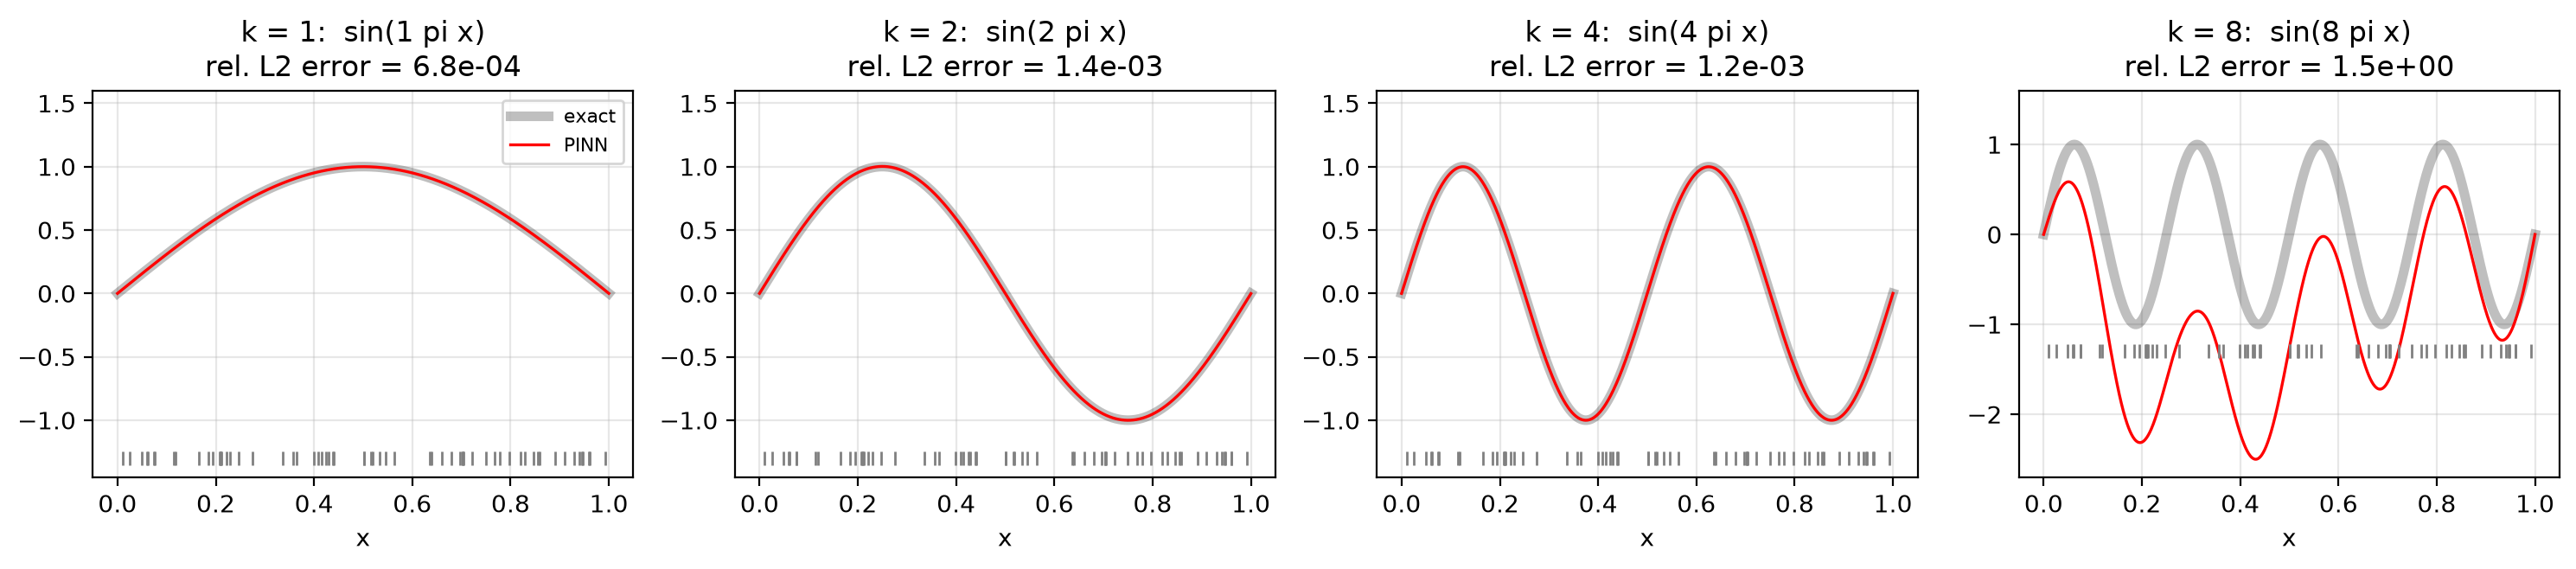
\includegraphics[width=\textwidth]{figures/frequency.png}

\small 같은 조건으로 학습하면 $k=8$에서 실패한다 (마지막 그림은 세로축 범위가 다르다).
\end{center}

\begin{center}
\begin{tabular}{@{}lcccc@{}}
\toprule
$k$ & $1$ & $2$ & $4$ & $8$ \\
\midrule
마지막 loss (나눈 뒤) & $4.1\times10^{-6}$ & $3.2\times10^{-6}$ & $8.7\times10^{-6}$ & $4.5\times10^{-4}$ \\
상대오차 & $6.8\times10^{-4}$ & $1.5\times10^{-3}$ & $1.2\times10^{-3}$ & $1.5$ \\
\bottomrule
\end{tabular}
\end{center}

\begin{center}
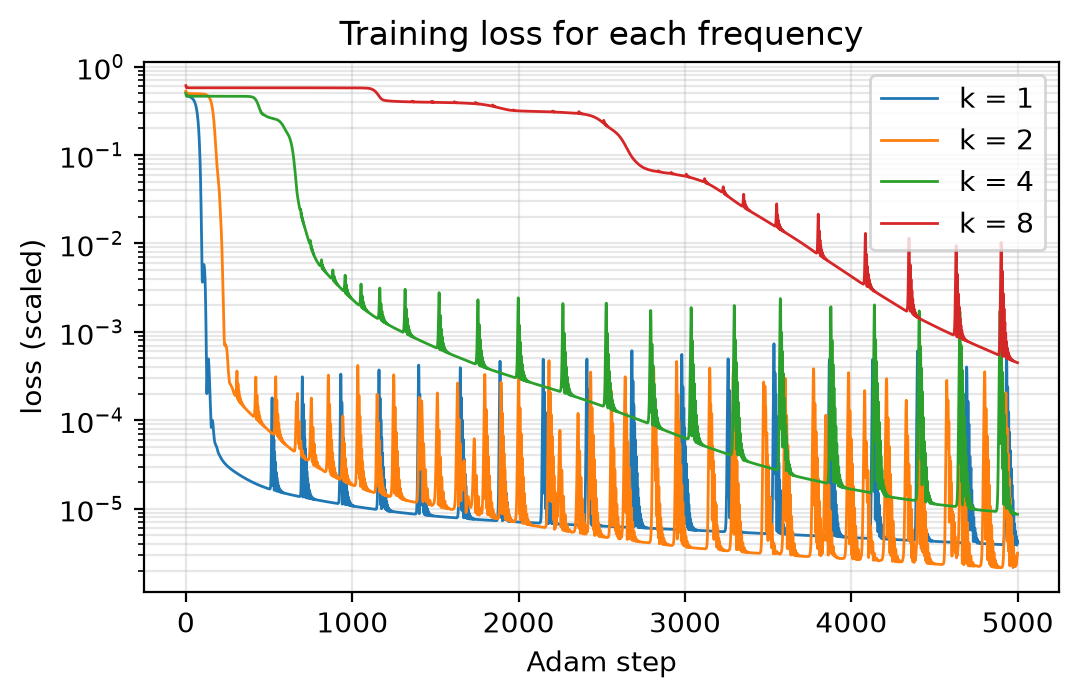
\includegraphics[width=0.55\textwidth]{figures/frequency_loss.png}

\small 진동수별 학습 곡선.
\end{center}

원인을 보려고 셀 3에서는 $k=8$을 세 조건으로, 조건마다 seed $3$개로 푼다.
residual은 학습에 쓴 점 (훈련)과 $[0,1]$의 $1001$개 격자점 (테스트)에서 따로 잰다. 지도학습의 훈련 오차와 테스트 오차에 해당한다.
세 번째 조건은 collocation point $10000$개를 만들어 두고 매 step $256$개를 무작위로 뽑아 쓰는 \textbf{미니배치} 학습이다.

\begin{center}
\small
\begin{tabular}{@{}llccc@{}}
\toprule
조건 & seed & 훈련 residual$^2$ & 테스트 residual$^2$ & 상대오차 \\
\midrule
점 $64$개, $5000$ step & $0$ & $4.5\times10^{-4}$ & $3.8\times10^{-3}$ & $1.5$ \\
 & $1$ & $1.4\times10^{-1}$ & $2.5\times10^{-1}$ & $10$ \\
 & $2$ & $1.1\times10^{-2}$ & $3.3\times10^{-2}$ & $7.9$ \\
\midrule
점 $64$개, $20000$ step & $0$ & $8.3\times10^{-6}$ & $2.7\times10^{-4}$ & $0.39$ \\
 & $1$ & $1.6\times10^{-3}$ & $1.0\times10^{-1}$ & $4.5$ \\
 & $2$ & $2.0\times10^{-5}$ & $6.5\times10^{-3}$ & $1.7$ \\
\midrule
점 $10000$개 (미니배치 $256$), & $0$ & $5.8\times10^{-5}$ & $6.1\times10^{-5}$ & $0.0076$ \\
$20000$ step & $1$ & $1.4\times10^{-5}$ & $1.4\times10^{-5}$ & $0.015$ \\
 & $2$ & $2.6\times10^{-6}$ & $2.7\times10^{-6}$ & $0.027$ \\
\bottomrule
\end{tabular}
\end{center}

\begin{center}
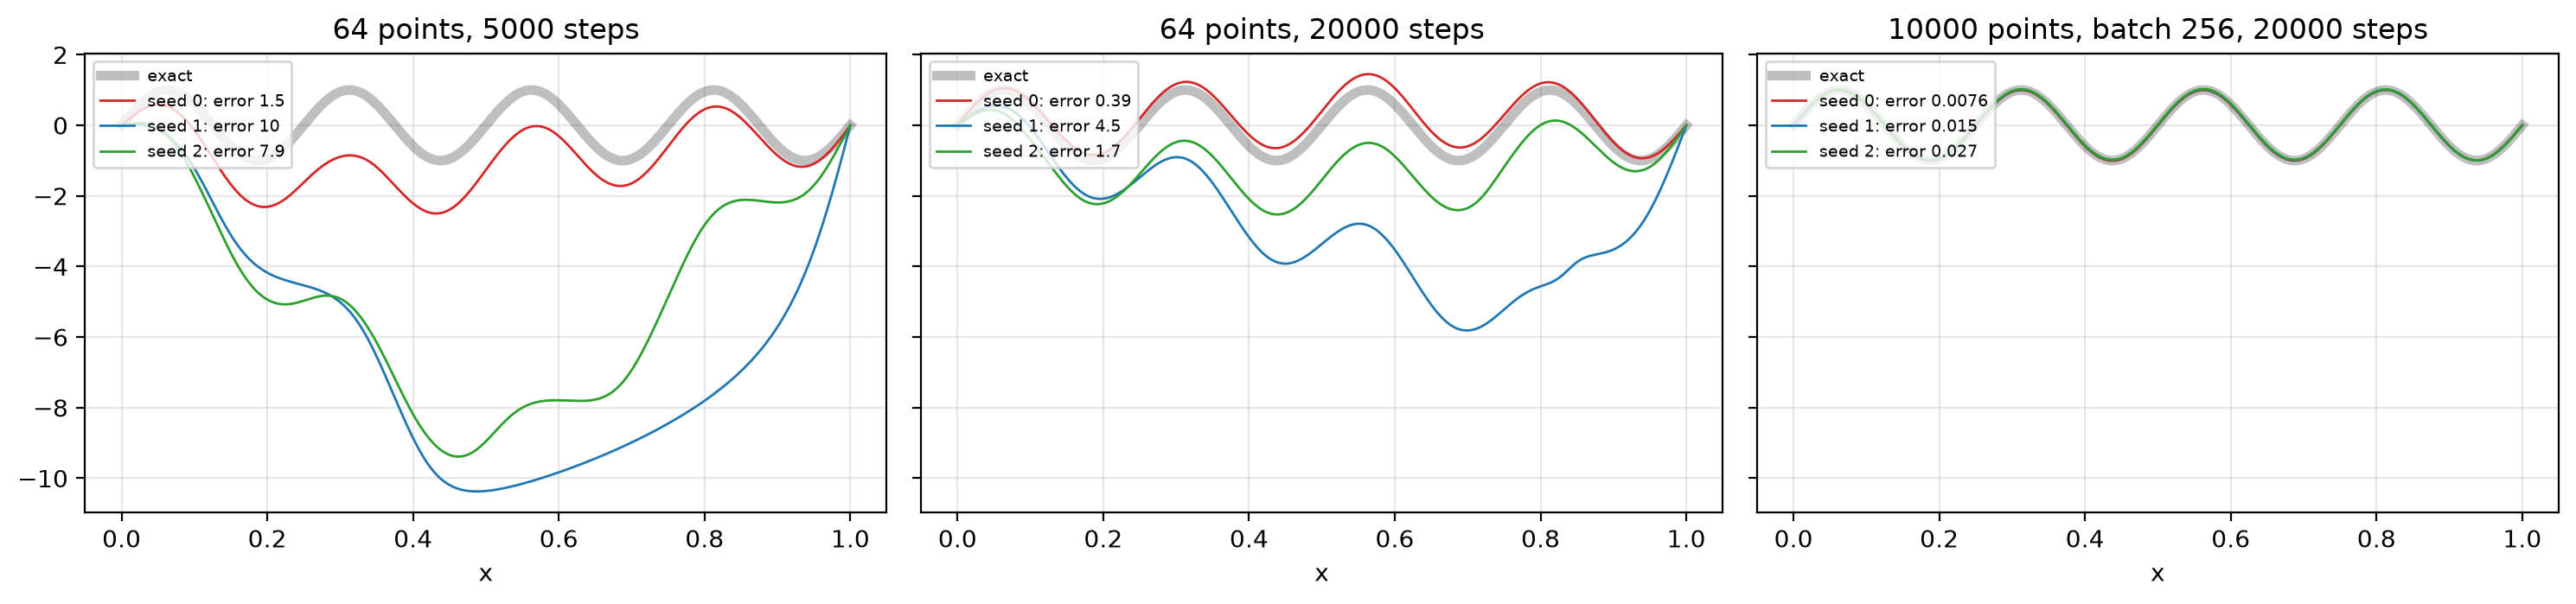
\includegraphics[width=\textwidth]{figures/frequency_k8.png}

\small $k=8$의 세 조건. 각 그림에 seed $3$개의 결과를 겹쳐 그렸다.
\end{center}

\begin{itemize}[leftmargin=1.5em]
\item 점이 $64$개이면 훈련 residual이 테스트 residual보다 작고, 학습을 오래 할수록 그 차이가 커진다 ($5000$ step에서 $2$--$8$배, $20000$ step에서 $30$--$300$배).
신경망이 $64$개 점에서만 방정식을 만족하고 점 사이에서는 만족하지 않는, collocation point에 대한 \textbf{과적합}이다.
\item 점이 $10000$개이면 훈련과 테스트 residual이 같고, 상대오차는 $0.008$--$0.03$이다.
\item 해가 빠르게 진동할수록 방정식을 만족해야 할 정보가 많으므로 점이 더 많이 필요하다.
또 경사하강법으로 학습하는 신경망은 낮은 주파수 성분을 먼저 학습하는 경향 (\textbf{spectral bias})이 있어서, 높은 주파수의 해에는 step도 더 많이 필요하다.
\end{itemize}
collocation point는 계산으로 얼마든지 만들 수 있으므로, 지도학습과 달리 훈련 데이터의 양에 제한이 없다.
실제 PINN에서는 점을 충분히 많이 만들어 두고 미니배치로 오래 학습한다.
그 밖에 입력 $x$ 대신 $\big(\sin(2\pi\omega_jx),\cos(2\pi\omega_jx)\big)_j$를 넣는 방법 (Fourier feature),
영역을 나누어 각각 작은 신경망을 쓰는 방법 등이 있다.

\subsection{loss 항의 균형}

PINN의 loss는 성격이 다른 항의 가중합이다. Poisson 문제의 처음 loss에서 PDE 항은 $46$, 경계 항은 $0.03$이었다.
크기가 크게 다르면 gradient가 큰 항만 줄어든다. 그래서 $\lambda$를 조절하거나, 학습 중 각 항의 gradient 크기에 따라 가중치를 자동으로 바꾸는 방법을 쓴다.
적절한 가중치는 문제마다 다르다.

\subsection{고전적인 수치해법과 비교하면}

같은 Poisson 문제를 \textbf{유한차분법}으로 풀면 (\texttt{pinn\_poisson\_1d.py}의 182--193줄),
$u''(x_i)\approx(u_{i-1}-2u_i+u_{i+1})/\Delta x^2$에 의해 연립일차방정식 하나가 된다.

\begin{remarkbox}[수치해법으로서의 PINN]
두 방법 모두 해를 유한 개의 미지수로 표현하고, 방정식을 유한 개의 점에서 만족시킨다.
\begin{itemize}[leftmargin=1.5em]
\item 유한차분법: 미지수는 격자점의 값 $u_1,\dots,u_{n-1}$이고 도함수를 차분으로 근사한다. 선형 미분방정식은 연립일차방정식 $A\vect u=\vect b$가 된다.
\item PINN: 미지수는 $\theta$이고 근사해의 공간은 $\{u_\theta\}$이다. 도함수는 자동미분으로 (반올림 오차 안에서) 정확히 계산하고,
collocation point에서의 residual을 최소제곱으로 줄인다. 방정식이 선형이어도 $u_\theta$는 $\theta$에 대해 비선형이므로 비볼록 최적화 문제가 된다.
\end{itemize}
\end{remarkbox}

\begin{center}
\begin{tabular}{@{}lcc@{}}
\toprule
방법 & 상대오차 & 시간 \\
\midrule
유한차분법 (구간 $100$개, CPU) & $8.2\times10^{-5}$ & 약 $1$--$10$ ms \\
PINN (Adam $5000$ step, GPU) & $6.1\times10^{-5}$ & 약 $40$ s \\
PINN (Adam $5000$ step + L-BFGS, GPU) & $1.5\times10^{-5}$ & 약 $40$ s \\
\bottomrule
\end{tabular}
\end{center}

이런 \textbf{순문제}에서 PINN은 유한차분법, 유한요소법보다 수천 배 느리고 오차에 대한 이론적 보장도 약하다. PINN이 유리한 경우는 다음과 같다.
\begin{itemize}[leftmargin=1.5em]
\item \textbf{역문제}와 데이터 동화: 측정값과 방정식을 하나의 loss로 결합한다 (\ref{sec:inverse}절). 코드는 순문제와 거의 같다.
\item \textbf{격자가 필요 없다}: 점만 뽑으면 되므로 복잡한 영역이나 고차원 문제에 적용하기 쉽다.
\item 방정식의 일부만 알거나 데이터가 흩어져 있는 경우.
\end{itemize}

\subsection{더 나아가: 연산자를 배우기}

PINN은 주어진 $f$, $\kappa$ 하나에 대한 해를 구하며, 이들이 바뀌면 다시 학습해야 한다.
이와 달리 해 연산자 $f\mapsto u$를 신경망으로 근사하는 방법이 있다. DeepONet (2021)과 Fourier Neural Operator (FNO, 2021)가 대표적이며,
학습 후에는 새로운 $f$에 대한 해를 forward 한 번으로 얻는다.

% =================================================
\section{정리}\label{sec:summary}
% =================================================

\begin{keybox}[PINN: 정리]
\begin{itemize}[leftmargin=1.5em]
\item PINN은 신경망 $u_\theta$의 residual (방정식을 어기는 정도)과 초기/경계조건 오차를 loss로 하여 미분방정식을 푼다.
\item 입력에 대한 미분 $u_x$, $u_{xx}$는 \texttt{autograd.grad(..., grad\_outputs=ones\_like(u), create\_graph=True)}로 구한다.
이 계산은 원래 그래프에 매달린 미분 그래프를 만들며, residual이 둘을 하나의 그래프로 잇는다.
\item \texttt{loss.backward()}는 합쳐진 그래프를 거꾸로 지나며, 한 가중치에서 출발한 여러 경로의 기여를 \textbf{더한다}.
optimizer는 이 사실을 모르고 \texttt{.grad}만 쓴다.
\item 입력이 여러 개이면 \texttt{grad}의 결과에서 필요한 열을 잘라 쓴다. 모양 $(N,1)$을 유지하자.
\item 역문제에서는 미지의 계수를 \texttt{nn.Parameter}로 두고 측정값 항과 방정식 항을 함께 최소화한다.
미지의 계수가 함수이면 ($\sigma(x,y)$, EIT) 그것도 신경망으로 둔다.
\item 해가 빠르게 진동할수록 collocation point가 많이 필요하다. 점이 적으면 점에서만 방정식을 만족하는 과적합이 일어난다. 점을 충분히 만들어 두고 미니배치로 오래 학습한다.
\item 한계: loss 항의 균형, 계산 비용. 순문제에서는 고전적인 수치해법이 훨씬 빠르다.
PINN의 강점은 역문제, 데이터와 방정식의 결합, 격자가 필요 없다는 점이다.
\end{itemize}
\end{keybox}

% =================================================
\section{연습문제}
% =================================================

\begin{enumerate}[label=\arabic*.]

\item \ref{sec:tiny}절의 신경망에서 $x=0$일 때 $a$, $h$, $u$, $u_x$, $u_{xx}$를 손으로 계산하라 ($\tanh(-0.2)\approx-0.19738$).
\texttt{autograd\_tiny.py}의 \texttt{x}를 바꾸어 확인하라.

\item \ref{sec:backward}절의 그래프에서 $\partial\loss/\partial b_2$의 경로가 하나뿐인 이유를 설명하라.
$\loss$가 $u''+u=0$ 대신 $u''=0$의 residual $r=u_{xx}$로 만들어졌다면 $\partial\loss/\partial b_2$는 얼마인가? 그 이유는?
이것이 \ref{sec:poisson}절에서 경계 항이 필요한 이유와 어떻게 관련되는지 설명하라.

\item \texttt{pinn\_poisson\_1d.py}의 \texttt{derivative} 함수에서 \texttt{create\_graph=True}를 지우고 실행해 보라.
어떤 오류가 어느 줄에서 나는가? 첫 번째 \texttt{derivative} 호출에서만 지우면 어떻게 되는가?

\item \texttt{pinn\_poisson\_1d.py}의 \texttt{nn.Tanh()}를 \texttt{nn.ReLU()}로 바꾸어 학습시켜라.
오류가 나는가? loss와 상대오차는 어떻게 되는가? \ref{sec:smooth}절을 이용해 설명하라.

\item \texttt{pinn\_poisson\_1d.py}에서 경계 항의 가중치 \texttt{lam\_b}를 $0$, $0.01$, $1$, $100$으로 바꾸어 상대오차를 비교하라.
$\lambda=0$일 때 얻은 해는 어떤 모양인가? 그 해도 방정식 $-u''=f$는 만족하는가?

\item 같은 코드에서 collocation point를 처음에 한 번 뽑지 않고 \textbf{매 step 새로 뽑도록} 고쳐라
(힌트: 학습 루프 안에서 \texttt{x\_f}를 다시 만든다. \texttt{requires\_grad\_}도 잊지 말자).
residual 그림 (d)가 어떻게 바뀌는지 비교하라.

\item \texttt{pinn\_heat\_1d.py}에서 $\kappa=0.5$로 바꾸어 풀어라 (정확한 해의 식도 같이 바뀐다).
$t=1$에서의 해의 크기는 정확한 해로 얼마여야 하는가? PINN의 결과와 비교하라.

\item \texttt{pinn\_inverse\_heat.py}에서 측정값의 수 \texttt{N\_d}를 $200$에서 $20$, $50$으로 줄여 $\kappa$의 추정값을 비교하라.
측정값을 모두 $t<0.1$에서만 얻는다면 $\kappa$를 잘 찾을 수 있을까? 예상한 뒤 실험으로 확인하라.

\item (생각해 보기) 열 방정식의 측정값이 모두 $x=0.5$ 근처 한 점에서만 얻어졌다면 $\kappa$를 정할 수 있을까?
측정값이 정확한 해 $e^{-\kappa\pi^2t}\sin(\pi x)$에서 나왔다는 것을 이용해 생각해 보라.

\end{enumerate}

\end{document}
